\chapter{Meteorología Agrícola}

\section{Introducción}
\subsection{Conceptos}
¿Quién estudia el tiempo Atmosférico? la respuesta es la Meteorología. Pero ¿Qué estudia la Meteorología? estudia el tiempo atmosférico así como estudia los fenómenos físicos en toda la atmósfera, las causas que los originan y los diferentes métodos de medirlos y observarlos
\begin{definition}[Tiempo Atmosférico]
Es el estado de la atmósfera reinante durante un lapso por lo general breve o en un instante y en un lugar determinado
\end{definition}

\begin{definition}[Climatología]
    Es la parte de la meteorología que basándose en el análisis estadístico de los fenómenos atmosféricos caracteriza el comportamiento de éstos en un lugar determinado, definiendo así su clima.

    Es la rama de la geografía física que tiene por objeto el estudio del clima
\end{definition}

\begin{definition}[Geografía física]
    Es la ciencia que estudia los paisajes naturales de la superficie terrestre, su descripción, causas que originan los diversos tipos y su repetición en las diferentes regiones de la tierra
\end{definition}

\begin{definition}[Clima]
    Son las condiciones medias de los fenómenos atmosféricos que caracterizan una región.
\end{definition}

\begin{example}
El tiempo atmosférico probable para mañana en un lugar dado será caluroso y húmedo, con vientos fuertes y presión baja, a pesar de que el clima del lugar sea templado y seco.
\end{example}

Diferencias entre la meteorología y la climatología:

\begin{itemize}
    \item \textbf{Campo de estudio}. La meteorología estudia toda la atmósfera desde la superficie terrestre hasta su límite superior, en cambio la climatología estudia la capa atmosférica en contacto con la superficie terrestre
    \item \textbf{Tiempo de estudio}. La meteorología se basa en observaciones aisladas no así la climatología que requiere de observaciones hechas con regularidad y por lo menos durante 30 años
    \item \textbf{Aplicación.} La meteorología ayuda a la toma de decisiones operativas y la climatología para la planeación. 
\end{itemize}

\subsubsection{Elementos del tiempo o del clima}

El estado del tiempo durante un lapso definido se caracteriza en cualquier lugar por la presencia e intensidad de una serie de fenómenos meteorológicos por lo general perceptibles cada uno de ellos por nuestros sentidos.

Estos fenómenos en forma conjunta constituyen y caracterizan el estado del tiempo y aisladamente representan los elementos del tiempo o el clima.
Son los fenómenos físicos que se presentan en la atmósfera terrestre y éstos son:
\begin{enumerate}
    \item Radiación solar
    \item Temperatura Presión atmosférica
    \item Viento
    \item Evaporación
    \item Humedad Atmosférica
    \item Nubosidad
    \item Precipitación
\end{enumerate}

\subsubsection{Factores del tiempo o del clima}
Son las causas que hacen variar a los elementos del tiempo o el clima de un lugar a otro y de una estación a otra. Son las condiciones geográficas fijas como:
\begin{enumerate}
    \item Latitud
    \item Altitud
    \item Relieve
    \item Corrientes marinas
    \item Distribución de tierras y aguas
    \item Circulación general de la atmósfera
    \item Trayectoria de las tormentas tropicales
\end{enumerate}

\subsubsection{Clima y sistema climático}

El sistema climático se considera formado por cinco elementos. La atmósfera (la capa gaseosa que envuelve la Tierra), la hidrosfera (el agua dulce y salada en estado líquido), la criosfera (el agua en estado sólido), la litosfera (el suelo) y la biosfera (el conjunto de seres vivos que habitan la Tierra). El clima es consecuencia del equilibrio que se produce en la interacción entre esos cinco componentes.

El sistema climático es el fruto de la interacción de una serie de subsistemas, los que poseen diversas propiedades físicas que se expresan a través de fuertes interconexiones, por medio de las cuales se transfiere energía, momento y materia.

Los subsistemas que dan forma a la globalidad del sistema climático son la atmósfera, la litosfera, la hidrosfera, la criosfera, y la biosfera; todos estos subsistemas se hallan controlados por la influencia de la radiación solar, la única fuente de energía de carácter significativo.

\subsection{Importancia de la meteorología Agrícola}

El 85\% de las tierras de cultivo es de temporal a escala mundial, por lo que es evidente, que gran parte de la agricultura mundial depende de la precipitación y la producción variará según la cantidad de ésta.\footnote{La temperatura, es un elemento climático fundamental que delimita las áreas de producción agrícola.}

La población mundial es de 7927 millones de personas. Un estudio de la Universidad de California, que en general se considera como confiable, estima que las tierras del planeta y sus recursos hidráulicos pueden alimentar como máximo, 8000 millones de personas, bajo las restricciones del estudio.\footnote{Thompson (1975) estima que entre el 60 y 80\% de la variación de la producción de los cultivos, es el resultado de los cambios climáticos.}
Aunque pueden modificarse hasta cierto punto los efectos del tiempo y el clima en los cultivos, la mayor parte del suministro mundial de alimentos, depende aún del tiempo atmosférico y el clima.

Otro aspecto importante es la proporción de crecimiento de la producción de alimentos y de la población, la primera es aritmética (lineal, Z) y la segunda es geométrica (exponencial, Y), lo cual trae como consecuencia que exista tanto en el ámbito mundial como nacional, una notoria escasez de alimentos básicos y conforme transcurre el tiempo se va haciendo más crítica.
\subsubsection{Objetivos}
Mejorar la producción agrícola al relacionar la fenología de los cultivos con la previsión precisa de las condiciones atmosféricas y el conocimiento adecuado de los riesgos del clima, con la finalidad de controlar, prevenir o combatir los elementos atmosféricos. 

Se define en espacio tiempo que elemento o elementos limitan la produccióm agrícola. Obtener la probabilidad de ocurrencia de los elementos del clima con la finalidad de aprovechar los benefpicios y atenuar los prejudiciales.

Determinar si los cultivos perennes o anuales estpan ubicados en las mejores áreas y para estos últimos definir además si están situados en la mejor época.
Dentro de la agrofísica, se divida en la meteorología, con una sola rama que es la micrometeorología y finalmente en la micrometeorología
las ciencias que se relacionan con la meteorología agrícola, son:
\begin{itemize}
    \item Instrumental meteorológico
    \item meteorología
    \item Estadística
    \item Climatología
    \item Ciencia de los cultivos
    \item Edafología
    \item Hidrología
    \item Ciencia Animal
\end{itemize}

\Schema{-1.4ex}{10ex}{\schemabox{Variables en la\\
meteorología agrícola}}{\Schema{-1ex}{4ex}
	{\schemabox{Metereológicas}}
	{{\schemabox{Básicas}}\medskip\schemabox{Generadas}
	}
	\Schema{-1ex}{4ex}
	{\schemabox{Agrometereológicas}}{\schemabox{Fenológicas específicas \\
	\schemabox{Fenológicas no específicas}}}}

\textbf{Meteorológicas:} Representan la concepción física del fenómeno y están definidas por la época de establecimiento del cultivo.

\textbf{Básicas:} son aquellas variables meteorológicas que se les da tratamiento estadístico elemental. 

\textbf{Generadas} Se derivan de las variables meteorológicas básicas o porque a éstas se les da estadístico probabilístico.

\textbf{Agrometeorológicas:}

Éstas representan una relación entre la variable física y el individuo

\textbf{Fenológicas específicas:} Hacen referencia a la reacción que producen en desarrollo) en una etapa delos cultivos (muerte, crecimiento

\textbf{Fenológicas no específicas:} Hacen referencia a la reacción que producen en los cultivos (muerte, crecimiento desarrollo) y son validas para cualquier etapa del cultivo.

Conceptualización de las variables
\begin{itemize}
    \item Las variables meteorológicas representan el recurso meteorológico o climatológico de una región
    \item Las variables agrometeorológicas representan las necesidades o requerimientos agroclimáticos de los cultivos.
\end{itemize}

\subsection{La estación meteorológica}

\begin{figure}[h!]
\centering
  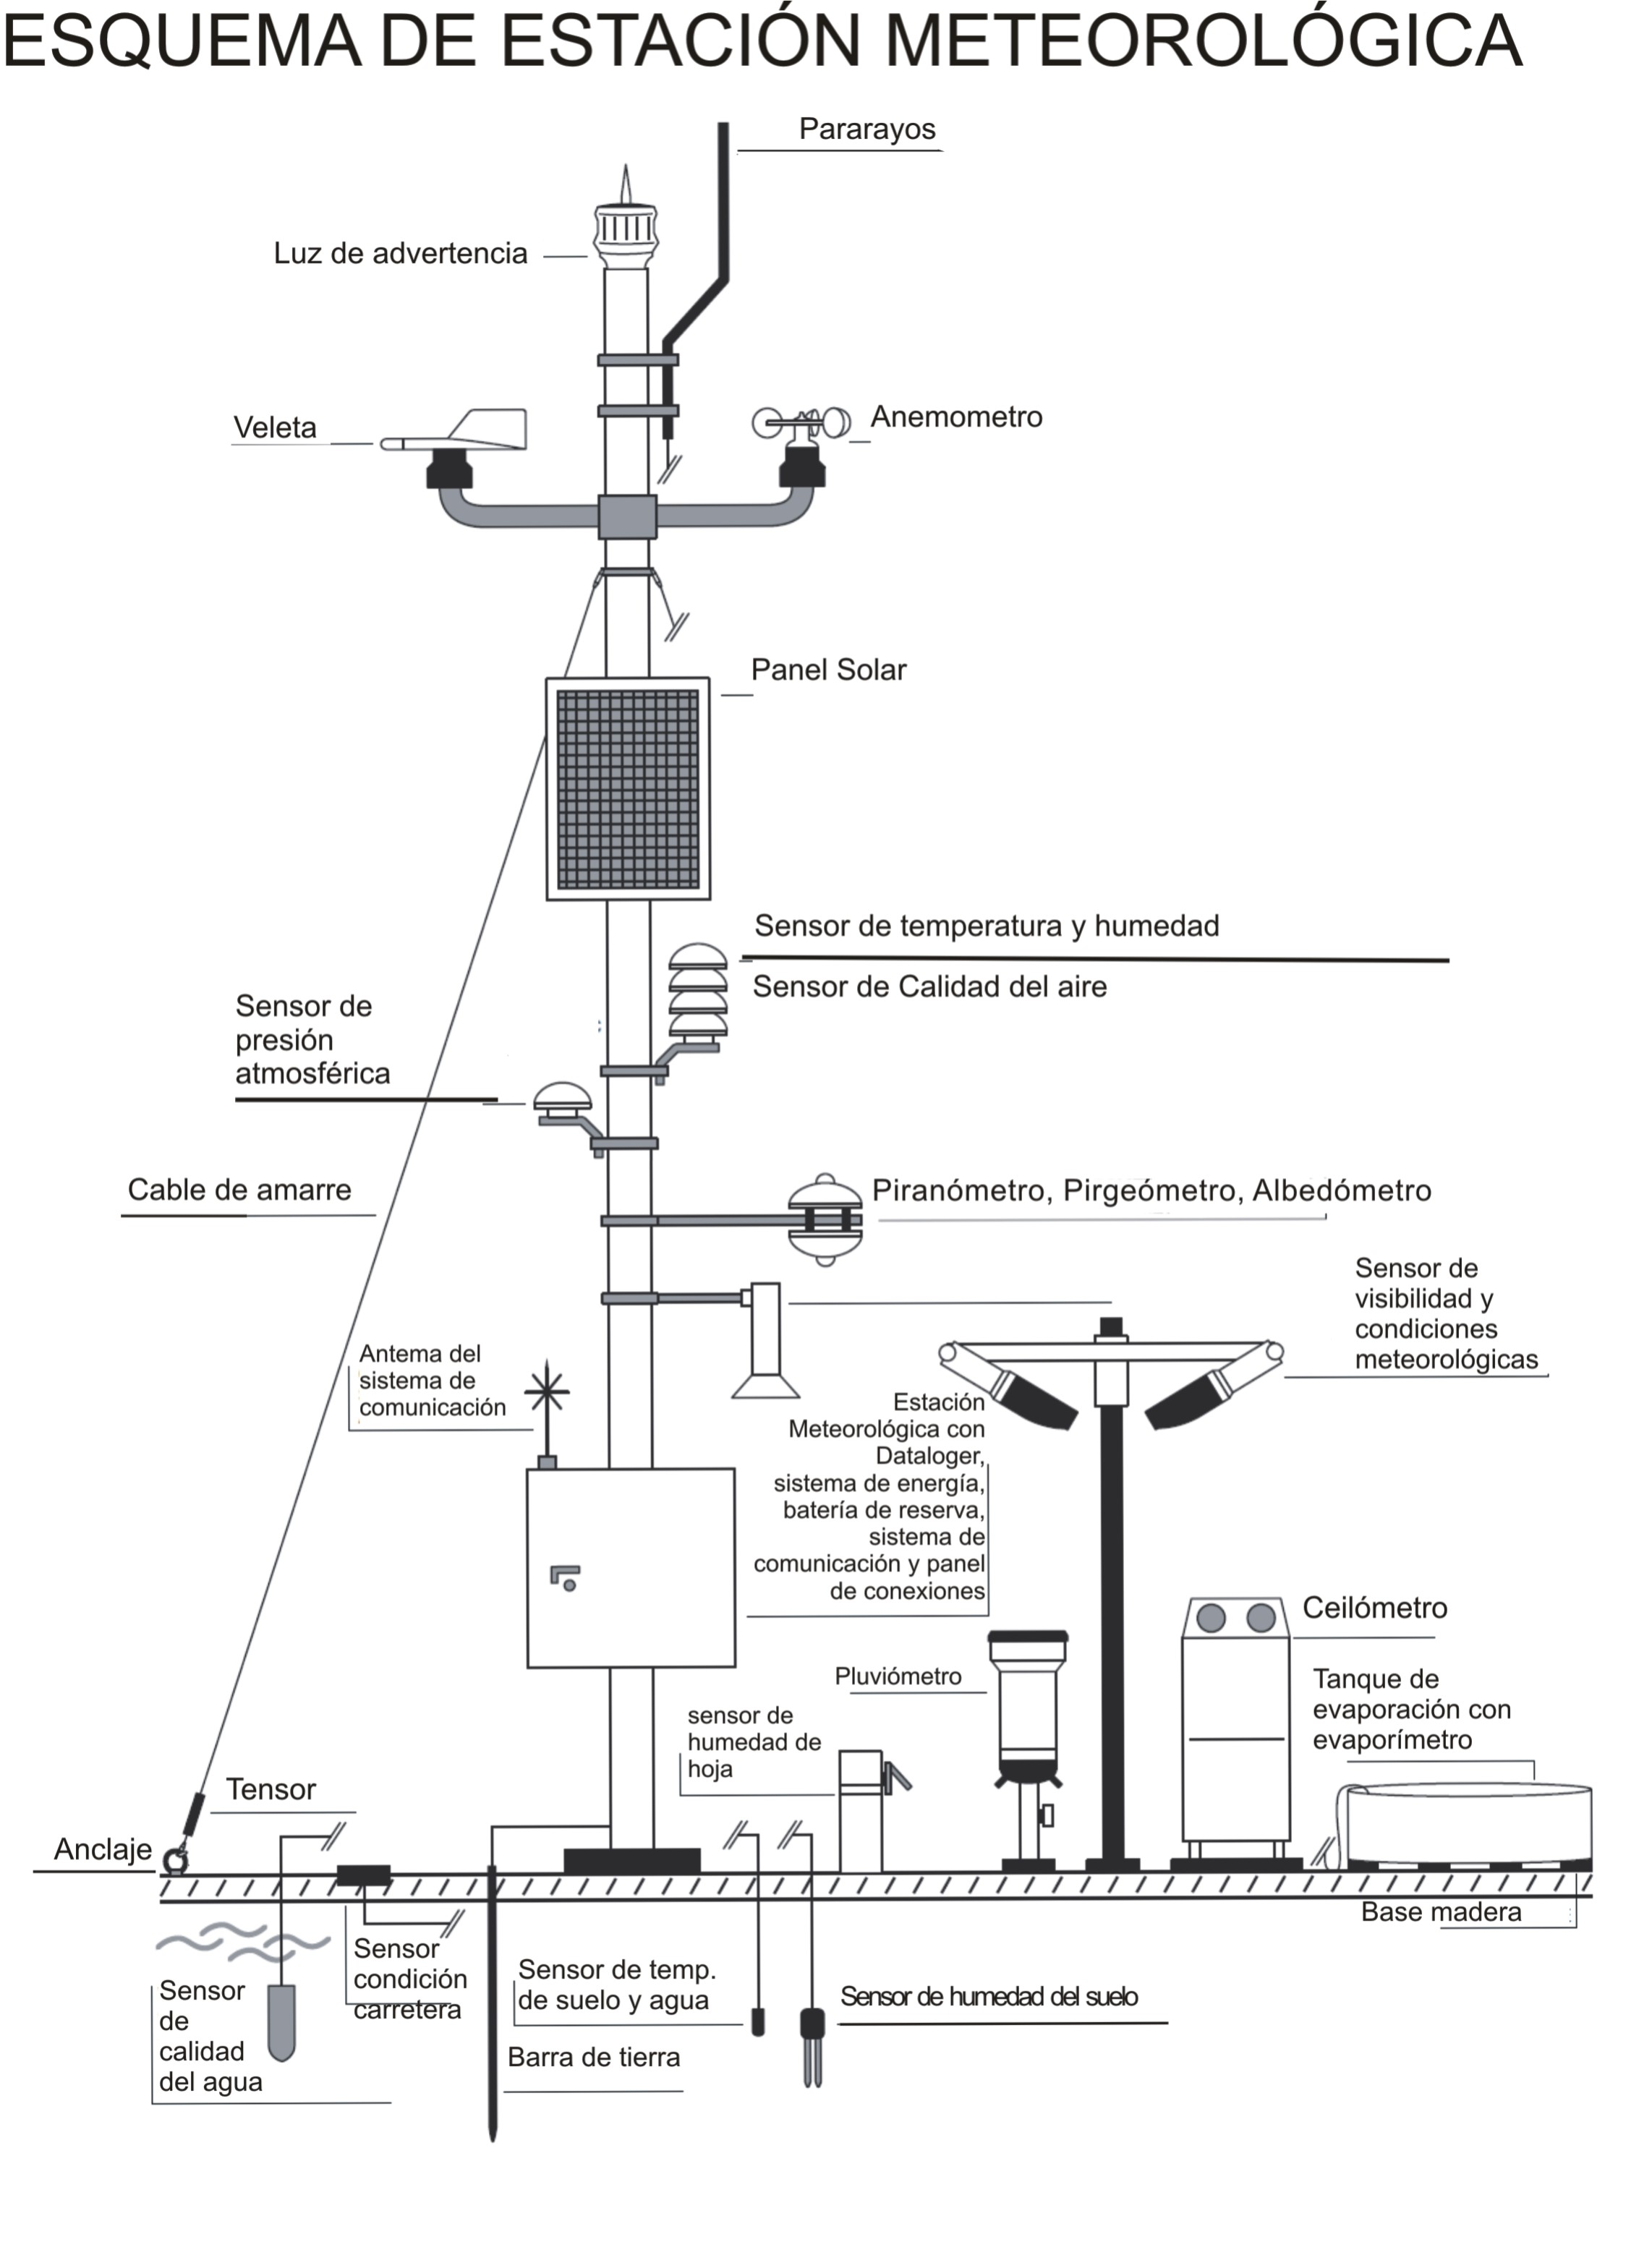
\includegraphics[width=0.5\textwidth]{ma1.jpg}
  \caption{Partes de una estación meteorológica compacta}
  \label{ma1}
\end{figure}

\begin{definition}[Estación metereológica]
    Es un área representativa de una región dotada de equipo meteorológico convencional o automático, en la que se: observan, miden, registran, concentran y procesan los diferentes elementos del tiempo o del clima
\end{definition}

Según su finalidad, se puede clasificar en:
\begin{itemize}
    \item Sinópticas
    \item Climatológicas
    \item Agrícolas
    \item Especiales
    \item Aeronáuticas
\end{itemize}

Así como de acuerdo a la magnitud de las observaciones
\begin{itemize}
    \item Principales
    \item Ordinarias
    \item Adicionlaes: Transitorias y operacionales
\end{itemize}

Por el nivel de observación:
\begin{itemize}
    \item Superficie
    \item Altitud
\end{itemize}

Sinópticas

\begin{itemize}
    \item Superficie \begin{itemize}
        \item Terrestres \begin{itemize}
            \item Dotadas de personal automáticas \begin{itemize}
                \item Principales
                \item Suplementarias
            \end{itemize}
        \end{itemize}
        \item Marítimas \begin{itemize}
            \item Dotas de personal \begin{itemize}
                \item Fijas \begin{enumerate}
                    \item Buqes fijos
                    \item Buqes faros
                \end{enumerate}
                \item Móviles \begin{enumerate}
                    \item Buqes móviles
                    \item Buqes seleccionados
                \end{enumerate}
            \end{itemize}
            \item Automáticas \begin{itemize}
                \item Fijas \begin{enumerate}
                    \item En aguas poco profundas
                    \item Ancladas
                    \item Buque faro
                \end{enumerate}
                \item Móviles\begin{enumerate}
                    \item Boyas a la deriva
                    \item Hielo flotante
                    \item Buques
                \end{enumerate}
            \end{itemize}
        \end{itemize}
    \end{itemize}
      \end{itemize}

\begin{definition}[Estación climatológica]
    Es un grupo o conjunto de instrumentos convencionales o automáticos, en un área con ciertas características, para medir microclima particular, usualmente seleccionado como representativo de una región
\end{definition}

\begin{itemize}
    \item Principales
    \item Referencia
    \item Pluviométricas
    \item Radiométricas
    \item Evaporimétricas
    \item Fines especiales
\end{itemize}

Agrícolas:
\begin{itemize}
    \item principales
    \item ordinarias
    \item Adicionales
    \item Fines especiales
\end{itemize}

Fines especiales:
\begin{itemize}
    \item Observaciones de parásitos atmosféricos
    \item Electricidad atmosféricas
    \item Localización con radar de hidrometeoro y nubes
    \item Hidrológicas
    \item Contaminación atmosférica
    \item Medida de ozono
    \item Microclimatológicas
    \item Química atmosférica
\end{itemize}


Descripción general de las estaciones meteorológicas

Según finalidad general:

\textbf{Sinópticas:} Permiten conocer en una amplia región el estado de la atmósfera en un momento determinado y hacer pronóstico de su evolución y comportamiento.

\textbf{Climatológicas:} Son estaciones que miden datos meteorológicos con una consistencia, homogeneidad y duración, que permiten determinar el clima de una región

Descripción general de las estaciones meteorológicas:

\textbf{Agrícolas o agrometeorológicas:} Son estaciones que proporcionan datos meteorológicos, biológicos y fenológicos, útiles en la determinación de los efectos del tiempo y el clima en el proceso evolutivo de las plantas, para estudiar las mejores condiciones para su adaptación y óptima producción

\textbf{Especiales:} Son estaciones establecidas con carácter temporal o permanente para la medición, observación y procesamiento de uno o varios elementos

\textbf{Aeronáuticas:} Están destinadas a efectuar observaciones meteorológicas en superficie como en altura para proporcionar información sobre el estado del tiempo atmosférico, su comportamiento y evolución para servicio de la navegación aérea

\textbf{Satélites meteorológicos:} Son plataformas colocadas en orbita terrestre, desde las cuales se toman fotografías a gran escala de la atmósfera y la superficie terrestre para conocer el comportamiento y evolución de los elementos meteorológicos.

Según la magnitud de sus observaciones (información) que suministran:

\textbf{Principales:} Estas estaciones están dotadas con casi todos los instrumentos meteorológicos y determinan las condiciones generales del clima de una región

\textbf{Ordinarias:} Determinan las condiciones climáticas locales o características especiales de uno o varios elementos.

A estas dos se les confiere la categoría de referencia, cuando su entorno no cambia durante muchos años

\textbf{Auxiliares o adicionales:} éstas surgen de la necesidad de información específica en lugares no cubiertos por las estaciones principales u ordinarias. Según sus características se distinguen dos clases:

\textbf{Transitorias:} Son de uso inmediato y temporal y toman datos de fenómenos meteorológicos que afectan a los cultivos o crean las condiciones propicias para el desarrollo de plagas o enfermedades

\textbf{Operacionales:} Son de carácter permanente o hasta cuando se tiene un cambio en el sistema de operación, proveen datos específicos para abastecimiento y contaminación de agua, control de embalses y previsión de crecientes.

\subsubsection{Criterios para establecer una estación}

La densidad de una red se determina a partir del área de establecimiento de ésta. Desde el punto de vista teórico, si se quisiera saber cuántas estaciones se necesitan en el país, se parte de su área y de suponer una red de un lado conocido, para lo cual se utiliza la relación:
\begin{equation}
    NE= \frac{Ae}{Ac}
\end{equation}
Donde $NE$ es el número de estaciones, $Ae$ es el área de establecimiento y $Ac$ es el área del cuadrado.

Con la siguiente expresión, se puede determina el número mínimo de estaciones $NME$ conociendo el área de establecimiento en $Km^2$ (A):
\begin{equation}
    NME = \frac{\sqrt{A}}{3} 
\end{equation}
Para propósitos hidrometereológicos, Linsley recomienda las siguientes densidades mínimas: 
\begin{itemize}
    \item Para zonas planas en regiones tropicales mediterráneas o templadas una estación por cada 600 a 900 $km^2$
    \item Para zonas montañosas en regiones tropicales, mediterráneas o templadas una estación por cada 100 a $250km^2$
    \item Para zonas áridas una estación por cada 1500 a $10,000 Km^2$
\end{itemize}
La organización meteorológica mundial propone una gráfica con diferentes líneas, con las cuales se calcula la cantidad mínima de pluviógrafos necesarios para determinar la precipitación media anual.

\begin{table}[h!]
    \centering
    \begin{tabular}{@{}llll@{}}
    \toprule
    \multirow{2}{*}{\begin{tabular}[c]{@{}l@{}}Escurrimiento medio\\ anual en cm/año\end{tabular}} & \multicolumn{3}{l}{\begin{tabular}[c]{@{}l@{}}Días de tormenta\\ por año\end{tabular}} \\ \cmidrule(l){2-4} 
                                                                                                   & <30                        & 30-45                        & >45                        \\ \cmidrule(r){1-1}
    >15                                                                                            & 1                          & 2                            & 3                          \\
    $\leq 15$                                                                                      & 2                          & 3                            & 4                          \\ \bottomrule
    \end{tabular}
    \caption{Escurrimiento en cm/año}
    \label{tabma1}
\end{table}
\begin{figure}[h!]
\centering
  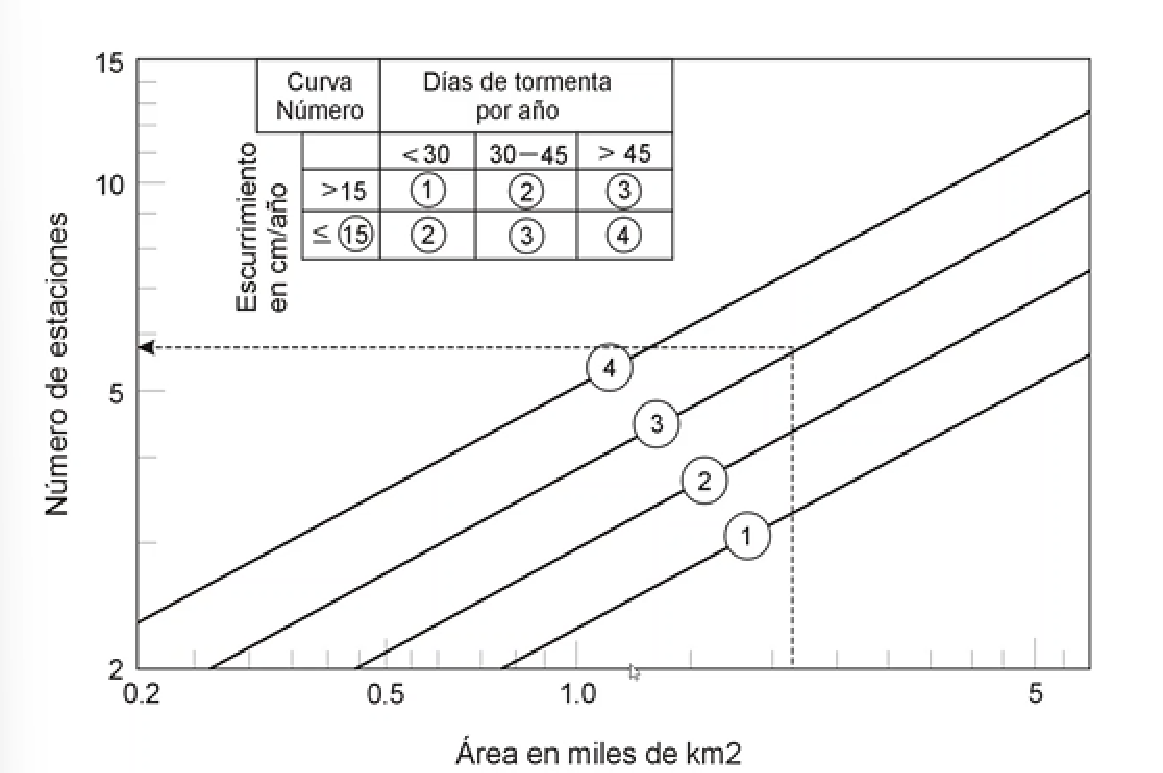
\includegraphics[width=0.5\textwidth]{ma2.pdf}
  \caption{Área de establecimiento}
  \label{ma2}
\end{figure}

A partir de la información de una red de estaciones meteorológicas, se puede definir la distancia entre una estación base con algúna estación secundaria.

El segundo criterio es la ubicación (Tanto en forma general) son para cuando el área se va a establecer la red de un país, estado o región.
\begin{itemize}
    \item \textbf{Los factores geográficos}, es necesario considerar la cercanía al mar y en áreas continentales la cercanía a cuerpos de aguas.
    \item \textbf{Cuencas hidrológicas}, se puede considerar como la unidad de estudio, debido a las variaciones y se requiere de la buena delimitació.
    \item \textbf{Vegetación natural}, delimtar las áreas representativas en que se desarrollan los diferentes tipos de vegetación natural
    \item \textbf{Cultivos}, se deben omar en cuenta las áreas donde predomina un cierto cultivo
    \item \textbf{Zona urbana}, éstas modifican el comportamiento de los elementos metereológicos
\end{itemize}
Un criterio importante es la representividad, así como el emplazamiento despejado no deben existir obstaculos naturales o artificiales; El terreno seleccionado para la estación no deberá presentar depresiones, ya que ésto ocasionaría problemas en la época lluviosa como inundaciones y el acceso a la toma de observaciones. También focos de aire frío, por lo cuál deberá estar nivelado; La cercanía del observador es importante porque se requiere tomar datos manualmente; Que sea de fácil acceso, tanto para la instalación; 

\subsubsection{La observación metereológica}

Consiste en la medición, cuantificación y observación de todos los elementos del tiempo atmosférico que en su conjunto caracterizan el estado atmosférico en un momento dado y en un lugar determinado, se utiliza adecuado, instrumental se complementa con la observación de los sentidos, principalmente la vista.

Estas observaciones se realizan con métodos en forma sistemática, uniforme, ininterrumpida y a horas establecidas y en el menor tiempo posible.

\begin{definition}[Instrumento metereológico]
    Es un dispositivo diseñado y construido para cuantificar el valor del elemento que caracteriza físicamente al fenómeno natural, cuando tal valor no puede ser determinado directamente por los sentidos del hombre
\end{definition}

Todo instrumento debe estar esencialmente dotado de una parte que reaccione a los efectos inducidos por el elemento que ha de medirse y de otra donde, la respuesta o reacción sea convertida en señales fácilmente perceptibles con nuestros sentidos. A la primera se le denomina elemento sensible y a la segunda escala

\begin{itemize}
    \item \textbf{Precisión}: Es la diferencia o relación que existe entre el valor del instrumento patrón y el convencional, se considera como un término de error
    \item \textbf{Sensibilidad}: Es el nivel de detalle que suministra el instrumento para realizar la lectura, por ejemplo en un termómetro: $0.01^{\circ}C, 0.1^{\circ}C, 0.5^{\circ}C, 1^{\circ}C$.
    \item \textbf{Solidez}: Es con respecto a la construcción del aparato y debe ser tal que permita resistir los embates del manipuleo, transporte y la intemperie
    \item \textbf{Simplicidad}: En el diseño debe manifestarse en la operatividad como en el mantenimiento del instrumento
\end{itemize}

\subsubsection{Clasificación del intrumental}

\begin{figure}[h!]
\centering
  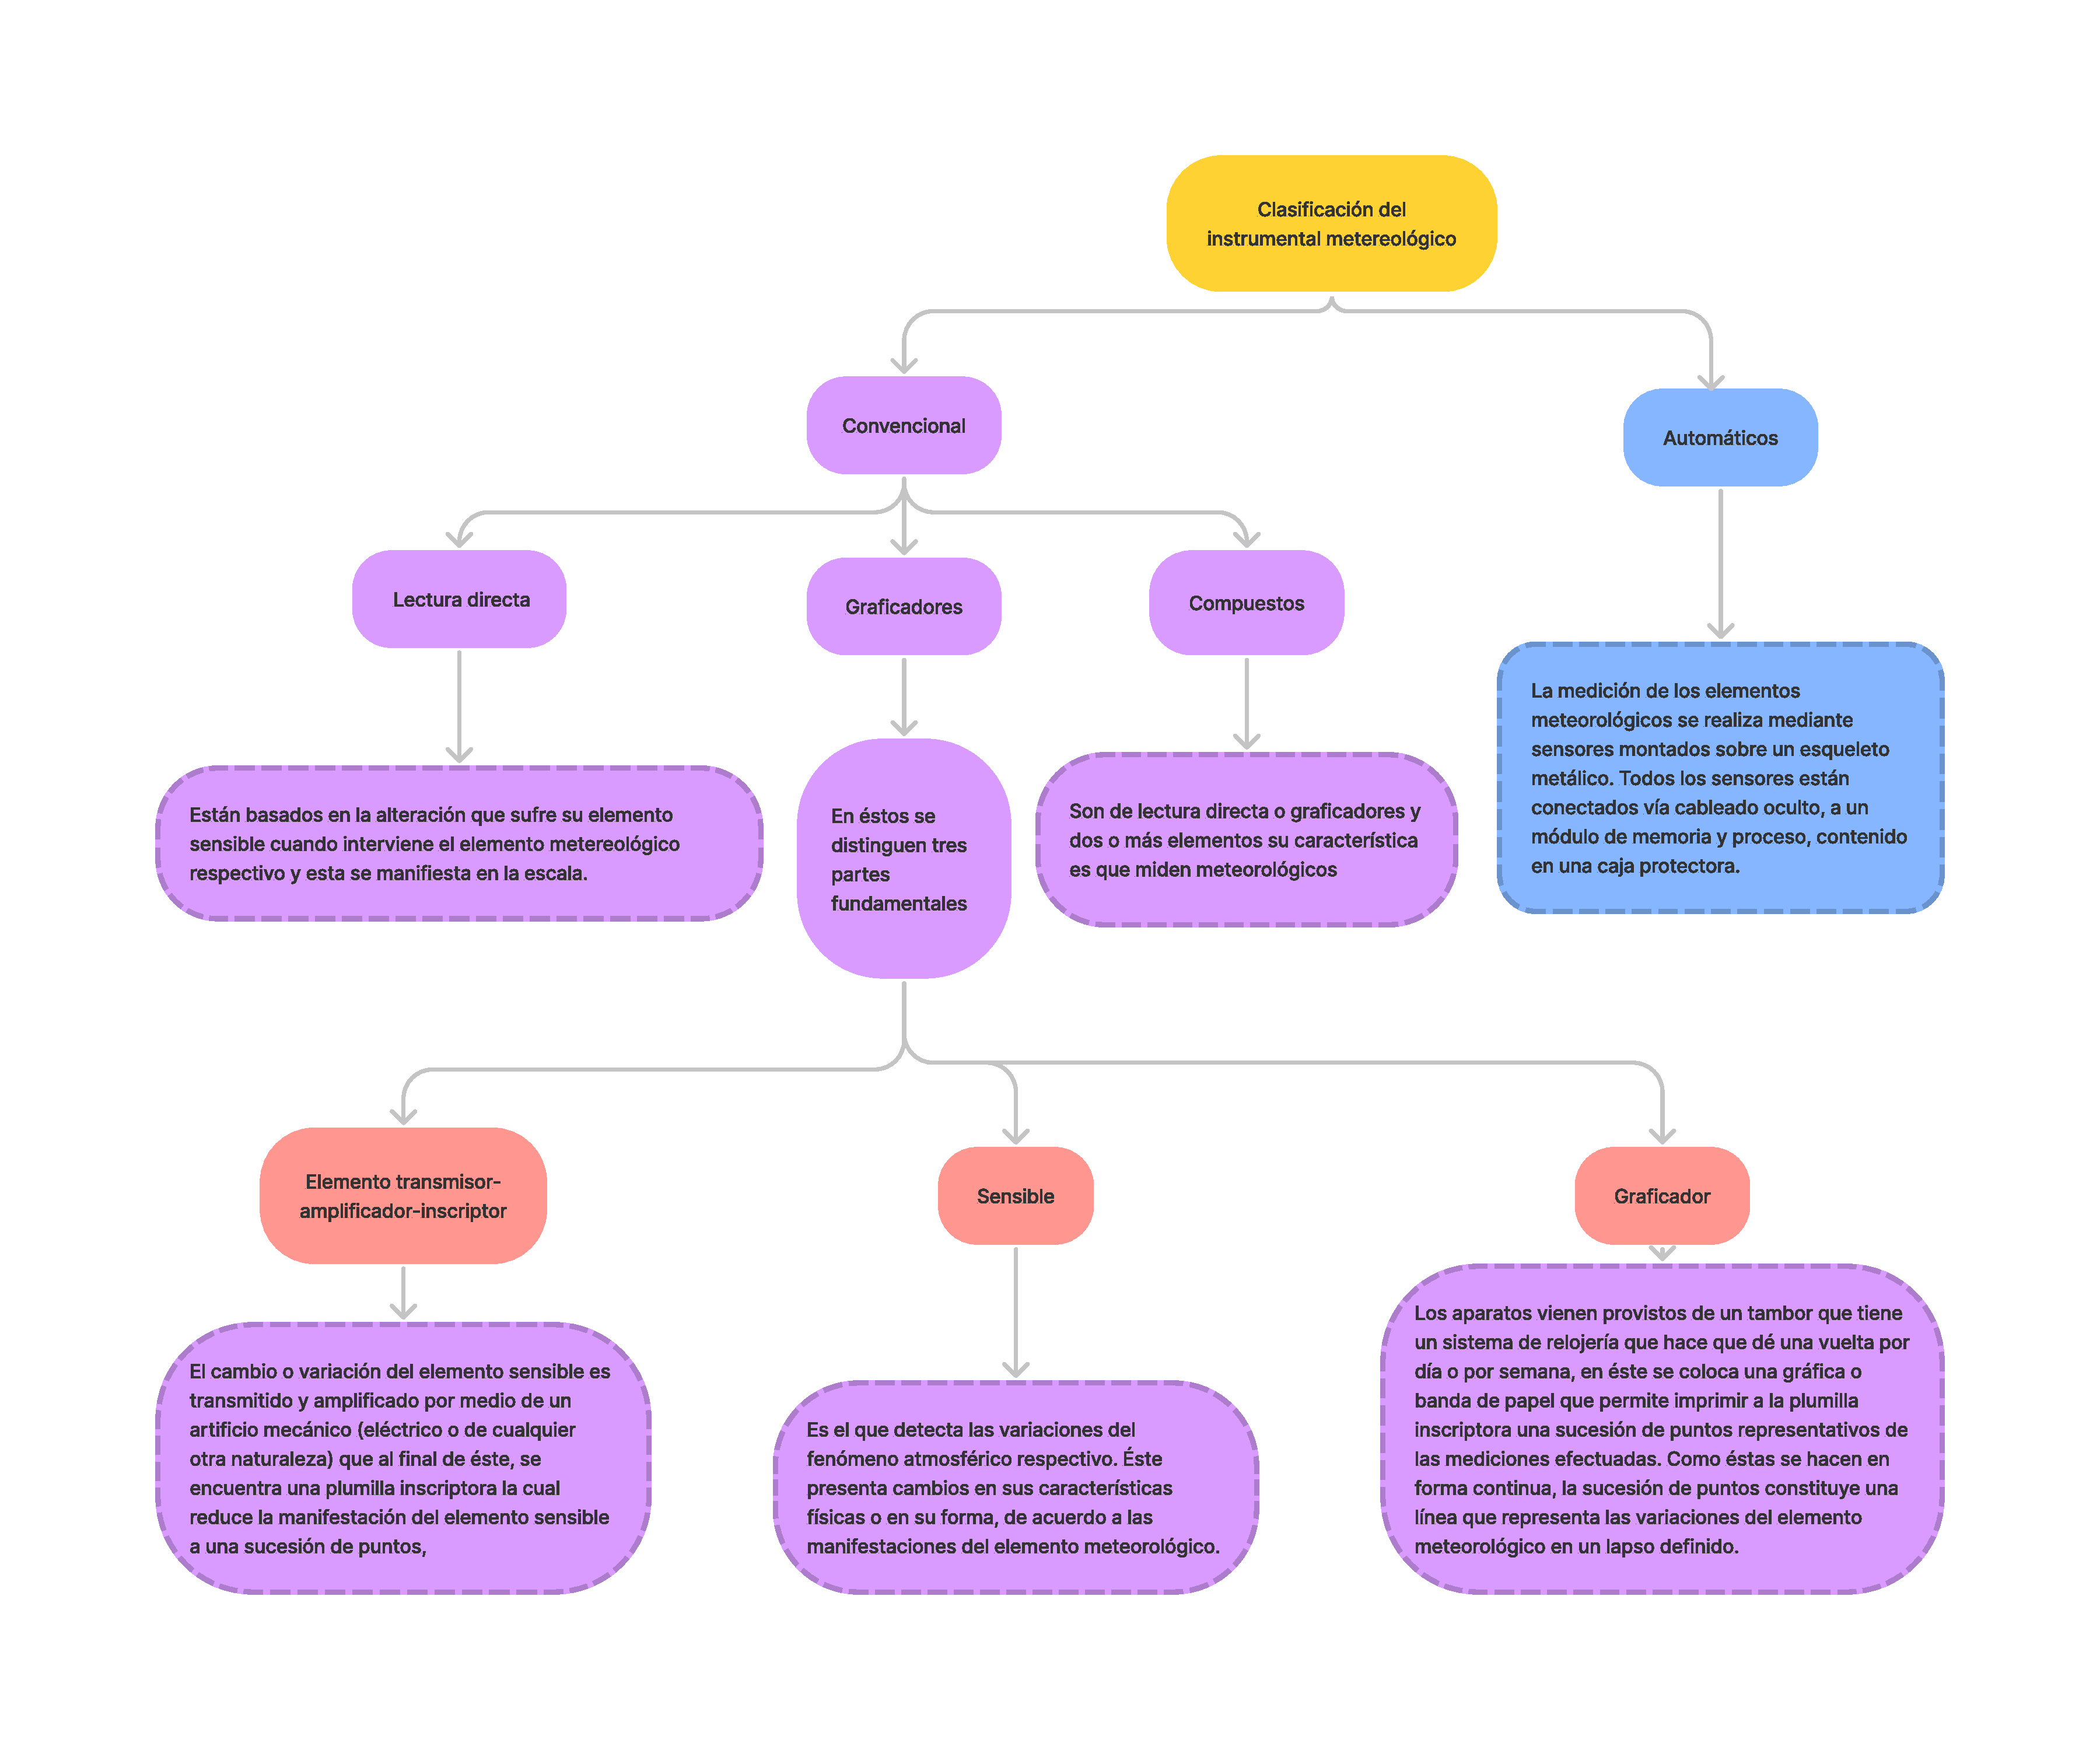
\includegraphics[width=1\textwidth]{ma6.pdf}
  \caption{Clasificación de los instrumentos meteorológicos}
  \label{ma6}
\end{figure}

Como la lluvia llena un lado de balancín, el Peso del agua hace que el balancín se incline y tire su contenido. Al inclinarse el balancín el imán fijo, pasa por el imán estacionario y genera el envío de una corriente al transmisor de a bajo.
\subsubsection{Caseta}

El objetivo de las  observaciones meteorológicas, es contar con datos cuantitativos que representen las condiciones del aire libre.

Cuando se coloca un termómetro a la interperie y recibe directamente los rayos del sol, aumentará su temperatura, por lo que el termómetro marcara su propia temperatura y no la del aire.

La Finalidad de la caseta es evitar que sobre los instrumentos colocados en su interior actúen elementos que alteren las mediciones de éstos.

\textbf{Acondicionamiento:} Las paredes deben ser dobles y están provistas de celosías, a manera de persianas, que permiten la libre circulación del aire.
    \begin{figure}[h!]
    \centering
      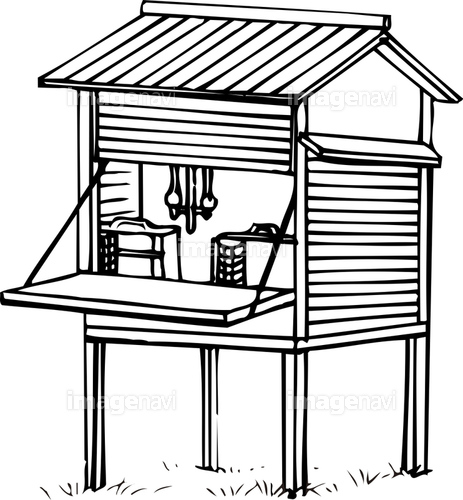
\includegraphics[width=0.5\textwidth]{ma3.jpg}
      \caption{caseta}
      \label{ma3}
    \end{figure}
Este generalmente es de madera o cualquier material aislante y ligero se pinta de blanco a fin de que absorba lo menos posible los rayos solares

\section{Modelos matemáticos en la agricultura}

Es la representación de un fenómeno real basado en relaciones matemáticas:
\begin{equation}
  R_n = H + H + LE\implies \underbrace{LE}{ET} - R_n = \underbrace{H}{Ts - Ta}
  \label{eqevapo}
\end{equation}
La ecuación \eqref{eqevapo} describe la evapotranspiración: Son fórmulas, gráficas o tablas que describen el comportamiento de un sistema real.
\begin{itemize}
  \item Así mismo, es un bosquejo que representa un conjunto real con cierto grafo de precisión y en la forma más completa posible, pero sin pretender aportar una réplica de lo que existe en la realidad.
  \item Puede ser una representación simplificada de un sistema delimitada del mundo real,
  \item Representación de una parte de un sistema real, que conceptualiza las interrelaciones y respuestas de las condiciones de este y que es capaz de hacer pronósticos bajo un conjunto de condiciones propuestas (Rabadan y Guitron, 2012)  
\end{itemize}

Las razones por la que se modela son:
\begin{enumerate}
  \item Permite realizar en corto tiempo estudios a largo plazo
  \item Admite la repetición, de un evento que ocurriría solamente una vez en el sistema real
  \item A partir de éstos se puede estimar la probabilidad de que un evento ocurra
  \item Con ellos se puede hacer experimentación controlada en situaciones donde no es posible realizarla físicamente o el costo de hacerla es muy alto o ambos
  \item Se puede tener un aprendizaje profundo de las relaciones internas y externas y del funcionamiento del sistema
\end{enumerate}

En el caso de un modelo agrometereológico, éste se da en relaciones complejas:
\begin{itemize}
  \item Tiempo atmosférico \begin{itemize}
    \item Clima
  \end{itemize}
  \item Desarrollo \begin{itemize}
    \item Crecimiento
    \item Rendimiento
    \item Componentes del rendimiento
  \end{itemize}
  \item Métodos\begin{itemize}
    \item Matemáticos
    \item Estadísticos
  \end{itemize}
\end{itemize}

Los criterios para la clasificación de los modelos agrometeorológicos son 

El origen de los datos; El planteamiento (diseño) predominante del problema; El fin (solución) del modelo; Su aplicación potencial

Considerando los criterios anteriores los modelos agrometeorológicos se clasifican en: Simulación del crecimiento de los cultivo (mecanicistas) (MSC); Análisis del crecimiento de los cultivos (MAC); Estadísticos - Empíricos (ME-E).

La simulación del crecimiento de los cultivos (MSC), consiste en los elementos como la radiación, temperatura, humedad atmosférica y el viento, al mismo tiempo que los procesos consisten en la fotosíntesis, respiración y transpiración.
Está simulada mediante ecuaciones matemáticas e integraciones con lenguajes de programación.

Para el análisis del crecimiento de los cultivos, se tiene que tomar en cuenta la precipitación, evaporación, capacidad de almacenamiento del suelo, humedad del suelo, evapotranspiración, desarrollo morfológico, crecimiento vegetal y el rendimiento. Ésta se da con técnicas convencionales estadísticas

Los estadísticos empíricos: Su planteamiento no conduce fácilmente a una explicación causa-efecto
Se toman en cuenta los datos meteorológicos, Datos de suelo, Rendimiento de un cultivo, Datos de manejo, Simulación del rendimiento: Métodos estadísticos: Funciones de producción; \texttt{Son validas para la región o lugar donde se generan}.

Fin de los modelos agrometeorológicos:
\begin{enumerate}
  \item MSC: Son elementos básicos de la investigación, para estudiar los procesos específicos de las plantas como una respuesta al medio ambiente. Tienen la habilidad de reproducir importantes procesos físicos, químicos o biológicos y describir cómo y porqué resulta una respuesta particular
  \item MAC: Son medios prácticos de investigación para el análisis de las variaciones del rendimiento final en función de las contribuciones y las variaciones de cada una de las variables del tiempo o el clima
  \item ME-E: Son para pronosticar y conocer la variabilidad del rendimiento de los cultivos en una región dada en función de los elementos del clima. Son descriptivos, se derivan de datos observados de uno o más ciclos de cultivo, no involucran procesos fisiológicos y tienen escasa capacidad explicativa.
\end{enumerate}
Las aplicaciones de los modelos son:
\begin{enumerate}
  \item Estudios de fisiología y morfología de cultivos, Ingeniería genética de cultivos, estrategias de manejo de cultivos
  \item MAC: Pronóstico del desarrollo, madurez y rendimiento de los cultivos, manejo del agua en riego
  \item ME-E: Zonificación agroclimática de cultivos, Estimación del impacto climático en el rendimiento de los cultivos,
\end{enumerate}
\begin{figure}[h!]
\centering
  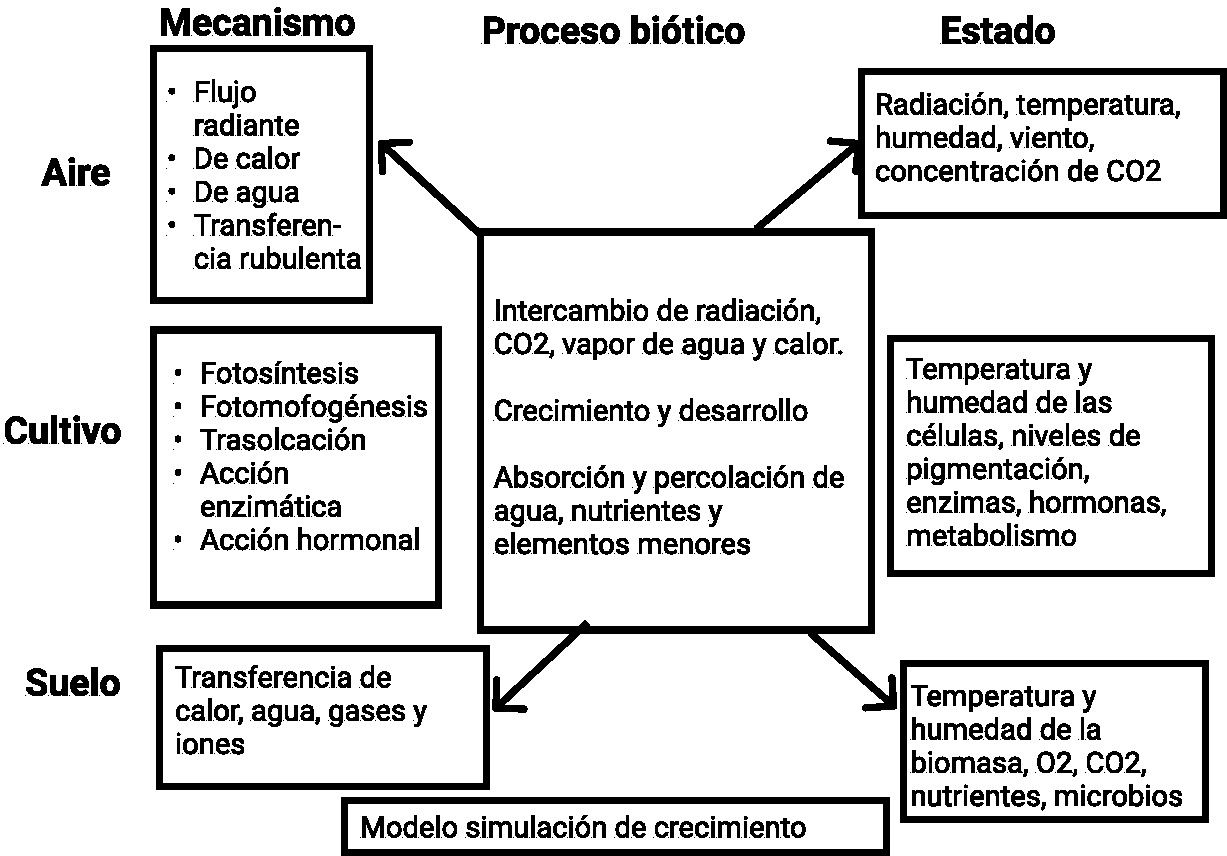
\includegraphics[width=0.5\textwidth]{ma4.pdf}
  \caption{Módelo de simulación del crecimiento}
  \label{ma4}
\end{figure}
\begin{figure}[h!]
\centering
  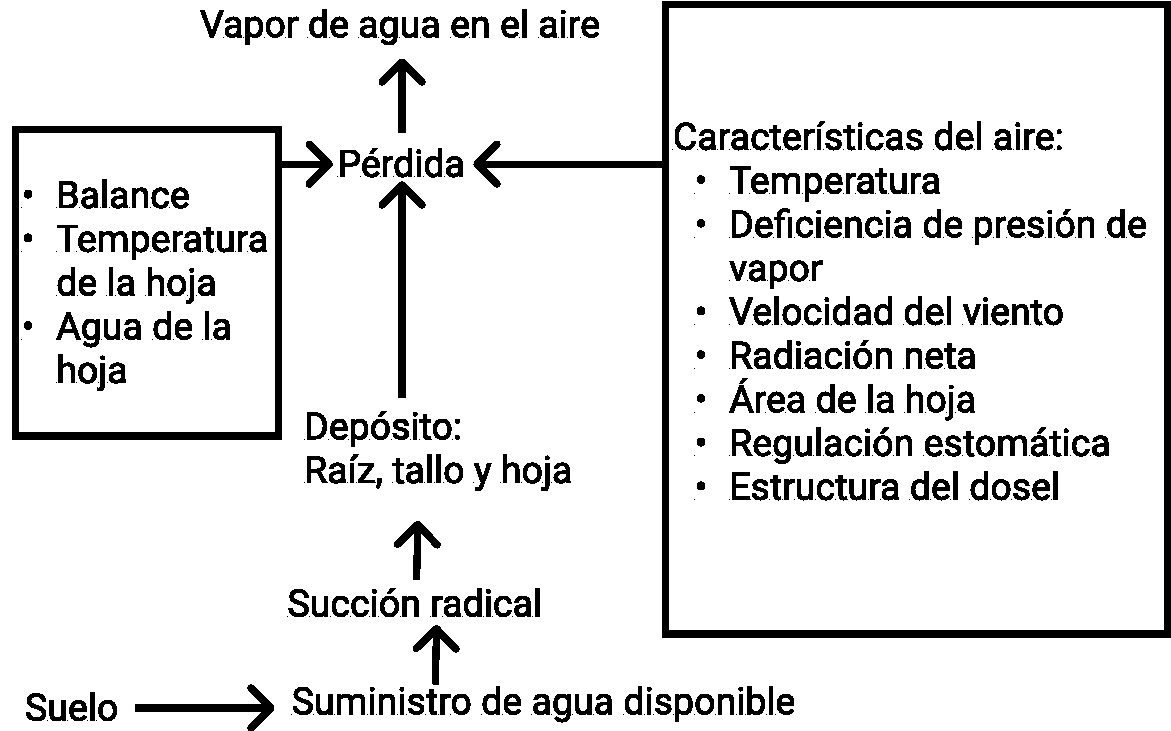
\includegraphics[width=0.5\textwidth]{ma5.pdf}
  \caption{Modelo de análisis del crecimiento}
  \label{ma5}
\end{figure}
\subsection{Métodos estadísticos empíricos}
Puede usarse una regresión lineal simple, el cuál se refiere a un conjunto de pares de valores en un experimento de x,y; se realiza un diagrama de dispersión entre las variables; así mismo es muy importante aplicar el método de mínimos cuadrados, con las siguientes expresiones matemáticas:
\begin{align*}
    &\bar{x} = \frac{\sum x_i}{N}\\
    &\bar{y} = \frac{\sum y_i}{N}\\
    &SC_x = \sum x_i^2 - \frac{\left(\sum x_i\right)^2}{N}\\
    &SC_y = \sum y_i^2 - \frac{\left(\sum y_i\right)^2}{N}\\
    &SC_{xy} = \sum xy_i^2 - \frac{\left(\sum xy_i\right)^2}{N}\\
    &\hat{b} = \frac{SC_{xy}}{SC_x}\quad \text{Pendiente}   \\ 
    &\hat{a} = Y - \hat{b}X\quad \text{Parámetro de posición} \\
    &r^2 = \frac{\left(SC_{xy}\right)^2}{SC_x\cdot SC_y}\quad \text{Coeficiente de determinación}
\end{align*}
\subsubsection{Exponencial}
Se tienen varais expresiones, se presentan tres
\begin{align}
    &y = ab^x\\
    &y = ae^{bx}\\
    &y = e^{\left(a + bx\right)}
\end{align}

De la transformación $Y=ab^x$, se toman los logaritmos neperianos $\ln{(a)}=\ln{(Y)}+X\ln{(b)}$
Quedando la expresión
\begin{equation}
    Y_t = a_t + b_tX
\end{equation}
Análogamente, de la expresión $\ln{(Y)}=\ln{(a)}+X\ln{(b)}$
\begin{equation}
    Y_t =a_t + b_tX
\end{equation}

\subsubsection{Saturación}
Se defina como cualquiera de las siguientes modelos:
\begin{align*}
    &y = \frac{ax}{b + x}\\
    &\frac{1}{y} = \frac{b + x}{ax}\\
    &\frac{1}{y} = \frac{b}{ax} + \frac{1}{a}\\
\end{align*}
LLegando a la expresión|
\begin{equation}
    Y_t = a_t + b_tX_t
\end{equation}

En el caso de una regresión lineal por transformación (Modelo no lineal), se presentan seis modelos no lineales:
\begin{itemize}
    \item Potencial
    \item Exponencial
    \item Saturación
    \item Analógico de Hollings
    \item Logística
    \item Normal
\end{itemize}

\subsubsection{Potencial}

Se toman logaritmos naturales
\begin{equation}
    y = ax^b
\end{equation}
Y se denotan nuevas variables de la fórmula $\ln{Y}=a\ln{(a)}+b\ln{(X)}$
\begin{align*}
    Y_t =\ln{(Y)}&&a_t=\ln{(a)}&&X_t=\ln{(X)}&&b_t = b
\end{align*}
Así llegamos a la expresión:
\begin{equation}
    Y_t = a_t + X_t
\end{equation}

\subsubsection{Analógico de Hollings}

\begin{align*}
    &Y = \frac{X}{a + bX}&&Y_t = \frac{X}{Y} + a_t = a_tb_t = b_tX_t = X\\
    &Y\left(a + bX\right) = X&& Y_t = a_t + b_tX_t\\
    &\frac{X}{Y} - a = bX&&
\end{align*}
\subsubsection{Transformación Logística}

\begin{align*}
    &y = \frac{k}{1 + e^{a + bx}}&& \frac{k}{y} - 1 = e^{a1bx} &&at = a\\
    &\frac{1}{y} = \frac{1 + e^{a + bx}}{k}&& \ln{\left(\frac{k}{y} - 1\right)}= a+ bx&&b_t = b\\
    &\frac{k}{y} = 1 + e^{a + bx}&&X_t = x&&Y_t =\ln{\left(\frac{k}{y} -1\right)}
\end{align*}
\subsubsection{Transformación normal}

\begin{equation}
    text {Logistica por el origen}\quad Y = K\left(1 + e^{bx}\right)
\end{equation}

Se puede expresar como:
\begin{align*}
    &\frac{Y}{K} = 1 - e^{-bx}\\
    &\frac{Y}{K} - 1 = e^{-bx}\\
    &1 - \frac{Y}{K} = e^{-bx}\\
    &\ln{\left(1 - \frac{Y}{K} \right)} = e^{bx}    \ln
\end{align*}

$Y_t=\ln{\left(1- \frac{Y}{K} \right)}$

Por lo tanto el modelo original estará dado por las tres ecuaciones siguientes:
\begin{align}
    &y = ae^{\frac{\left(x - x_0\right)^2}{b^2}} && x_t =\left(x - x_0 \right)^2\\
    &\ln{(y)} =\ln{(a)} + \frac{\left(x - x_0\right)^2}{b^2}&&b_t = \frac{1}{b^2}\\
    &\ln{(y)} =\ln{(a)} + \frac{\left(X - X_0\right)^2}{b^2}&&y_t = \ln{(y)} -\ln{(a)}\\
    &Y_t = b_tX_t
\end{align}

\section{Fenología}
Existen características cuantitativas (que se pueden medir) y morfológicas (que se pueden observar). Uno de los fenómenos naturales más evidente es que las plantas aumenten de tamaño en forma más o menos continua y desarrollen nuevos órganos en forma intermitente durante su ciclo de vida

En la vida de un vegetal se distinguen dos grandes reacciones o etapas:

El \textbf{crecimiento}, que es el incremento en tamaño, peso o área de las partes de una planta,

El \textbf{desarrollo}, que es el paso O cambio de las partes de una planta a través de aspectos morfológicos diferentes sucesivos.

Las reacciones de las plantas, depende de una interacción coordinada con el ambiente, material genético y el hombre; sobre los procesos fisiológicos internos se manifiestan en el crecimiento y desarrollo de los vegetales haciéndose evidentes por medio de los fenómenos periódicos de los vegetales ésto por la preencia de las primeras hojas, brotación de yemas, floración, formación del fruto, su maduración y la caída de las hojas.

El objetico de la fenología vegetal, es el estudio de las relaciones entre los elementos atmosféricos y los fenómenos periódicos de los vegetales, relacionándose con la fisiología, ecología, meteorología y climatología; agricultura, ganadería, silvicultura y conservación de la naturaleza (actividad del sector agrario)

\begin{definition}[Fenología]
    Es la ciencia que estudia los fenómenos periódicos de los vegetales y su relación con el tiempo atmosférico (Romo Y Arteaga, 1987)
\end{definition}

Tiene como estudio determinar las fechas de inicio y término de algunos importantes eventos fenológicos de las plantas y registrarlos en orden cronológico y en lo posible en diferentes lugares y durante varios años, para determinar las relaciones que tienen con los elementos atmosférico (Arteaga, 1995) del

Es el estudio de la ocurrencia de los eventos biológicos pronosticables y su relación con los cambios bióticos y abióticos (Franquie, 1972)

Estudia la periodicidad de las manifestaciones de los eventos biológicos, las causas de su periodicidad con respecto a fuerzas bióticas y abióticas y la interrelación entre fases de la misma diferentes especies (The US/IBP Phenology commitee, 1972)

Es la ciencia que trata sobre los fenómenos biológicos periódicos con respecto al tiempo atmosférico, especialmente con los cambios estacionales. Los eventos fenológicos son estados de desarrollo de la planta. Desde el punto de vista de un climatólogo, estos fenómenos sirven como base para la interpretación de cambios locales y zonas climáticas y son considerados que integran los efectos de un número de factores bioclimatológicos. La fenología puede ser considerada una rama de la bioclimatología (glosario de términos usados en agrometeorología, edición provisional, 1984)

\subsection{Importancia}

Elaborar planes de trabajos agrícolas según el recurso agroclimático de una región y las necesidades agroclimáticas de los cultivos.

Así que también puede prepararse calendarios para el combate de plagas, enferemedades o malezas de acuerdo a la fenología de éstos con la del cultivo; Zonificación fenoclimática en base los mapas; determinación de lso requerimientos agroclimáticos de las diferentes especies y de sus periodos más sensibles,
modelos agrometeorológicos para definir regiones agrícolas potenciales para varios cultivos; pronósticos de condiciones atmosféricas favorables a las plantas con las observaciones fenológicias de plantas indicadoras; programación de la asistencia técnica en base la fenología de cultivos.

Su importancia radica en el conocimiento que proporciona acerca de las respuestas de los vegetales al tiempo atmosférico y las variaciones de dichas respuestas a lo largo de su vida, esto permite determinar las épocas más sensibles de los cultivos, a los elementos del tiempo atmosférico, durante las cuales se debe fijar la atención con el fin de obtener los máximos beneficios con el mínimo costo

\subsubsection{Periodo vegetativo}

En perennes, caducifolias de latitudes medias, botación de temas florales y fóliales, floración y foliación; formación de frutos hasta maduración; defoliación y reposo

La duración de los eventos fenológicos o fenómenos periódicos de los vegetales es generalmente llamada fase y se define como la presencia (manifestación), transformación o interrupción (suspensión o detención) detención) rápida de los órganos órganos o partes de las plantas

\begin{itemize}
    \item Visibles
    \item Criptofases ( fases ocultas)
\end{itemize}

En un campo con un mismo cultivo, es notorio que una misma fase no se presente en la misma fecha, sino que el fenómeno aparece con diferencias muy notables de una planta a otra, de varios días inclusive. Esto se refiere a variaciones locales para una misma fase en un mismo lugar, pero es obvio que una determinada fase de una especie en particular se manifiesta en fechas distintas para lugares con climas diferentes.

\begin{definition}[Isófana]
    Es una línea que une los puntos donde una fase dada se verifica en la misma una fase dada se verifica en la misma fecha:Es la representación geográfica de los Es la representación geográfica de los fenómenos periódicos (fase) de la vida vegetal
\end{definition}

\textbf{Isófana de siembra}: ésta, evidentemente no representa una fase de desarrollo, sino que es tan solo la base necesaria para que comience el periodo vegetativo. Están claramente subordinadas al elemento térmico, ya que su comportamiento corresponde a las exigencias de latitud y altitud, adaptándose a las situaciones generales de distribución de tierras y mares. También dependen de cómo se presenten las precipitaciones pluviales y otros fenómenos meteorológicos y agrotécnicos

Se sabe que la fecha de siembra es un factor muy importante en la duración del periodo vegetativo y por ende en el rendimiento de los cultivos. Siembras Siembras tardías reducen el ciclo vegetativo y siembras tempranas lo prolongan. Siembras antes o después del periodo óptimo de siembra reducen los rendimientos

\textbf{Isófana de floración o isoante}
La isoante es una línea que une puntos donde la floración de una especie dada sucede en la misma fecha misma fecha; La floración es un fenómeno de fácil observación pero es muy variable su fecha de observación pero es muy variable su fecha de iniciación. El rendimiento de un cultivo está muy relacionado con la floración del mismo pues se relacionado con la floración del mismo, pues se ha encontrado que casi todas las especies tienen un periodo de máxima sensibilidad a los elementos atmosféricos durante la floración o muy cercano a ella.

Conociendo la fecha de floración de un cultivo se toman antici padamente las medidas adecuadas para sortear este periodo periodo y evitar disminuciones disminuciones en el rendimiento.

\textbf{Isófana de madurez fisiológica (Cosecha)}

Es la línea que une puntos donde la madurez fisiológica (cosecha) de una especie o variedad dada se verifica en una misma fecha una misma fecha; La forma y distribución de las isófanas de cosecha dependen, de tres factores principales: régimen térmico, régimen pluviométrico y factores agrotécnicos.

Importancia de las isófanas:
\begin{itemize}
    \item Determinación de la aptitud agroclimática de una región para diversos cultivos
    \item Duración del ciclo del cultivo    
    \item Determinación de la fecha óptima de siembra en función de obtener el máximo rendimiento Época del año en la cual se desarrolla el cultivo
    \item Áreas donde el cultivo presenta su máximo rendimiento
    \item Determinación de la presencia de fenómenos adversos desde la siembra hasta la cosecha
\end{itemize}

\begin{table}[h!]
    \centering
    \begin{tabular}{@{}llllll@{}}
    \toprule
    FS  & FF  & FMF  & Rendi & Plagas & ObsMet \\ \midrule
    S1  & FF1 & FMF1 & R1    & P1     & OM1    \\
    S2  & FF2 & FMF2 & R2    & P2     & OM2    \\
    Si  & FFi & FMFi & RI    & Pi     & OMi    \\
    \dots & \dots & \dots  & \dots   & \dots    & \dots    \\
    Sn  & FFn & FMFn & Rn    & Pn     & OMn    \\ \bottomrule
    \end{tabular}
    \caption{Observaciones en un punto de un cultivo Observaciones en un punto de un cultivo}
    \label{tabma2}
\end{table}

\subsubsection{Ley de Hopkins}

La fecha de presencia o manifestación de un fenómeno de carácter periódico de los vegetales (isófana) en primavera se retrasa retrasa cuatro días por cada grado de aumento en latitud en dirección al polo, por cada cinco grados de longitud longitud hacia el Este y por cada 100 m en altitud. En otoño bajo las mismas condiciones se registra un adelanto de cuatro días


Las desviaciones de esta ley son result dado de los factores locales como cercanía a grandes masas de agua, condiciones condiciones topográficas topográficas y la exposición del relieve; Esta ley resalta resalta la acción de los factores factores climáticos como: latitud, longitud y altura sobre los fenómenos fenómenos periódicos periódicos de los vegetales vegetales; Ésta es muy útil pues permite un correcto trazado trazado de las isófanas isófanias con relativamente relativamente pocos puntos

\begin{definition}[Subperiodo]
    Es el tiempo transcurrido entre dos fases sucesivas. Un subperiodo es una verdadera etapa en la vida de una planta por lo que varios autoresprefieren usar el término ``etapa fenológica'' para referirse al`mismo concepto.
\end{definition}

\begin{table}[h!]
    \centering
    \begin{tabular}{@{}ccc@{}}
    \toprule
    Subperiodo & Intervalo                                                                  & Nombre       \\ \midrule
    Primero    & \begin{tabular}[c]{@{}c@{}}Siembra-Inicio\\ amacollaje\end{tabular}        & Nacencia     \\
    Segundo    & \begin{tabular}[c]{@{}c@{}}Inicio amacollaje-fin\\ amacollaje\end{tabular} & Amacollaje   \\
    Tercero    & \begin{tabular}[c]{@{}c@{}}Fin amacollaje-\\ espigamiento\end{tabular}     & Espigamiento \\
    Cuarto     & \begin{tabular}[c]{@{}c@{}}Espigamiento-\\ madurez\end{tabular}            & Madurez      \\ \bottomrule
    \end{tabular}
    \caption{División del periodo vegetativo en cereales}
    \label{tabma3}
\end{table}

\begin{table}[h!]
    \centering
    \begin{tabular}{@{}lll@{}}
    Código & Etapa               & Descripción              \\
    01     & Siembra             & Siembra en húmedo        \\
    10     & Emergencia          & Aparición de hojas       \\
    20     & 1er entrenudo       & Elongación 1er entrenudo \\
    30     & Banderilla          & Aparición banderilla     \\
    40     & Espgia              & Aparición espiga         \\
    50     & Antesis             & Inicio de antesis        \\
    60     & Formación de grano  & Formación de grano       \\
    70     & Lechoso-masoso      & Grano lechoso masoso     \\
    80     & Madurez Fisiológica & Madurez fisiológica      \\
    90     & Senescencia         & Senescencia             
    \end{tabular}
    \caption{Etapas fenológicas del maíz en base al código decimal}
    \label{tabma4}
\end{table}

Con respecto a un cierto elemento meteorológico, es el intervalo relativamente breve del periodo vegetativo durante el cual la planta presenta su máxima sensibilidad a dicho elemento

Sí se conoce en que épocas se presentan:
\begin{itemize}
    \item Permite tomar las medidas adecuadas como: riegos fertilización, aplicación de plaguicidas, labores culturales
    \item Evitar decrementos en los rendimientos b. Evitar decrementos en los rendimientos
    \item Pronóstico de cosechas
    \item Lucha contra adversidades climáticas
\end{itemize}
\begin{table}[h!]
    \centering
    \begin{tabular}{@{}llllll@{}}
    \toprule
    \multirow{2}{*}{Cultivo} & \multicolumn{3}{l}{Cultivo de campo} & \multicolumn{2}{l}{Hortalizas}                                          \\ \cmidrule(l){2-6} 
                             & DDS        & DCV       & \% CV       & Cultivo   & Fase                                                        \\ \midrule
    Arroz                    & 40         & 120       & 30          & Repollo   & Inicio Repo                                                 \\
    Soya                     & 42         & 125       & 34          & OCra      & 10-15cm alt                                                 \\
    Maíz                     & 49         & 120       & 40          & Ajo       & Inicio bulbo                                                \\
    Cacahuate                & 42         & 105       & 40          & Frijol    & \begin{tabular}[c]{@{}l@{}}Formación\\ follaje\end{tabular} \\
    Frijol                   & 30         & 62        & 48          & Zanahoria & 7-10cm alt                                                  \\
    Cebolla                  & 56         & 95        & 60          & Pepino    & \begin{tabular}[c]{@{}l@{}}Inicio\\ vegetativo\end{tabular} \\
                             &            &           &             & Tomate    & 20-30cm alt                                                 \\ \bottomrule
    \end{tabular}
    \caption{Periodo crítico de competencia de malezas en algunos cultivos}
    \label{tabma5}
\end{table}

\begin{definition}[Equivalente meteorológico]
    Son los valores críticos de exceso o deficiencia (límites) de los elementos que afectan el desarrollo, crecimiento crecimiento y rendimiento rendimiento de los cultivos cultivos. Los EM se dan por elemento del clima y por cultivo.
    Su importancia está dada por la introducción de nuevos cultivos en una a. Introducción de nuevos cultivos en una región climática dada y en la lucha contra las adversidades climáticas en los cultivos ya establecidos
\end{definition}

Para su determinación:

\begin{enumerate}
    \item Con reportes o informes estadísticos de dependencias públicas, privadas, de investigación o educativas investigacióno educativas
    \item Experimentalmente: \begin{itemize}
        \item Observaciones meteorológicas regulares y a. Observaciones meteorológicas regulares y comparables
        \item Conocer las fechas de las fases fenológicas
        \item Observaciones sobre el efecto que produce la marcha del tiempo atmosférico en el desarrollo de los cultivos de los cultivos
        \item Los rendimientos de los cultivos.
    \end{itemize}
\end{enumerate}


\subsubsection{Causas de los fenómenos periódicos en los cultivos}

\begin{enumerate}
    \item Cultivo de Riego \begin{enumerate}
        \item Régimen de Temperaturaa.
        \item Fotoperiodo
    \end{enumerate}
    \item Cultivo de Temporal \begin{enumerate}
        \item Régimen de Precipitación
        \item Régimen de Temperatura
        \item Fotoperiodo.
    \end{enumerate}
\end{enumerate}

Tanto la temperatura como la precipitación en una localidad dada, presentan variaciones en el Meteorología Agrícolatiempo, el fotoperiodo se considera constante.

\subsection{Observaciones fenológicas}

Son las notas tendientes a registrar las fechas y la frecuencia con que se repiten los fenómenos periódicos de los cultivos (fases) en diferentes regiones o en una localidad.

Es la observación, registro y cuantificación de los distintos fenómenos periódicos de los vegetales (fases), que se relacionan con los elementos y factores climáticos; Son registros de las fechas en las que se presentancada una de las fases y fenómenos adversos.

Normas Generales Para la Observación Fenológica.
\begin{itemize}
    \item Contar con un diseño experimental para las observaciones fenológicas. b. Las plantas, donde se realizarán las observaciones fenológicas, deben ser representativas de las condiciones ecológicas de la región.
    \item Contar con una estación meteorológica por cada sitio de OF
    \item Contar con aparatos registradores o estaciones automáticas.
    \item El sitio donde se realizan las O F debe estar libre de obstáculos, tanto naturales como artificiales y alejado de cubiertas como carreteras.
    \item Contar con un formato (modelo) para realizar las OF, para ello se deben conocer las principales fases de la planta.
\end{itemize}
\subsubsection{Energía de fase}

Es la fuerza con que se manifiesta la presencia de los nuevos órganos o partes de una planta de la fase en cuestión; Se cuantifica por el número de días que tardan en aparecer, desde el primero al último órgano de la fase.

Cuanto mayor la energía de fase, menor número de días tarda en manifestarse y viceversa; Indica hasta que punto la planta ha satisfecho sus exigencias meteorológicas durante la etapa antes del comienzo de dicha fase

\subsubsection{Criterios para registrar la intensidad de fase}

Se asume una distribución distribución Normal de la frecuencia de órganos con respecto al tiempo
Se reconocen reconocen tres pasos dentro de una fase

\subsubsection{Tipos de cultivos anuales}

\begin{enumerate}
    \item Hileras o esparcidos esparcidos: \begin{enumerate}
        \item Inicio (20 \%)
        \item plenitud (50\%)
        \item fin (80\%)
    \end{enumerate}
    \item Densos \begin{enumerate}
        \item \textbf{Inicio}; Presencia de los órganos de la fase seguidos por la manifestación de otros en sucesión constante e incrementando su número
        \item \textbf{Plenitud}; Apreciación visual de que la fase ha adquirido su máxima intensidad debido al mayor número de órganos que han aparecido
        \item \textbf{Fin}; Cuando se manifiestan los últimos órganos de la fase sin suspender la continuidad del proceso
    \end{enumerate}
\end{enumerate}

En observaciones detallas, los primeros órganos se refiere a la presencia de órganos aislados en el cultivo, los cuales no son suficientes para definir definir el correspondiente correspondiente inicio de fase. Los últimos órganos se refiere a la presencia de órganos aislados en el cultivo después de terminar el fin de fase respectiva

Sobre la forma de una curva de frecuencias:
\begin{itemize}
    \item \textbf{Plana} (baja energía de fase): Las condiciones meteorológicas que se presentaron antes de la manifestación de la fase fueron desfavorables
    \item \textbf{Pronunciada} (alta energía de fase): Las condiciones condiciones meteorológicas meteorológicas que se presentaron antes de la manifestación de la fase fueron favorables    
\end{itemize}
En los cultivos perennes no se tienen las variaciones debidas a la fecha de siembra; Se observan plantas individuales y se deben registrar registrar, por lo menos cinco plantas de la misma edad, ubicadas en lugares representativos del huerto; y Cada planta representa una repetición

Según el clima:
\begin{itemize}
    \item En zonas donde las condiciones estacionales están bien definidas los fenómenos periódicos de las plantas perennes siguen un patrón mas o menos establecido de acuerdo a como se presentan los elementos del tiempo atmosférico.
    \item En este caso solo se observarán observarán los pasos principales de cada fase
    \item En zonas donde no están bien definidas las condiciones estacionales es necesario llevar a cabo observaciones fenológicas más detalladas detalladas sobre el inicio, la plenitud plenitud y el fin de fase e inclusive sobre los primeros y últimos órganos
\end{itemize}
Otras observaciones:
\begin{itemize}
    \item Registros de incidencias de plagas, enfermedades, fertilizaciones, riego, labores culturales, etc.
    \item La falta de nutrientes o de humedad y la incidencia de plagas o enfermedades reducen los periodos vegetativos
    \item La fertilización o el riego cuando la planta no lo necesita prolonga el periodo vegetativo
\end{itemize}
Modelo de observaciones fenológicas:

\begin{itemize}
    \item Cuando se quieren hacer observaciones fenológicas sobre un cultivo en particular se debe diseñar diseñar un modelo (formato) (formato), sin olvidar olvidar las normas generales
    \item El seguir un modelo permite permite obtener obtener resultados resultados comparables y valederos
    \item El diseño del modelo puede realizarse realizarse cuando se conocen las etapas del cultivo y las fases más importantes importantes de acuerdo acuerdo a los periodos periodos críticos
\end{itemize}
\subsection{Métodos de investigación}

El objetivo de la fenología es caracterizar espacial y temporalmente los fenómenos periódicos de los cultivos y relacionarlos con los elementos del tiempo atmosférico o del clima.
El modelo (formato) de observaciones fenológicas formaría una parte importante dentro del método de investigación experimental

\subsubsection{Reportes estadísticos}

Este métdo consiste en obtener información publicada de diferentes instituciones tanto del gobierno, privadas, de educación, de investigación, etc.
\begin{itemize}
    \item Estadísticas agrícolas
    \item Informes de investigación
    \item Bases de datos climatológicos
    \item Tesis
    \item Artículos científicos
\end{itemize}
\subsubsection{Experimental}

En \textbf{campo}, son fechas de siembra continuas:

Consiste Consiste en utilizar utilizar en un mismo sitio con las mismas condiciones de suelo y tecnología tecnología una serie de diferentes diferentes fechas de siembra, seguidas unas de otra con el fin de obtener la mayor combinación de elementos atmosféricos que afectan a un cultivo en un año determinado

Al repetir el experimento durante varios años yen fechas similares se obtiene la respuestafenológica del cultivo a los elementosatmosféricos.
También se definen modelos de simulación del cultivo pero se necesitan varios años de su estudio.
Este método es muy usado para definir definir la fecha de siembra óptima del cultivo

\textbf{Ensayo geográfico:}

Consiste en poner experimentos en un número relativamente amplio de sitios geográficos contrastantes en el área de estudio estudio. En cada uno de estos sitios para cada cultivo en estudio, se realizaran las observaciones fenológicas según su modelo de observaciones definido con anticipación. Paralelamente se deben realizar observaciones meteorológicas 

Con lo anterior se obtiene una gran cantidad de condiciones atmosféricas diferentes que afectaron al cultivo en cuestión y por supuesto, además se obtiene una gran cantidad de datos sobre las reacciones fenológicas del mismo
Con esta información se deducen importantes y precisas relaciones bioclimáticas (requerimientos agroclimáticos), modelos de simulación del cultivo enfocados al manejo del cultivo

\textbf{Los dos anteriores:}
En éste, se conjugan tanto las fechas de siembra como los ensayos geográficos, con lo cual el tiempo de estudio de un cultivo se reduce.
Proporciona en un sólo año una gran cantidad de información información de los efectos efectos de los elementos elementos meteorológicos en la fenología de los cultivos.
Con estos métodos se definen: las exigencias agroclimáticas agroclimáticas de los cultivos cultivos, periodo periodo óptimo de siembra, en base al comportamiento fenológico y su rendimiento de la mejor variedad en el área en cuestión, los fenómenos a diversos a los cultivos, etc.
Estos métodos se aplican tanto a cultivos perennes como anuales.

En \textbf{Laboratorio}

En este se utiliza fundamentalmente la cámara climática donde se controlan las horas luz, temperatura, humedad ambiental, radiación, etc. En ésta se pueden realizar varios experimentos en un año y utilizar varias combinaciones de los elementos controlables con el fin de establecer el comportamiento fenológico del cultivo que se trate.

Los resultados obtenidos en la cámara climática deberán de comprobarse en el campo con el fin de verificarlos;
La mayor utilidad utilidad hasta ahora por la cámara climática es la determinación de los límites bioclimáticos de varios cultivos.

\subsection{Procesamiento de los datos fenológicos}

Los datos que resultan de la investigación experimental como las observaciones fenológicas se sujetan de acuerdo a los objetivos, a diferentes procesos, entre los que se incluyen en forma general los siguientes:

\begin{enumerate}
    \item \textbf{Verificación} de los datos de las homogenización.
    \item \textbf{Publicación en tablas} como: boletines agrometeorológicos
    \item Cálculo de la duración del periodo vegetativo y sus respectivas etapas. Se debe realizar por variedad preferentemente \begin{enumerate}
        \item \textbf{Promedios} por localidad, región o país
        \item \textbf{Desviaciones}
    \end{enumerate}
    \item \textbf{Presentaciones gráficas} como: fenogramas, climogramas
    \item \textbf{Presentación cartográfica:} Nacional, regional o zonal
    \item \textbf{Evaluación} de planos fenológicos \begin{enumerate}
        \item \textbf{Determinación} de las áreas más favorables para las diferentes variedades
    \end{enumerate}
    \item \textbf{Estimación de fechas de fases} para estaciones donde faltan datos
\end{enumerate}

\section{Atmósfera}
\subsection{Introducción}
\begin{definition}[Atmósfera]
    Es la capa de aire que rodea a la tierra y que gira con ella al menos en su parte inferior, debido a la atracción gravitatoria
Es una mezcla de gases donde se hallan en suspensión cantidades variables de partículas sólidas y liquidas
\end{definition}
\subsubsection{Tropósfera}
Tiene un espesor promedio de 11 km en latitudes medias; Aquí se producen todos o la mayor parte de los fenómenos; meteorológicos;

La temperatura temperatura disminuye disminuye con la altura a una razón de 6.5$^{\circ}$/km como término medio hasta alcanzar un valor de -50 a -60 $^{\circ}$

Prácticamente todas las nubes, todo el vapor de agua y todos los aerosoles se encuentran aquí, contiene más del 80\% de la masa total de la atmósfera atmósfera

La disminución de la temperatura con la altura en la troposfera, es debido a que el aire absorbe más calor por el contacto con la superficie terrestre y por las radiaciones de onda larga emitidas por la Tierra, ya que es prácticamente transparente a las radiaciones solares

\subsubsection{Presión}
Es la intensidad con que actúa una fuerza sobre la unidad de superficie del cuerpo al cual se aplica.

Como el aire húmedo tiene peso es atraído por la Tierra y ejerce presión sobre la superficie de ésta.

A esta presión se le denomina presión atmosférica y se define como: \emph{El peso por unidad de área de la columna de aire de altura igual a la de la atmósfera}


\begin{itemize}
    \item De este se originan todas las formas de condensación y de precipitación
    \item El vapor de agua es el principal gas de efecto invernadero (termorregulador) 
    \item Regula la perdida de agua de las plantas o de los cuerpos de agua
    \item Modera las temperaturas bajas
    \item Propicia las condiciones para que se presenten enfermedades en los seres vivos
    \item Determina las condiciones para que se originen incendios forestales 
\end{itemize}

\subsubsection{Presión de vapor de agua actual}
\begin{definition}[Presión de vapor de agua actual ($e$)]
    Es la cantidad de vapor de agua que tiene de agua que tiene almacenado el aire en un momento dado en un momento dado y a la temperatura que tiene el aire;
    Es la presión que ejerce el vapor de agua presente en el aire en un momento dado y a su temperatura;
    Es una medida del contenido de vapor de agua que tiene el aire en un momento dado y a su temperatura
\end{definition}
La expresión que se utiliza para su cálculo es:
\begin{equation}
    e =E -CP\left(T - T^{\prime}\right)
\end{equation}
$T$ es la temperatura del termómetro seco $(C^{\circ})$, $(T^{\prime})$ es la temperatura del termómetro húmedo $(^{\circ}C)$, $E^{\prime}$ es la presión de vapor de agua a saturación que corresponde a $T$, $C=0.00066^{\circ}C^{-1}$ para sicrométricos ventilados y $p$ la presión atmosférica del lugar.

\begin{definition}[Presión de vapor de agua a saturación ($E$)]
    Es la máxima cantidad de va por de agua que puede almacenar el aire a una temperatura dada;
La tensión de vapor de agua a saturación es una medida de La tensión de vapor de agua a saturación es una medida de la máxima cantidad de vapor de agua que almacena el aire a una temperatura dada aire a una temperatura dada;
Es la máxima presión ejercida por el vapor de agua,  contenido en el aire cuando éste tiene todo el vapor de agua que es capaz de almacenar a la temperatura del aire.
\end{definition}

Se determina con la expresión:
\begin{equation}
    E = 4.58 \times 10^{ \frac{7.5 \cdot T}{237.3 +T}}
\end{equation}
$E$ en mmHg, donde $T$ es la temperatura del aire $C^{\circ}$
\begin{equation}
    E = 6.11 \times 10^{ \frac{7.5 \cdot T}{237.3 +T}}
\end{equation}

\begin{definition}[Humedad absoluta]
    Es la masa de vapor de agua que almacena el aire por unidad de volumen y se expresa por los gramos de vapor de agua existentes en un metro cúbico de aire 
    \begin{equation}
        HA =\frac{m_{va}}{V} \cdot\frac{g}{m^3}\implies 289\frac{e}{T}
    \end{equation}
    $e$, es la presión de vapor de agua actual mmHg y $T$ es la temperatura del aire $k$.
\end{definition}

\begin{definition}[Humedad específica]
    Es la masa de vapor de agua en gramos entre la masa de aire
húmedo en kilogramos
\begin{equation}
    HE= \frac{m}{M} \cdot\frac{g}{kg}
\end{equation}
    HE, es la humedad específica, $e$ en mmHg y $P$ presión atmosférica.
\end{definition}

\begin{table}[h!]
    \centering
    \begin{tabular}{@{}llllllll@{}}
    $T^{\circ}C$ & -20  & -15  & -10  & -5   & 0    & 5    & 10   \\
    $E$ (mmHg)   & 0.94 & 1.43 & 2.14 & 3.16 & 4.58 & 6.54 & 9.21 \\
    $T^{\circ}C$ & 15   & 20   & 25   & 30   & 35   & 40   & 45   \\
    $E$ (mmHg)   & 12.8 & 17.5 & 23.8 & 31.8 & 42.2 & 55.3 & 71.9
    \end{tabular}
    \caption{Presión de vapor de agua a saturación sobre una superficie de agua}
    \label{tabma6}
    \end{table}
\subsubsection{Presión de vapor de agua a saturación (E)}

Es la máxima cantidad de vapor de agua que puede almacenar el aire a una temperatura dada.
La tensión de vapor de agua a saturación es una medida de la máxima cantidad de vapor de agua que almacena el aire a una temperatura dada.
Es la máxima presión ejercida por la máxima cantidad de vapor de agua que es capaz de contener el aire a una temperatura dada.

Se determina con la expresión:
\begin{equation}
    E = 8.58 \times 10^{\frac{7.5T}{237 + T}}
\end{equation}
$E$ en mmHg, donde $T$ es la temperatura del aure en $^{\circ}C$, $E$ en milibares o Hectopascales

\subsubsection{Humedad absoluta}
Es la masa de vapor de agua que almacena el aire por unidad de volumen y se expresa por los gramos de vapor de existentes en un metro cúbico de aire agua

\begin{equation}
    HA = \frac{m_va}{V} 
\end{equation}
La ecuación para su cálculo es:
\begin{equation}
    HA =289\left(\frac{e}{T}\right)
\end{equation}

Donde:

$HA$, humedad absoluta, $gm^{-3}$
$c$ es la presión de vapor de agua actual mmHg
$T$ es la temperatura del aire, $k$.

\subsubsection{Humedad específica}
Es la masa de vapor de agua en gramos entre la masa de aire húmedo en kilogramos
\begin{align*}
    HE =\frac{m_va}{M_{ab}} && \frac{g}{kg}
\end{align*}
La expresión para su cálculo es:
\begin{equation}
    HE=622\left(\frac{e}{P}\right)
\end{equation}
Donde:
$HE$, es la humedad especifica $g\cdot Kg^{-1}$
$e$, mmHg
$P$, presión atmosférica, mmlIg
\subsubsection{Porción de mezcla (PM)}
Es la masa de vapor de agua en gramos entre en la masa de aire seco en kilogramos
\begin{equation*}
    PM = \frac{m_{va}}{M_{as}} \left(\frac{g}{kg}\right)
\end{equation*}
Se calcula con la siguiente relación:
\begin{equation}
    PM=622 \frac{e}{p - e}
\end{equation}
Donde:
$PM$, proporción de mezcla, $g\cdot kg^{-1}$
$e$, presión de vapor actual, $mmHg$
$P$. presión atmosférica, $mmHg$
\begin{table}[h!]
\centering
    \begin{tabular}{@{}ccccccc@{}}
    \toprule
    $T^{\circ}C$ & \multicolumn{6}{c}{Humedad Relativa (\%)}  \\ \midrule
    30           & 14   & 22   & 29   & 44    & 55    & 100   \\
    20           & 26   & 40   & 53   & 81    & 100   &       \\
    16           & 32   & 50   & 65   & 100   &       &       \\
    10           & 50   & 76   & 100  &       &       &       \\
    6            & 65   & 100  &      &       &       &       \\
    0            & 100  &      &      &       &       &       \\
    E en mmHg    & 4.58 & 7.01 & 9.21 & 14.16 & 17.54 & 31.82 \\ \bottomrule
    \end{tabular}
    \caption{Humedad relativa}
    \label{tabma7}
\end{table}

Es el cociente porcentual entre la cantidad de vapor de agua presente (actual) en el aire a una determinada temperatura y la cantidad máxima de vapor de agua (a saturación) que el aire puede contener a esa temperatura

Es la relación entre la masa de vapor de agua actual y la máxima masa de vapor de agua que almacena el aire a su temperatura y se expresa en \%
\begin{equation}
    HR = \frac{m_{va}}{m_{vas}}\cdot 100
\end{equation}
Se obtiene con la siguiente relación:
\begin{equation}
    HR= \frac{e}{E}\cdot 100
\end{equation}
Donde: $HR$ humedad relativa \%, $e$ es la tensión de ``$E$'' tensión de vapor de agua a saturación.

Una situación empírica para la humedad relativa, se tiene de:
\begin{equation}
    HR = \left(\frac{112 - 0.1T + TR}{112 + 0.9T}\right)^8
\end{equation}
Donde $HR$ está en decimal, $T$ en $^{\circ}C$, $TR$ en $^{\circ}C$, el aire se satura cuando $E=e$
\subsubsection{Déficit de saturación (DS)}

Es la diferencia entre la presión de vapor de agua a saturación y la presión de vapor de agua actual a la temperatura del aire

Es la diferencia entre la masa de vapor de agua a saturación y la masa de vapor de agua actual

\begin{equation}
    DS = m_{vas} -m_{va}
\end{equation}
Es la cantidad de vapor de agua que le falta a una masa de aire para estar saturada. El $DS$ se calcula con $DS=E-e$, $E$ es el vapor de agua a saturación, $e$ es el vapor de agua actual; es equivalente a poner:
\begin{equation}
    DS = E\left(1 - \frac{HR}{100} \right)
\end{equation}
$HR$ es la humedad relativa en \%
Temperatura del punto de rocío (TR)

Es la temperatura a la cual hay que enfriar el aire a presión constante para saturarlo.

La temperatura del punto de rocío se presenta en un proceso isobárico (a presión constante)

\begin{equation}
    T - TR =\left(14.55 + 0.114T\right)x +\left[\left(2.5 + 0.007T\right)x\right]^3 +\left(15.9 + 0.117T\right)x^{14}
\end{equation}

\begin{figure}[h!]
\centering
  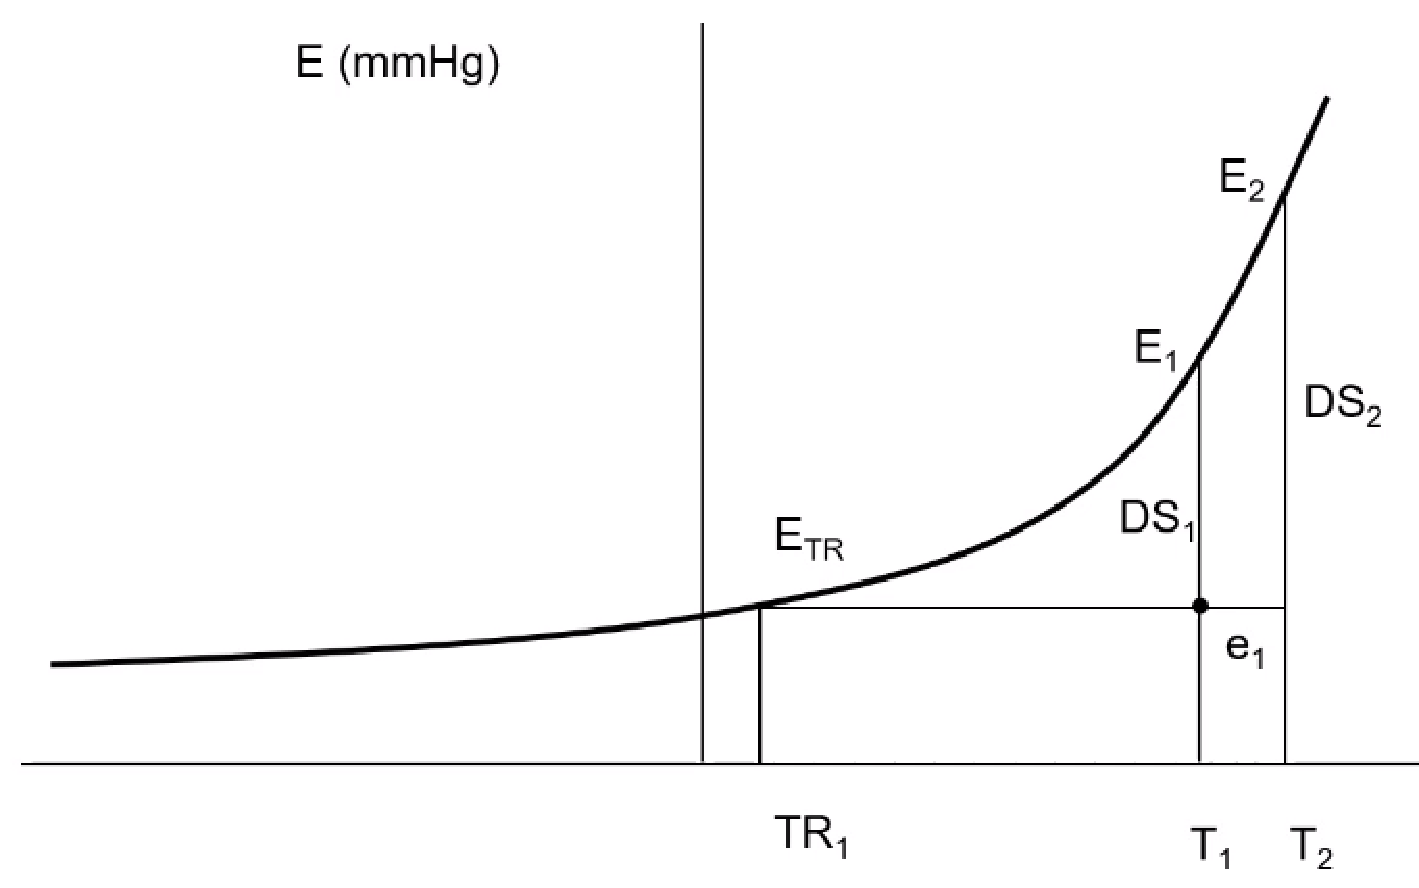
\includegraphics[width=0.5\textwidth]{ma7.pdf}
  \caption{Comportamiento del vapor de agua y la temperatura en la Evapotranspiración}
  \label{ma7}
\end{figure}\subsubsection{Presión de vapor de agua actual}
Presenta una variación diaria algo diferente entre localidades, estaciones, pero en una localidad en un día sino existen factores que la modifiquen su variación es mínima y se puede considerar constante.

Cuando es presión de \textbf{vapor de agua actual e variación estacional}, se observa que en verano es cuando se presenta mayor cantidad de vapor de agua y la menor en invierno, lo anterior se debe a que en verano se tienen las temperaturas más altas y se tienen las más bajas en invierno.

La Presión de vapor de agua actual (e), Latitudinalmente, disminuye del ecuador a los polos en términos generales, la causa radica en que con el aumento en latitud, disminuye la temperatura y en consecuencia la capacidad del área para almacenar vapor de agua.

Anualmente, la humedad relativa está definida por las variaciones de la temperatura y de la precipitación, la humedad relativa máxima se presenta en otoño y la mínima al principio de la primavera. Con respecto a la oscilación térmica presenta un comportamiento inverso.

\subsection{Humedad atmosférica}

\begin{table}[h!]
    \centering
    \begin{tabular}{@{}llll@{}}
    \toprule
    $e$ & $T$ max & $T$ min & $T$ \\ \midrule
    e1  & T max1  & T min 1 & T1  \\
    e2  & T max2  & T min1  & T2  \\
    e3  & T max3  & T min 2 & T3  \\
    e4  & T max4  & T min2  & T4  \\
    e5  & T max5  & T min 3 & T5  \\
    e6  & T max6  & T min3  & T6  \\
    e7  & T max7  & T min 4 & T7  \\
    e8  & T max8  & T min4  & T8  \\
    e9  & T max9  & T min 5 & T9  \\ \bottomrule
    \end{tabular}
    \caption{Conjunto de pares de valores}
    \label{tabma8}
\end{table}
Creando un modelo de dispersión (Sin unir los puntos)
\begin{equation}
    e =F\left(T_{\max }\right)\lor F(T)\lor F\left(T_{\min }\right)
\end{equation}
\begin{figure}[h!]
\centering
  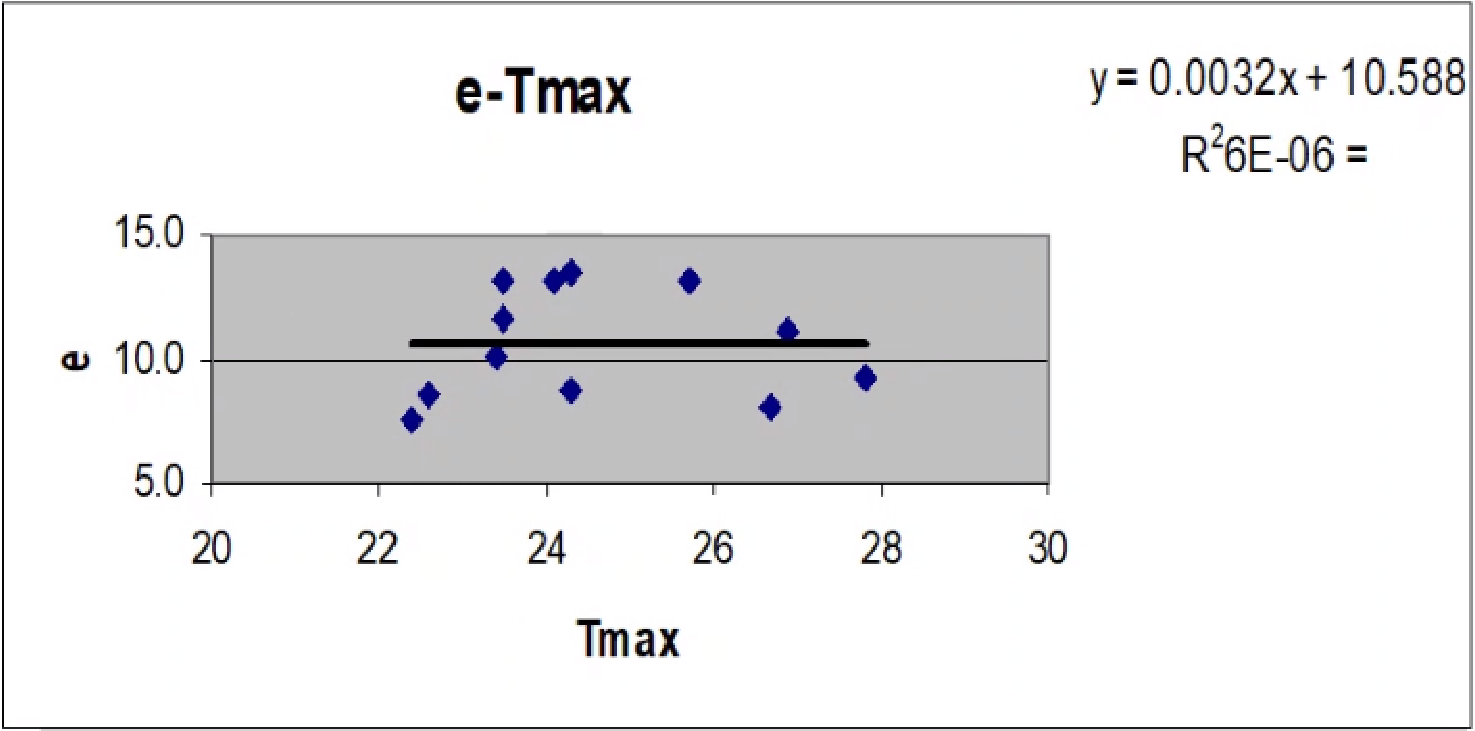
\includegraphics[width=0.5\textwidth]{ma8.pdf}
  \caption{Estimación de la presión de vapor de agua actual $e$}
  \label{ma8}
\end{figure}
\begin{figure}[h!]
\centering
  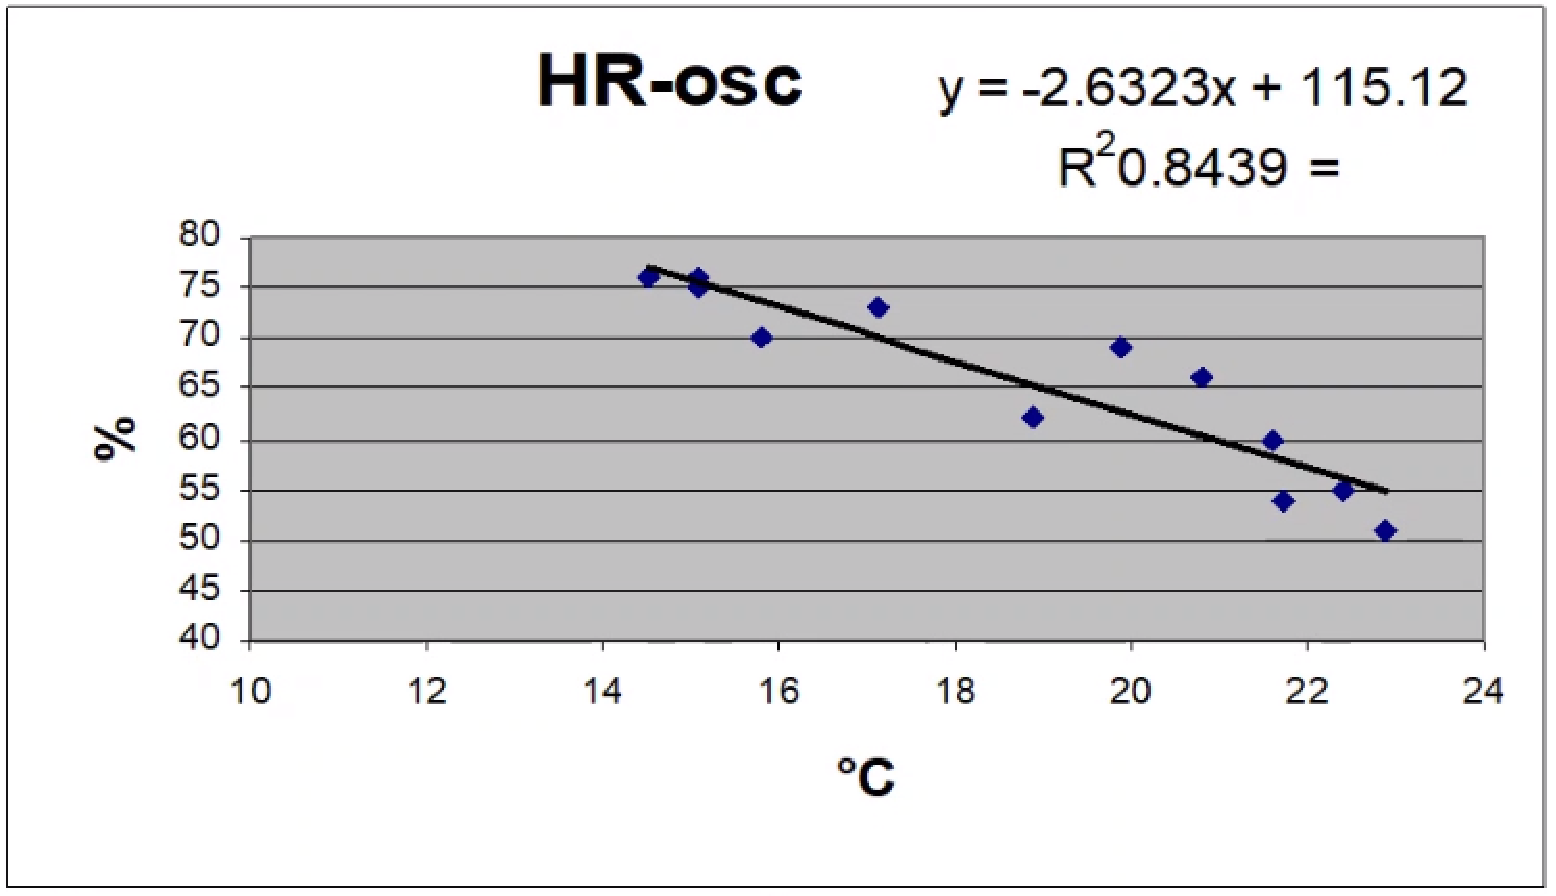
\includegraphics[width=0.5\textwidth]{ma9.pdf}
  \caption{Estimación de la humedad relativa}
  \label{ma9}
\end{figure}
\begin{figure}[h!]
\centering
  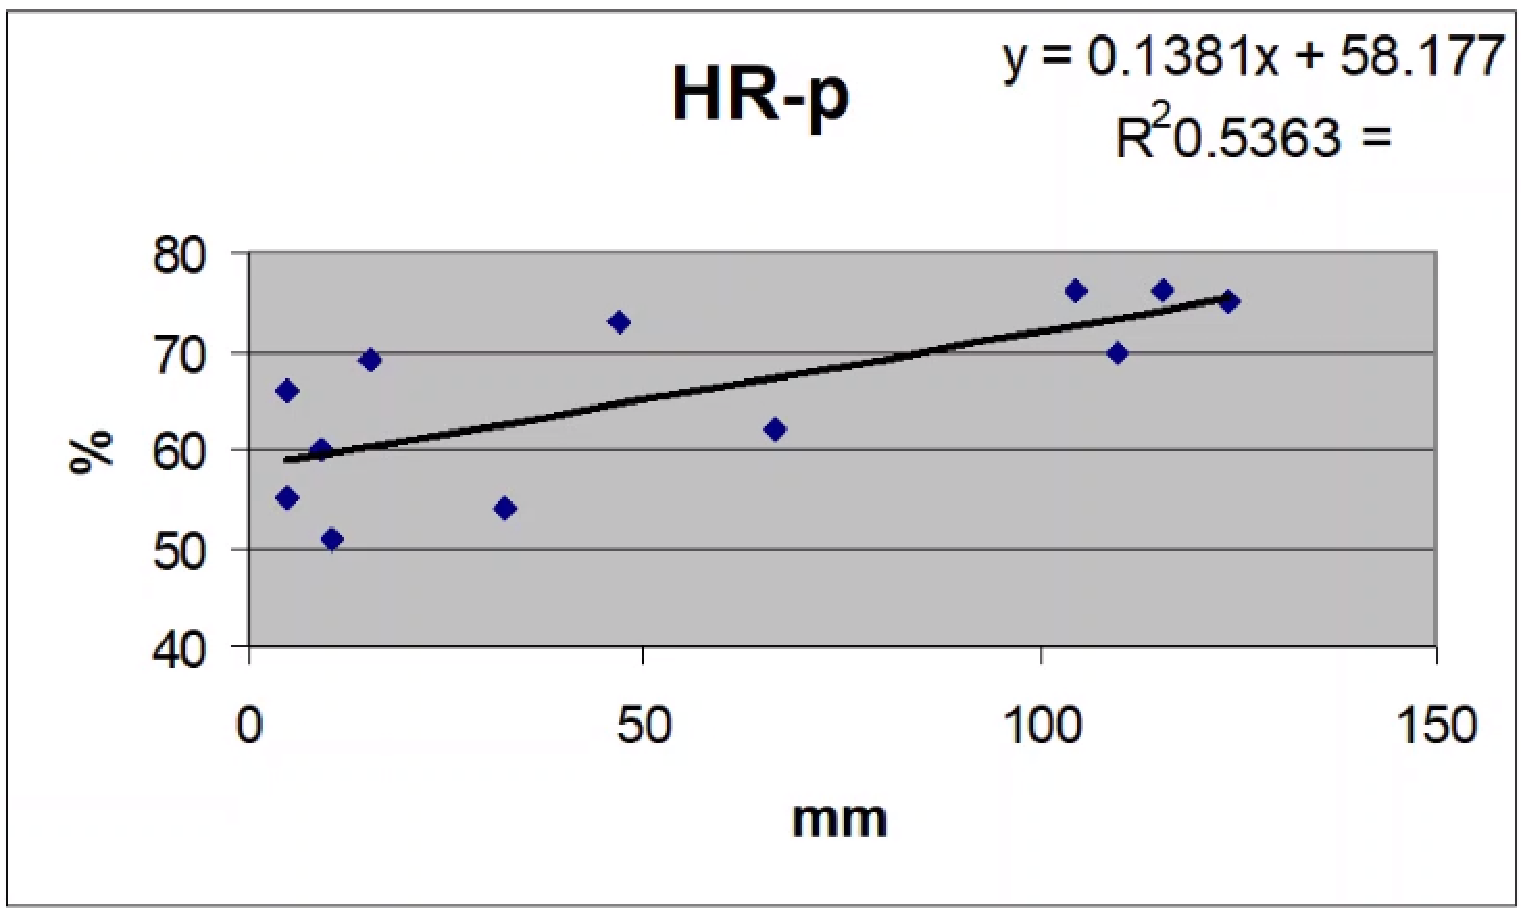
\includegraphics[width=0.5\textwidth]{ma10.pdf}
  \caption{Estimación de la humedad relativa}
  \label{ma10}
\end{figure}
La utilidad de la estimación de la temperatura del punto de rocío, es que cuando el valor de $e$ pasa a ser $E$ de la ecuación siguiente:
\begin{equation}
    E = 4.58 \times 10^{\frac{7.5T}{237.3T}}
\end{equation}
\subsection{Radiación}
\begin{definition}[Radiación térmica]
    Es una de las tres formas básicas de transmisión de energía. De los diferentes tipos de radiación se hará referencia a a la radiación térmica que es la radiación emitida por todos los cuerpos. Está ligada a la temperatura de los mismos.
\end{definition}
\begin{definition}[Flujo radiante]
    Es la cantidad de energía emitida por unidad de tiempo de un cuerpo:
    \begin{equation}
        F = \frac{E}{t}\left(\frac{joules}{segundos}\right) = watts
    \end{equation}
\end{definition}
\begin{definition}[Flujo radiante]
    Es la cantidad de energía emitida por unidad de tiempo (flujo radiante) y por unidad de superficie:
    \begin{equation}
        D = \frac{Flujo}{Area}
    \end{equation}
\end{definition}
\begin{definition}[Irradiancia]
    Es la cantidad de energía recibida por unidad de tiempo por unidad de área en una superficie
    \begin{equation}
        I=\frac{F}{Area} =\left(\frac{calorias}{minutos\cdot cm^2}\right)
    \end{equation}
\end{definition}
\begin{definition}[Irradiación]
    Energía incidente en una superficie por unidad de área, obtenida al integrar la irradiancia en un periodo de tiempo como un día:
\end{definition}
\begin{definition}[Cuerpo negro]
    La ausencia de reflexión es lo que da origen a su nombre, es un concepto teórico para designar el perfecto radiador y perfecto absorbedor; éste es un estándar con el cual pueden compararse las características de radiación de otros cuerpos. Es el que emite y absorbe a cualquier temperatura y en cualquier longitud de onda la máxima cantidad de radiación
\end{definition}
\begin{figure}[h!]
\centering
  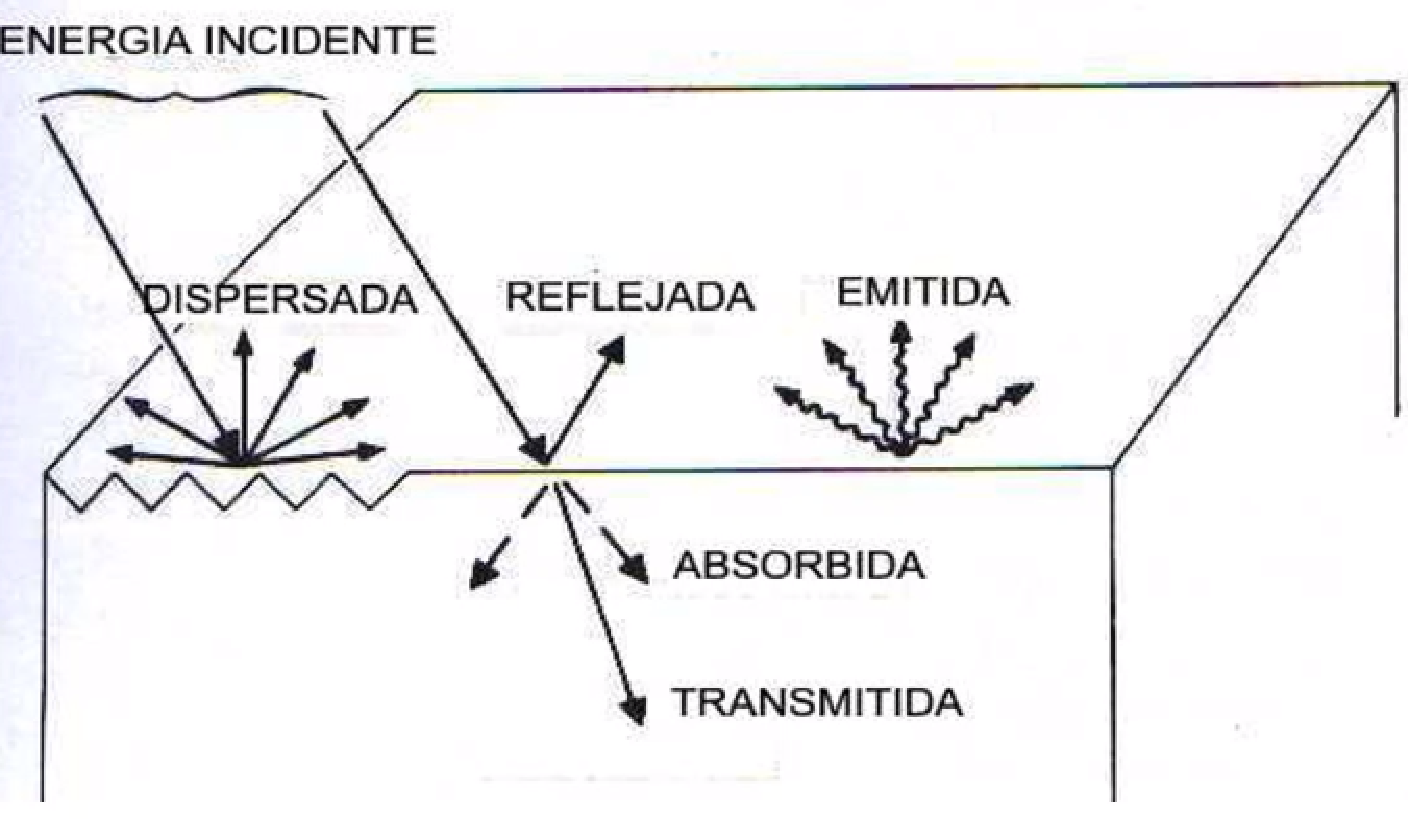
\includegraphics[width=0.5\textwidth]{ma11.pdf}
  \caption{Interacción de la radiación con la materia}
  \label{ma11}
\end{figure}
\begin{definition}[Emisividad $(\xi)$]
    Es la relación que existe entre la energía que emite un cuerpo ($E$) y la máxima energía que emite el cuerpo negro $(E_N)$ por ejemplo si $\epsilon_N=1$ y $\epsilon_b=0$ entonces $\epsilon\left(0,1\right)$:
    \begin{equation}
        \epsilon \frac{E}{E_N}
    \end{equation}
\end{definition}
\begin{definition}[Absorción ($a$)]
    Es la relación que existe entre la energía absorbida ($E_a$) por un cuerpo y la energía total ($E_T$) que incidió en éste:
    \begin{equation}
        a =\frac{E_a}{E_T}
    \end{equation}
\end{definition}

\begin{definition}[Reflexión (albedo $\alpha$)]
    Es la relación entre la energía reflejada ($E_a$) por un cuerpo total :
    \begin{equation}
        \alpha =\frac{E_a}{E_T}
    \end{equation}
\end{definition}
\begin{definition}[Transmisión ($t$)]
    Es la relación que existe entre la energía transmitida ($E_T$) por un cuerpo y la energía total ($E_T$) que incidió el cuerpo
    \begin{equation}
        t =\frac{E_t}{E_T}
    \end{equation}
\end{definition}
\begin{figure}[h!]
\centering
  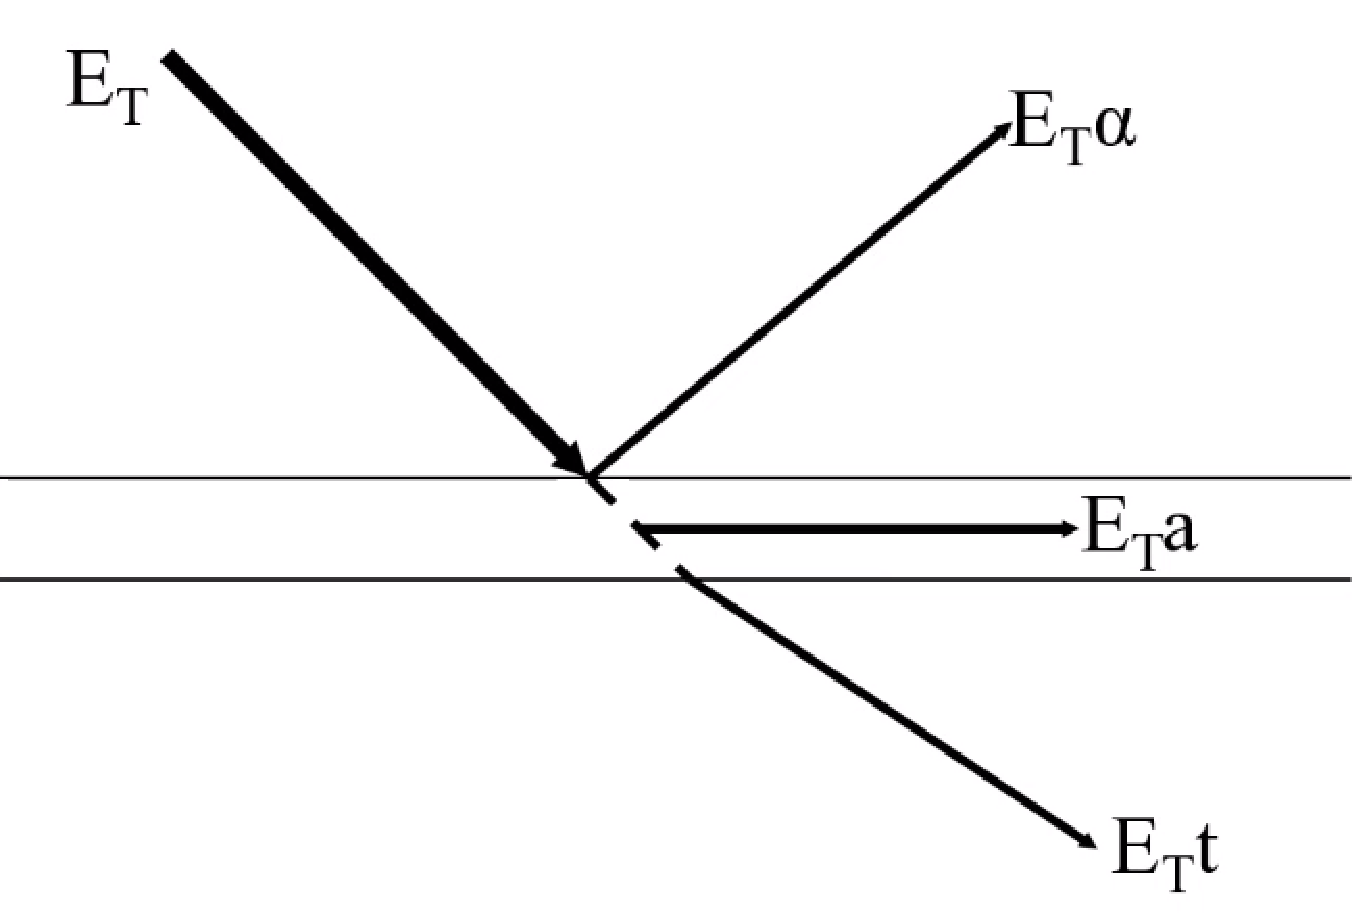
\includegraphics[width=0.5\textwidth]{ma12.pdf}
  \caption{Radiación incidente en un cuerpo transparente}
  \label{ma12}
\end{figure}
\begin{align}
    &E_T =E_T\alpha + E_Tt+ E_Ta\\
    &I = \alpha + t + a
\end{align}
\begin{figure}[h!]
\centering
  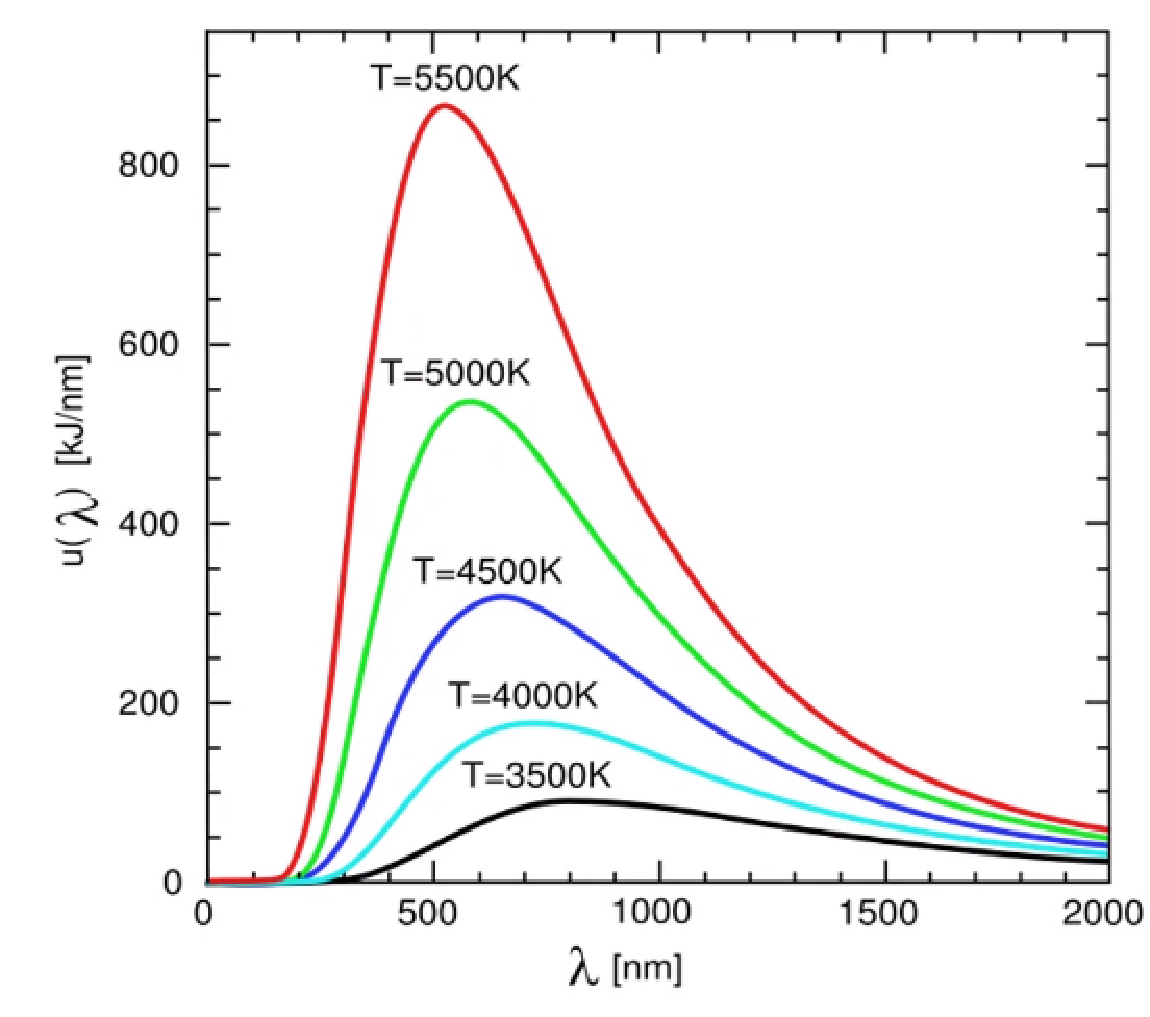
\includegraphics[width=0.5\textwidth]{ma13.pdf}
  \caption{Planck}
  \label{ma13}
\end{figure}
El espectro de emisión de energía emitida por un cuerpo en una función de su temperatura absoluta y de las longitudes de onda, de donde emite.
\begin{equation}
    D_{N,\lambda} f\left(T,\lambda\right)\implies D_{N,\lambda} = \frac{C_1}{\lambda^5\left(e^{\frac{C_2}{\lambda T}} - 1\right)}
\end{equation}
$D_{N,\lambda}$ Es la emisión de energía monocromática del cuerpo negro ($cal\cdot cm^{-2}\cdot min^{-1}\cdot \mu m^{-1}$), $C_1$ es $5.362\times 10^5$ en $(cal\cdot cm^{-2}\cdot min^{-1}\cdot \mu m^4)$, $C_2=1.4385\times 10^4$ en $(\mu\cdot m)$ Kelvin y por último $\lambda, \mu m$ es la longitud de onda que emite un cuerpo $T$ en Kelvin.
\begin{definition}[Stefan-Boltzmann]
    La cantidad total de energía emitida por un cuerpo negro en todas las longitudes de onda es directamente proporcional a su temperatura absoluta a la cuarta potencia
    \begin{equation}
        D_N \sigma T^4
    \end{equation}
    $D_N$ en ($cal\cdot cm^{-2}\cdot min^{-1}$), $T$ es la temperatura del cuerpo en $K$, $\sigma$ es la constante de Stefan-Boltzmann $\sigma=8.13\times 10^{-11}$ en ($Cal\cdot cm^{-2}\cdot min^{-1}\cdot K^-4$), para otros cuerpos se calcula con la siguiente relación $D=\epsilon\cdot \sigma T^4$, $\epsilon$ es el coeficiente de emisividad del cuerpo:
    \begin{equation}
        \epsilon = \frac{D}{\sigma\cdot T^4}= \frac{D}{D_N}
    \end{equation}
\end{definition}
\begin{figure}[h!]
\centering
  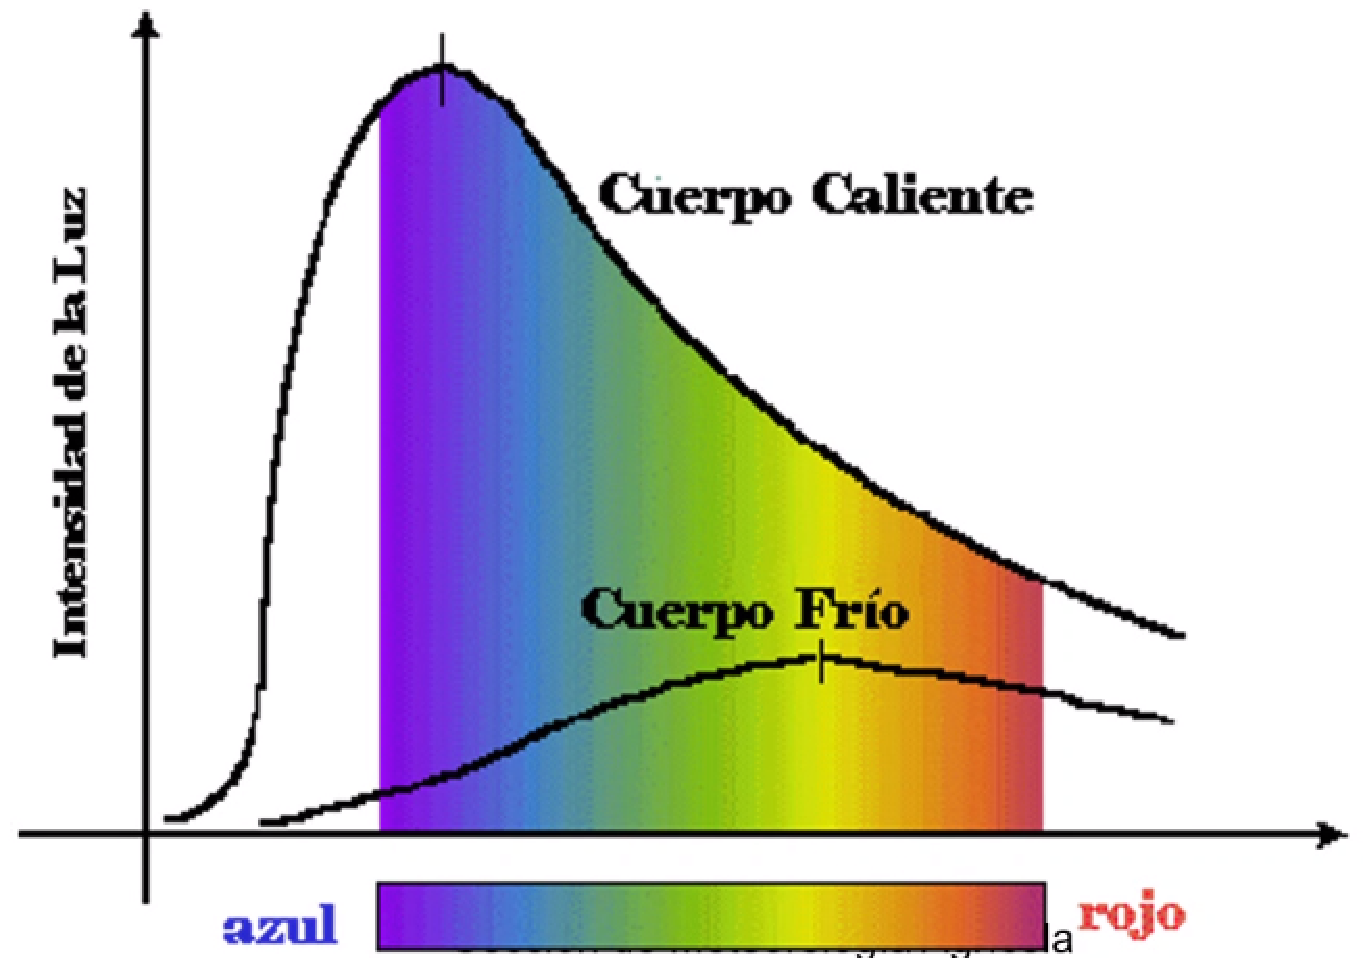
\includegraphics[width=0.5\textwidth]{ma14.pdf}
  \caption{Ley de Wien}   
  \label{ma14}
\end{figure}
\begin{definition}[Wien]
    La longitud de onda ($\lambda_{max}$) donde se representa la máxima emisión de energía de un cuerpo es inversamente proporcional a al temperatura absoluta de éste. Existe una razón inversamente proporcional entre la temperatura de un cuerpo negro y su longitud de onda donde se presenta la máxima emisión de energía:
    \begin{equation}
        \lambda_{\max }= \frac{C}{T}
    \end{equation}
\end{definition}
\begin{definition}[Kirchhoff]
    Un cuerpo que es buen emisor en una longitud de onda y a su temperatura también es buen absorbedor en esas condiciones; la capacidad de absorción de un cuerpo es igual al poder de emisión en una misma longitud de onda a la misma temperatura:
    \begin{equation}
        e_{\lambda} = a_{\lambda}
    \end{equation}
\end{definition}


\begin{example}
    Calcular $a$ y $b$:
    \begin{table}[h!]
        \centering
        \begin{tabular}{@{}ccc@{}}
        \toprule
        dj  & $IG (cal\cdot cm^{-2}\cdot min^{-1})$ & $n (h)$ \\ \midrule
        17  & 518                                   & 7.31    \\
        47  & 516                                   & 8.26    \\
        75  & 611                                   & 8.1     \\
        105 & 561                                   & 7.92    \\
        135 & 544                                   & 7.88    \\
        162 & 444                                   & 6.24    \\
        198 & 467                                   & 5.75    \\
        228 & 492                                   & 6.29    \\
        258 & 409                                   & 5.41    \\
        288 & 430                                   & 6.83    \\
        318 & 441                                   & 7.78    \\
        345 & 441                                   & 7.42    \\ \bottomrule
        \end{tabular}
        \caption{Latitud ($\phi) = 19.5\circ N$}
        \label{tabma9}
\end{table}
\end{example}
Procedimiento:
\begin{align*}
    &d = 23.45\sin{\left(\frac{360(284 +dj)}{365}\right)}\\
    &h_5 = \arccos{ -\tan{(\phi)}\tan{(d)}}\\
    &N =\frac{2h_5}{15}\\
    &I_0= 1.974\\
    &I_A=\frac{1440}{\pi}I_0\left(1 + 0.033\cos{\frac{360dj}{365}}\right)\left(0.01745h_5\sin{(\phi)}\sin{(d)} +\cos{(\phi)}\cos{(d)}\sin{(h_5)}\right)\\
\end{align*}

\begin{table}[h!]
    \centering
    \begin{tabular}{@{}ccc@{}}
    \toprule
    Fecha & Mes        & dJ  \\ \midrule
    17    & Enero      & 17  \\
    16    & Febrero    & 47  \\
    16    & Marzo      & 75  \\
    15    & Abril      & 105 \\
    15    & Mayo       & 135 \\
    11    & Junio      & 162 \\
    17    & Julio      & 198 \\
    16    & Agosto     & 228 \\
    15    & Septiembre & 258 \\
    15    & Octubre    & 288 \\
    14    & Noviembre  & 318 \\
    11    & Diciembre  & 345 \\ \bottomrule
    \end{tabular}
    \caption{Días recomendados de cada mes}
    \label{tabma10}
\end{table}
Se realiza el diagrama de dispersión entre $Ig/IA$ y $n/N$ y se determina su modelo lineal.

Con el método gráfico, cálculo de $a$ y $b$ de forma gráfica, para este método se necesita conocer el promedio anual de $n/N$, y con este valor se entra a la figura \ref{ma15} y se calculan los valores de a y b. 
\begin{figure}[h!]
\centering
  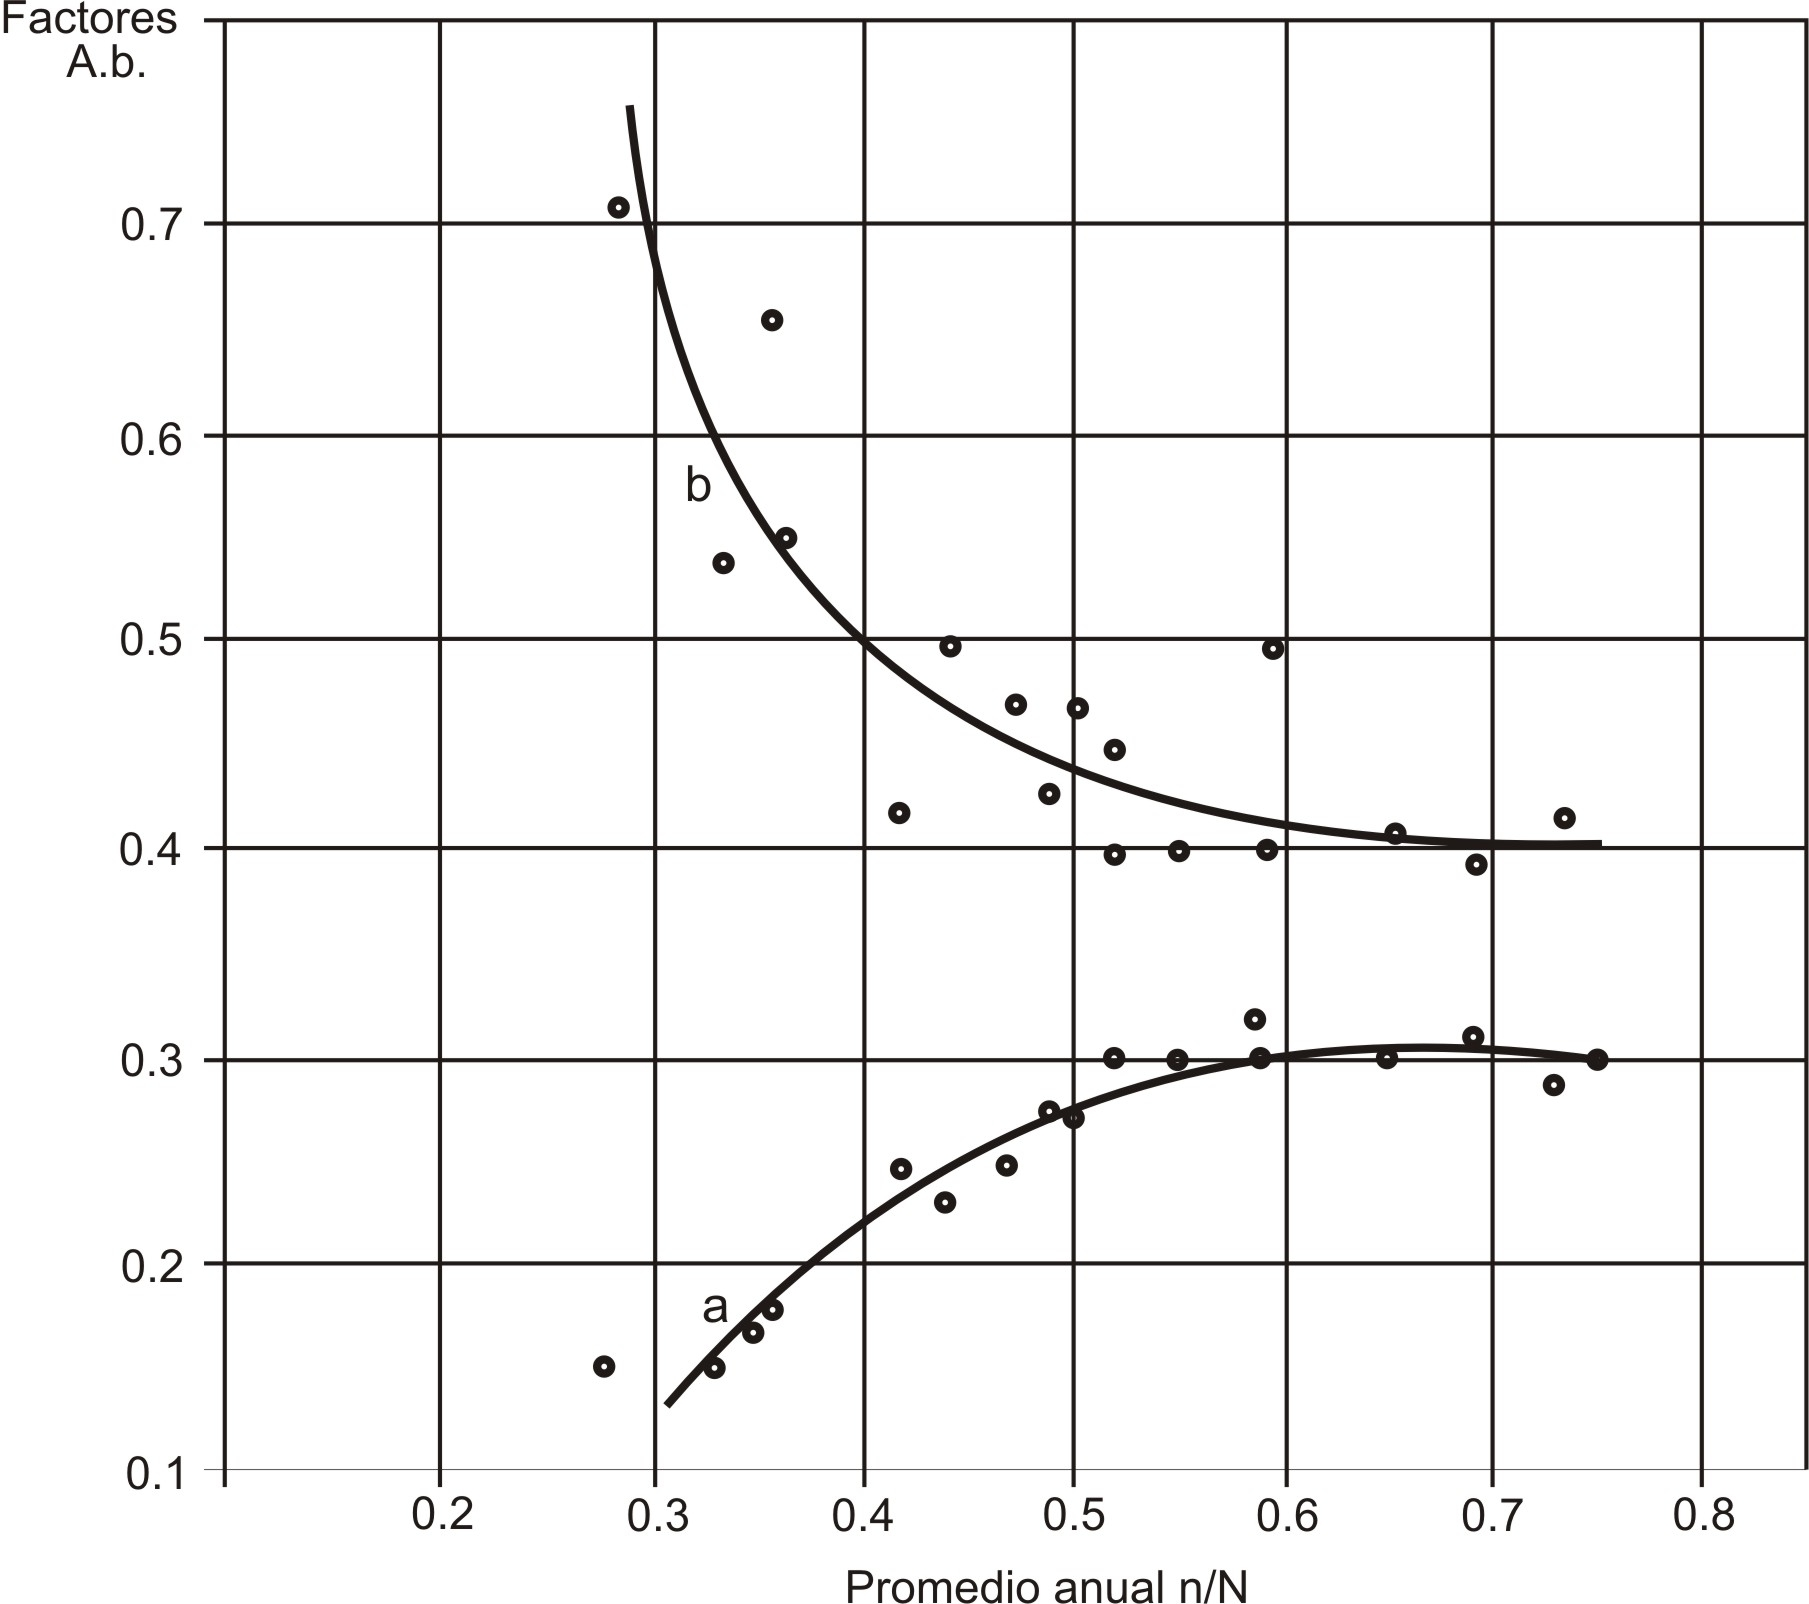
\includegraphics[width=0.5\textwidth]{ma15.png}
  \caption{Gráfica para determinar los valores de a y b de la expresión de Prescott.}
  \label{ma15}
\end{figure}
Con cada ecuación, estime los valores de Ig para cada mes e indique cual método es mejor.

\section{Radiación}

¿Cómo varía el ángulo cenital?
\begin{itemize}
    \item $Z$, varía con la época del año (d, declinación solar), la latitud ($\phi$) y la hora del día (ángulo horario del sol, $h$)
    \item $Z$ no se mide por lo general directamente sino que se determina con la siguiente relación:
    \begin{equation}
        \cos{Z} = sen{\phi} \cdot \sen{d}+ \cos{\phi} \cdot \cos{d} \cdot \cos{h}
    \end{equation}
\end{itemize}

Para calcular el Ángulo Horario de la salida del Sol:
\begin{itemize}
    \item Se debe conocer la Velocidad a la que gira la Tierra: $v=\frac{360^{\circ}}{24hrs}=15^{\circ}/h$
    \item El ángulo horario se forma entre el meridiano del lugar y el círculo horario meridiano del lugar que pasa por dicho astro y se calcula con las siguientes relaciones:
    \begin{align*}
        &h=15\left(12- x\right)&&x < 12\\
        &h=15\left(x -12\right)&&x > 12
    \end{align*}
    Donde x es la hora del día.
    \item En los equinoccios la $d = 0^{\circ}$ y al medio día solar, $h = 0^{\circ}$ 
    \begin{align}
        &\cos{z} = \sen{\phi} \cdot \sen{d} + \cos{\phi} \cdot \cos{d} \cos{h}\\
        &\cos{Z}= \sen{\phi} \cdot \sin{ 0^{\circ}} + \cos{\phi} \cos{0^{\circ}} \cdot \cos0^{\circ}\\
        &\cos{Z} = Cos{\phi}
    \end{align}
    Sí a ambos términos se les obtiene el arcos. $Z=\phi$
    \item Al medio día solar $h=0^{\circ}$ \begin{equation}
        \cos{Z}= \sen{(\phi)} \cdot \sen{(d)} + \cos{(\phi)} \cdot \cos{(d)}
    \end{equation}
    Finalmente $Z=\phi-d$
    \item El ángulo horario de la salida del sol (hs); al momento se pone el ángulo $Z= 90^{\circ}$.
    \begin{align}
        & \cos{90^{\circ}} = \sin{\phi} \cdot \sin{d} + \cos{\phi} \cdot \cos{d} \cdot \cos{h_s}\\
        & 0 = \sin{\phi} \cdot \sin{d} + \cos{\phi} \cdot \cos{d} \cdot \cos{h_s}\\
        & h_s = \arccos{ -\tan{\phi} \cdot \tan{d}} 
    \end{align}
    \item La hora en que astronómicamente sale el sol se determina con la siguiente relación:
    \begin{equation}
        X_s = 12 - \left(\frac{h_s}{15}\right)
    \end{equation}
    \item Como se observa en la relación para obtener $h$, es cero al medio día y aumenta $15^{\circ}$ por hora antes y después, así para obtener el número de horas al medio día solar únicamente se tiene que dividir entre $15^{\circ}$ el valor de $h_s$. La expresión para el cálculo de la duración astronómica del día o fotoperiodo (N) es:    
    \begin{align}
        &N = \frac{2h_s}{15}\\
        &d = 0^{\circ}\\
        &h_s = \arccos{ -\tan{19.5^{\circ}} \tan{0^{\circ}}}\\
        &h_s = 90^{\circ}\\
        &N = \frac{2 \cdot 90^{\circ}}{15h^{ - 1}} = 12 h 
    \end{align}
    $\phi = 0^{\circ}$, en el ecuador la duración del día es 12 horas.
\end{itemize}
Si la radiación es cuasiparalela (rayos solares)

\subsubsection{Irradiación solar total diaria en una superficie horizontal ignorando la atmósfera}

Sí se quiere conocer conocer la cantidad cantidad de radiación radiación solar recibida en un intervalo, se determina integrando $I_h$ de la siguiente forma: 
\begin{equation}
    \int_{ -t}^t I_h\, dt = \int_{ - t}^t I \cdot \cos{Z}\, dt 
\end{equation}
Sí se quiere calcular la cantidad total de radiación solar en un día se utiliza la siguiente expresión:
\begin{equation}
    I_A = \frac{1440}{\pi}\left[\left(I_o\right) \cdot\left(1 +0.033\cos{\frac{360dj}{365}}  \right) \right]\cdot \left[0.01745(h_s) \cdot \sin{\phi} \cdot \sin{d} + \cos{\phi} \cdot \cos{d} \cdot \sin{h_S} \right]
\end{equation}
\begin{figure}[h!]
\centering
  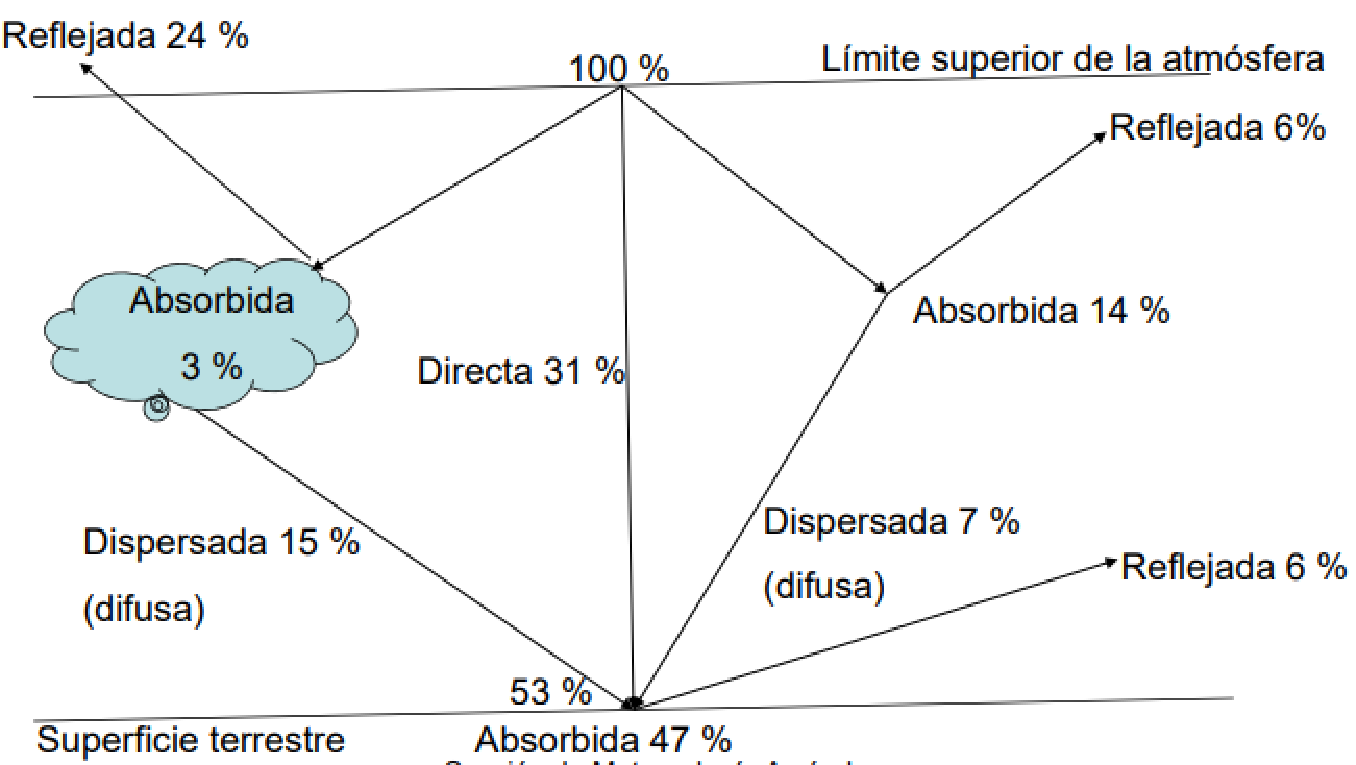
\includegraphics[width=0.5\textwidth]{ma16.pdf}
  \caption{Alteración típica cualitativa de la radiación solar a su paso por la atmósfera terrestre solar a su paso por la atmósfera terrestre día medio nublado}
  \label{ma16}
\end{figure}
La reducción de la radiación solar en términos generales
\begin{itemize}
    \item En un día medio nublado
    \item En un día totalmente despejado En un día totalmente despejado
    \item En un día totalmente nublado
\end{itemize}
\begin{table}[h!]
    \centering
    \begin{tabular}{ll}
    Gas           & Zona de absorción $(\mu m)$ \\
    Oxígeno       & 0.12-0.18                   \\
    Ozono         & 0.2-0.33                    \\
    Ozono         & 0.44-0.76 (parcialmente)    \\
    Vapor de agua & 0.93,1.13,1.42 y 1.47       \\
    $CO_2$        & 2.7                        
    \end{tabular}
    \caption{Gases que absorben la radiación solar}
    \label{tabma11}
\end{table}
Se puede concluir que la disminución y alteración alteración de la radiación radiación solar a su paso por la atmósfera se debe:
\begin{itemize}
    \item A la acción absorbente de los gases atmosféricos
    \item A la dispersión provocada por moléculas de aire y partículas sólidas en sus pensión
    \item A la reflexión de los rayos solares por las nubes
    \item La atmósfera se comporta como un cuerpo transparente con respecto respecto a la radiación solar.
\end{itemize}
Se tiene que una parte de la radiación solar es transmitida por la atmósfera y llega en forma directa a la superficie terrestre a la superficie terrestre

Mientras que otra parte presenta los fenómenos de dispersión y reflexión que producen una de dispersión y reflexión que producen una desviación de los rayos solares generando la radiación solar radiación solar difusa (dispersa) (dispersa)

La suma de la radiación solar directa y la difusa en una superficie horizontal se denomina en una superficie horizontal se denomina radiación solar global o total y sus unidades son $cal\cdot cm^{-2}\cdot  dia^{-1}$

\subsubsection{Espectro de emisión del sol Espectro de emisión del sol}
El sol se considera como un cuerpo negro
con una temperatura de $6000^{\circ}K$. Al aplicar la ley de Planck se conoce la distribución espectral o composición de longitud de onda y su emisión
monocromática. El espectro de emisión del sol está en el siguiente rango:
\begin{equation}
    0.3 <\lambda_s\leq 3\mu m
\end{equation}
\begin{definition}[Radiación ultravioleta]
    También es conocida como química, está formada por radiaciones cuya longitud de onda es muy corta $< 0.4 \mu m$
\end{definition}
\begin{definition}[Radiación luminosa]
    Es la luz visible, su longitud se encuentra entre las 0.4 y las $0.7 \mu m$.
\end{definition}
\begin{definition}[Radiación infrarroja]
    Es conocida conocida como térmica; son las ondas que presentan una longitud $> 0.7 \mu m$.
\end{definition}
La energía total emitida por el sol, se obtiene con la ley de Stefan-Boltzman:
\begin{align}
    &D_s = \sigma T^4\\
    &\sigma = 8.13\cdot 10^{ - 11}\\
    &D_s = 8.13\cdot 10^{ -11}\cdot 6000^4\\
    &D_s 105364.8\, cal\cdot cm^{ - 2}\cdot \min^{ - 1}
\end{align}
El área esférica del sol ($A_s$) es $5.28\times 10^{22}\cdot cm^{ - 2}$
\begin{align}
    &F_s = D_s\cdot A_s\\
    &F_s = 105364.8\cdot 5.28\times 10^{22}\\
    &F_s = 5.56\times 10^{26}\, cal\cdot cm^{ - 2}
\end{align}
Ésta se determina con la ley de Wien
\begin{equation}
    \lambda_{\max} = \frac{2897}{6000} = 0.483\mu m
\end{equation}
La longitud de onda donde se presenta la máxima emisión de sol está comprendida dentro del espectro visible del sol.
\begin{itemize}
    \item Espectro ultravioleta $\lambda \leq 0.4\mu m$
    \item Espectro visible $0.4 < \lambda \leq 0.78\mu m$
    \item Espectro infrarrojo $\lambda > 0.78\mu m$
\end{itemize}
La longitud de onda donde emite el sol se le denomina longitud de onda corta.
\begin{definition}[Radiación solar extraterrestre]
    Es la energía solar que se recibe en un cuerpo o plano que está en el limite superior de la atmósfera.
Constante sola $(I_0)$. Es la cantidad de energía del sol que se recibe (Irradiancia) en un plano perpendicular a los rayos solares, el cual está en el límite su perio r de la atmósfera y cuando se tiene la distancia media entre la tierra y el sol.
\begin{equation}
    I_0 = \frac{F}{4 \pi \bar{d}^2}
\end{equation}
Donde $\bar{d}^2$ es la distancia media entre la tierra y el sol ($149.7\times 10^{11}$) e $I_0=1.974 cal \cdot cm^{-2}\cdot min^{-1}$
\end{definition}

En realidad el valor de la constante solar presenta variaciones debido a la órbita de la tierra alrededor del sol, por lo que cuando su distancia real sea ``d'' el valor relativo (real) de la constante Solar ``$I$'' en el exterior de la atmósfera se obtiene con la siguiente relación en cal $cm^{-2}$ $min^{-1}$:
\begin{align}
    &I = \left(\frac{\bar{d}^2}{d}\right)\cdot I_0\\
    &I = I_0\left(1 +0.033 \cos{\left(\frac{360dj}{365}\right)}  \right)
\end{align}
\begin{figure}[h!]
\centering
  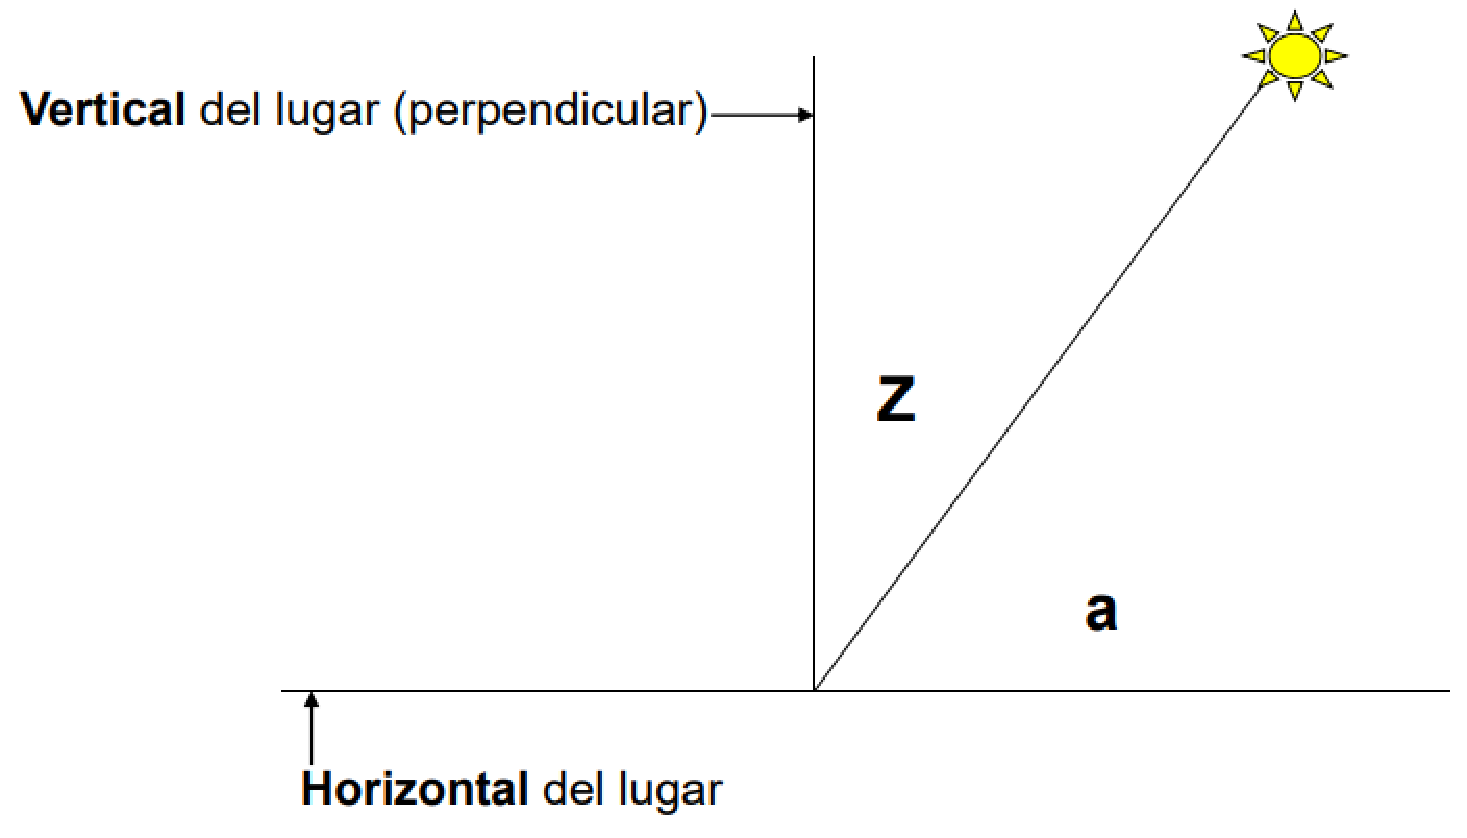
\includegraphics[width=0.5\textwidth]{ma17.pdf}
  \caption{Ángulo Zenital (Z) y ángulo de Elevación solar (a)}
  \label{ma17}
\end{figure}
\begin{figure}[h!]
\centering
  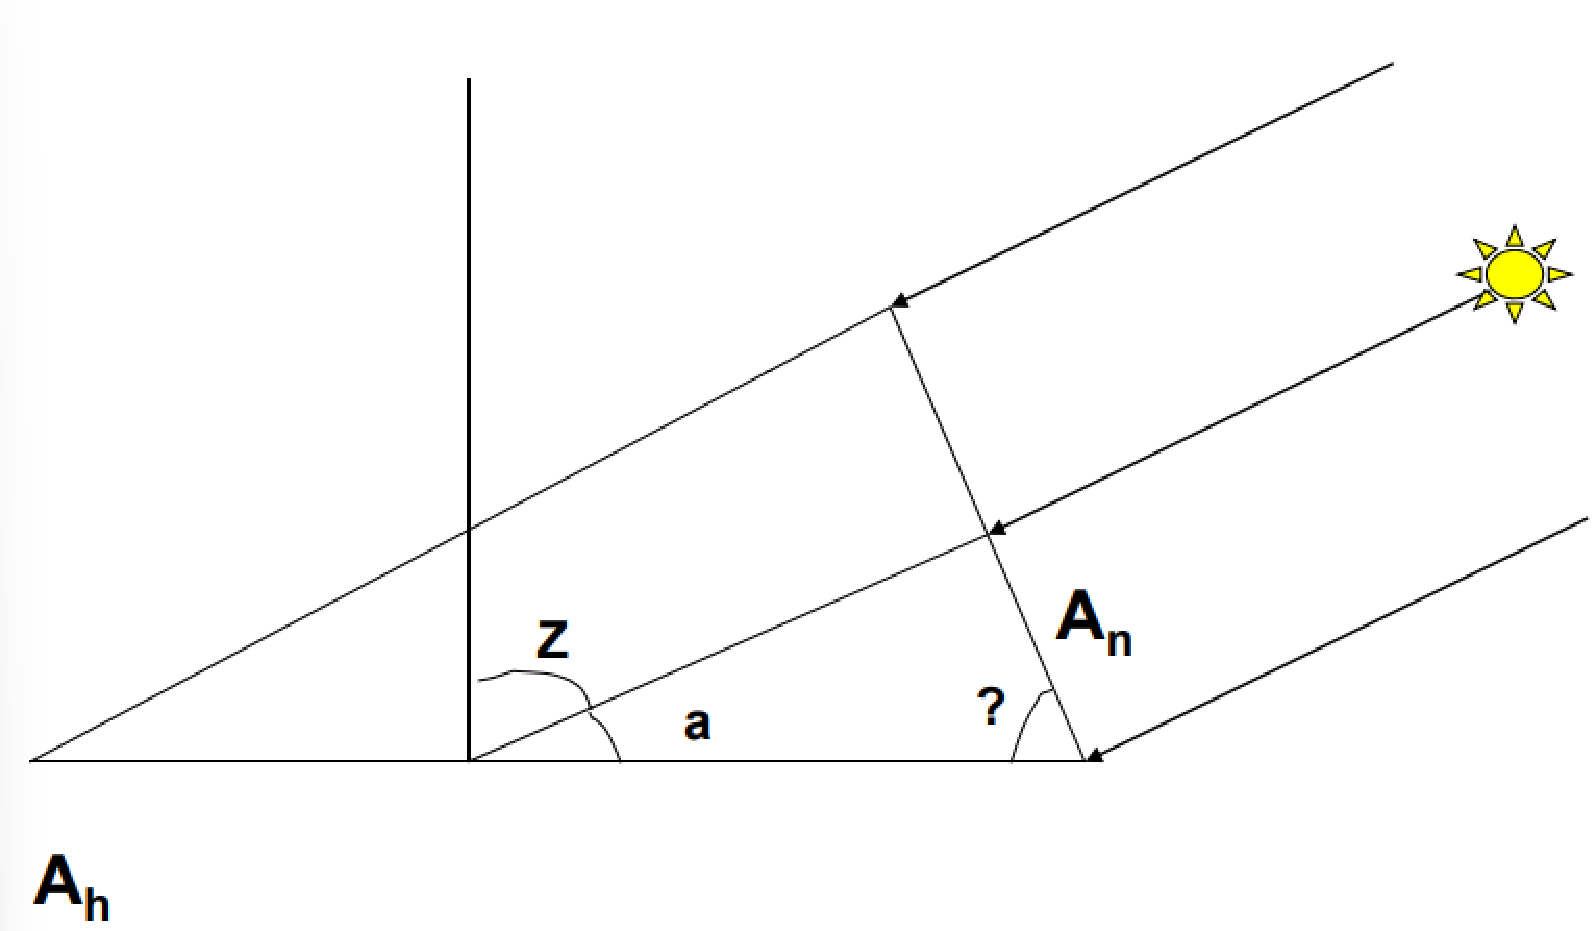
\includegraphics[width=0.5\textwidth]{ma18.pdf}
  \caption{Radiación solar recibida (irradiancia) en una superficie horizontal ($I_h$) en el exterior de la en el exterior de la atmósfera}
  \label{ma18}
\end{figure}
La relación que existe entre ambas superficies está dada por:
\begin{equation}
    \cos{(Z)} = \frac{A_n}{A_h} 
\end{equation}
Como las superficies $An$ y $Ah$ están en el tope de la atmósfera atmósfera y dado que ahí no hay medios absorbentes de la radiación solar, entonces la cantidad de energía (E) que pasa a través de ambas superficies debe ser la misma y se tiene que:
\begin{equation}
    EA_n = A_h
\end{equation}
El valor de $I_h$ también se expresa en función del ángulo de elevación solar ``$a$'' con la siguiente relación y en las mismas unidades:
\begin{equation}
    I_h = I_0\left(1 +0.033 \cos{\left(\frac{360dj}{365}\right)}\right)\cdot \sin{(a)} 
\end{equation}
Pero en términos de Z:
\begin{equation}
    I_h = I_0\left(1 +0.033 \cos{\left(\frac{360dj}{365}\right)}\right)\cdot \cos{(Z)} 
\end{equation}
\subsection{Estimación de la radiación solar global (total)}
Angstrom (1924) propone la siguiente expresión:
\begin{equation}
    I_G = I_D\left(a + b \cdot \frac{n}{N} \right)
\end{equation}
\begin{notation}
\begin{itemize}
    \item $I_G$: Radiación global en $cal$ $cm^{-2}$ $dia^{-1}$
    \item $I_D$: radiación solar de un día totalmente despejado
    \item $n$ horas brillo sol (duración de la insolación),
    \item $N$ Duración astronómica del día (Fotoperiodo),
    \item $a$ y $b$ son valores obtenidos por medio de regresión lineal simple.
\end{itemize}
\end{notation}
Prescott (1950) modifica la relación de Angstrom y propone la siguiente expresión:
\begin{equation}
    I_G = I_A\left(a + b \cdot \frac{n}{N} \right)
\end{equation}
\begin{notation}
$I_A$: Es el valor de Angot, $cal$ $cm^{-2}$ $dia^{-1}$
\end{notation}
Las dos constantes constantes (a y b) en teoría, están relacionadas relacionadas con los niveles de radiación difusa y con la atenuación de la radiación directa
En un día totalmente despejado:
\begin{align*}
    &\frac{n}{N} =1&& \frac{I_G}{I_A} = a + b
\end{align*}
a + b son el valor del coeficiente de transmisión de la atmósfera.

En un día totalmente nublado:
\begin{align*}
    &\frac{n}{N} =0&& \frac{I_G}{I_A} =a
\end{align*}

\begin{notation}
\begin{itemize}
    \item $a$, es el coeficiente de transmisión de las nubes. Está relacionado con la radiación solar (difusa)
    \item $b$, esta relaciona da con la radiació n directa (solar).
\end{itemize}
\end{notation}
\subsubsection{Estimación de los coeficientes a y b de la ecuación de Prescott}
Por \textbf{regresión Lineal}: en este caso se deben tener datos medidos de $IG$ y de $n$, y se procede de la siguiente manera:
\begin{align*}
    &I_G = I_A\left(a + b \cdot \frac{n}{N} \right)\\
    &\frac{I_G}{I_A} = a + b\cdot \frac{n}{N}\\
    &\frac{I_G}{I_A} = Y\quad X = \frac{n}{N}
\end{align*}
Por lo que $Y = a + bX$.

La otra forma de estimación, es \textbf{Gráficamente} por Frere (1974) que propone la figura \ref{ma19}:
\begin{figure}[h!]
\centering
  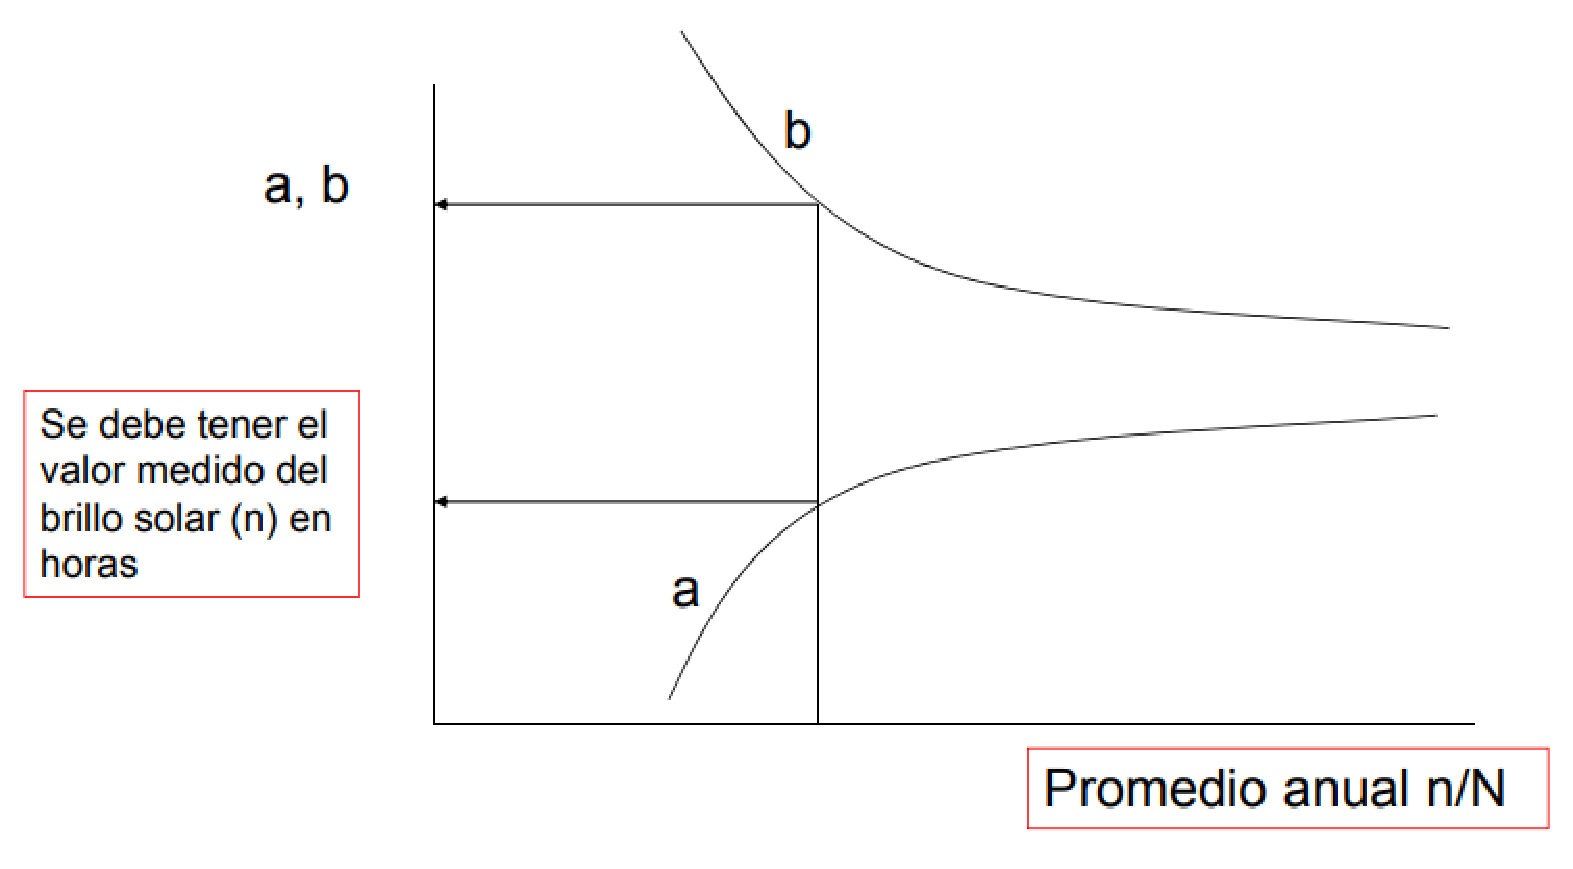
\includegraphics[width=0.5\textwidth]{ma19.pdf}
  \caption{Gráfica de Frere (1974)}
  \label{ma19}
\end{figure}
\begin{table}[h!]
    \centering
    \begin{tabular}{@{}lll@{}}
        \toprule
        \multicolumn{3}{l}{Por zona climática} \\ \midrule
        Clima              & a       & b       \\
        Fría y templada    & 0.18    & 0.55    \\
        Tropical seca      & 0.25    & 0.45    \\
        Tropical húmeda    & 0.29    & 0.42    \\ \bottomrule
        \end{tabular}
    \caption{Estimación de los coeficientes a y b de la ecuación de Prescott}
    \label{tabma12}
\end{table}
Norero propone la siguiente expresión (1970) para estimar $IG$
\begin{equation}
    I_G = I_A\left[\left(0.5 + 0.3 \cos{(\phi)}\right)  \cdot 0.5A^{0.09}\cdot \left(t +(1 - t)\cdot \frac{n}{N}\right) \right]
\end{equation}
\begin{notation}
    \begin{itemize}
        \item $I_G$ en $cal$ $cm^{-2}$ $dia^{-1}$
        \item $A$: altitud del lugar en m, sí $A\leq 360 m$, entonces: $0.59A^{0.09}=1$
        \item $t$: coeficiente de transmisión de las nubes
    \end{itemize}
\end{notation}
\begin{table}[h!]
    \centering
    \begin{tabular}{@{}cc@{}}
    \toprule
    Tipo de nube            & t    \\ \midrule
    Cirros                  & 0.83 \\
    Cirros estratos         & 0.75 \\
    Alto cúmulos            & 0.5  \\
    Alto estratos           & 0.4  \\
    Estrato cúmulos         & 0.33 \\
    Estrato                 & 0.25 \\
    Nimbo estrato           & 0.2  \\
    Cúmulos y cúmulos nimbo & 0.2  \\
    Niebla                  & 0.18 \\ \bottomrule
    \end{tabular}
    \caption{Coeficientes de transmisión (t) de diferentes nubes}
    \label{tabma13}
\end{table}
\subsubsection{Estimación de $I_G$ con datos de nubosidad}
La nubosidad se mide en octas o en décimos

En México el grado de nubosidad se mide y se
reporta con las siguientes tres categorías: \textbf{IG}, \textbf{medio nublado} y \textbf{nublado cerrado}

Para poder utilizar estas categorías es necesario transfórmalas a octas o décimos con la siguiente codificación:

\textbf{Octas}: día despejado (NDD) = 1, día medio nublado (NDMN)=4 día nublado(NDMN) = 4 y día nublado cerrado (NDNC) = 7

En \textbf{décimos}: Día despejado (NDD) = 1, día medio nublado (NDMN) = 5 y día nublado cerrado (NDNC) = 9
\begin{align}
    C_0 =\frac{N_D(1) + NDMN(4) + NDNC(7)}{\text{Número de días totales del mes}}
\end{align}

Black (1975) propone la siguiente relación:

Que necesita datos medidos de nubosidad
\begin{equation}
    I_G = I_A\left[0.803 - 0.304C - 0.458C^2\right]
\end{equation}
C, es la nubosidad media mensual en decimos y expresada en decimal NDD = 18, y C NDMN = 11 y NDNC = 2
$I_A=850$ $cal$ $cm^{-2}$ $dia^{-1}$
\begin{table}[h!]
    \centering
    \begin{tabular}{@{}cccccccccccc@{}}
    \toprule
    Oct           & 0    & 1    & 2    & 3    & 4    & 5    & 6   & 7    & 8   &      &    \\ \midrule
    $\frac{n}{N}$ & 0.95 & 0.85 & 0.75 & 0.65 & 0.55 & 0.45 & 0.3 & 0.15 &     &      &    \\
    Déc           & 0    & 1    & 2    & 3    & 4    & 5    & 6   & 7    & 8   & 9    & 10 \\
    $\frac{n}{N}$ & 0.95 & 0.85 & 0.8  & 0.75 & 0.65 & 0.55 & 0.5 & 0.4  & 0.3 & 0.15 &    \\ \bottomrule
    \end{tabular}
    \caption{Dorenbos y Pruitt (1974) proponen las siguientes relaciones entre $n/N$ y la nubosidad}
    \label{tabma14}
\end{table}

\subsubsection{Instrumentos para la medición de la radiación}

\begin{itemize}
    \item \textbf{Pirheliometros}: miden la radiación que llega perpendicularmente a una superficie
    \item \textbf{Piranómetros}: miden la radiación solar global
    \item \textbf{Solarímetrosy albedómetros}: uno mide la radiación global y el otro la radiación reflejada
    \item \textbf{Heliógrafos}: miden las horas brillo
    \item \textbf{Radiógrafos}: estiman la intensidad calorífica de la radiación solar
    \item \textbf{Pirgeómetro}: miden la radiación in frarroja emitida por la tierra
\end{itemize}

\subsection{Radiación solar}

\begin{definition}[Radiación Solar]
Es la energía que emite el sol en función de su temperatura absoluta.
\end{definition}
Su importancia radica en la  Fotosíntesis, Ciclo hidrológico Ciclo hidrológico; Es la fuente de energía de todos los procesos físicos y químicos que se presentan en la físicos y químicos que se presentan en la atmósfera y superficie terrestre.
\begin{definition}[La eclíptica]
    Círculo máximo de la esfera celeste, que forma con el ecuador un ángulo de $23^{\circ} 27'$ y señala el curso aparente del Sol durante el año
\end{definition}
\begin{figure}[h!]
\centering
  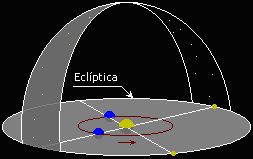
\includegraphics[width=0.5\textwidth]{ma20.png}
  \caption{La órbita de la Tierra alrededor del Sol define el plano que contiene a la eclíptica y, por tanto, el del movimiento aparente del Sol visto desde la Tierra.}
  \label{ma20}
\end{figure}
Determina las diferentes zonas térmicas de la
Tierra.

Regula la distribución de los cultivos

\subsubsection{Declinación solar (d)}
Es el ángulo que forman los rayos del sol con el plano del ecuador al medio día solar.

En otras palabra la declinación solar es un índice de alejamiento que
experimenta el Sol hacia el norte o hacia el sur
del ecuador. Ésta depende del día del año y es independiente de la latitud o de la localización del observador

Se determina con la siguiente Expresión (Cooper, 1969):
\begin{equation}
    d = 23.45 \sin{\left(\frac{360(284 +dj)}{365}\right)} 
\end{equation}
$d$ está en grados; variación de ``d'': d=0, d=+$23^{\circ} 27'$, $d=-23^{\circ} 27'$ y dj es el día juliano: primero de enero=1 31 de diciembre 365.

\subsubsection{Radiación terrestre}
Según la ley de Stefan-Boltzmann cualquier cuerpo cuya temperatura sea mayor al cero absoluto, emite energía y depende de la temperatura temperatura de éste.

La radiación terrestre es la energía que
emite la Tierra en su conjunto, en función
de su temperatura absoluta.


Sí se considera que la temperatura de la Tierra en su conjunto es casi constante e igual a 288 K ($15^{\circ}C$) su espectro de emisión se obtiene con la ley de Planck, con lo cual se determina en que longitud de onda emite ésta.

La longitud de onda en la cual emite la Tierra está comprendida entre los 4 a 60 Tierra está comprendida entre los 4 a 60$\mu m$.

La energía total que emite la Tierra en todas sus longitudes de onda se determina con la ley de Stefan-Boltzmann y su coeficiente de emisión ($\epsilon$) es 0.9
\begin{align}
    &D_T = \epsilon \sigma_T^4 \\ 
    &\sigma = 8.13 \times 10^{ - 11}\\
    &D_T = 0.9 \times 8.13 \times 10^{ - 11} \times 288^4\\
    &D_T = 0.9 cal\cdot cm^{ - 2}\dot \min^{ -1}
\end{align}

\subsubsection{Características de la radiación terrestre}

Con la ley Wien se define cual es la longitud de onda donde emite su máxima energía energía la Tierra:
\begin{equation}
    \lambda_{\max } = 2897/288 = 10 \mu m
\end{equation}
Así como, la Tierra emite energía hacia la atmósfera, t bié l t fé i ( b también los cuerpos a tmosfé ricos (gases, nu bes y corpúsculos en suspensión) emiten radiación en toda dirección y colectivamente la atmósfera emite simultáneamente hacia la superficie terrestre y hacia el espacio, teniendo las mismas características que la terrestre.
Además la radiación terrestre y atmosférica a diferencia de la radiación Solar que en diferentes regiones del planeta aparece y desaparece con el ciclo diurno planeta aparece y desaparece con el ciclo diurno - nocturno, éstas tienen lugar continuamente.
\begin{table}[h!]
    \centering
    \begin{tabular}{@{}cc@{}}
    \toprule
    Agente        & \begin{tabular}[c]{@{}c@{}}Región de absorción\\ ($\mu m$)\end{tabular} \\ \midrule
    Ozono         & 9.8-9.9                                                                 \\
    $CO_2$        & 13.3-16.9                                                               \\
    Vapor de agua & 5.3-7.7 y >20                                                           \\
    Nubes         & Todas                                                                   \\ \bottomrule
    \end{tabular}
    \caption{Absorción de la radiación terrestre por la atmósfera}
    \label{tabma15}
\end{table}

\begin{definition}[Ventana atmosférica]
    Es la fracción ( 8 -13 micrones ) del espectro de emisión de energía de la Tierra donde la absorción de ésta por la atmósfera terrestre es mínima, por lo que, la energía de esta parte del espectro de emisión de la Tierra se pierde o se escapa libremente de la atmósfera terrestre
    Es la parte del espectro espectro de emisión emisión de energía de la Tierra que no es absorbida por ningún com ponente de la atmósfera y se pierde hacia el espacio.
\end{definition}
El comportamiento de las nubes con la radiación solar y terrestre, Con respecto a la radi ió ac n solar la disminuye, evitando aumentos considerables de la temperatura

Su presencia en las noches evita que se pierda la radiación de onda larga, impidiendo que la temperatura a valores muy bajos

Generan un efecto de invernadero invernadero a nivel planetario
\begin{table}[h!]
    \centering
    \begin{tabular}{@{}ccc@{}}
    \toprule
    Características                                                         & Solar        & Terrestre  \\ \midrule
    \begin{tabular}[c]{@{}c@{}}Espectro de emisión\\ ($\mu m$)\end{tabular} & 0.3-3        & 4-60       \\
    Radiación                                                               & Onad corta   & Onda larga \\
    $\mu_{\max}$                                                            & 0.5          & 10         \\
    $\mu_{\max}$                                                            & Visible      & Infrarrojo \\
    Periodo                                                                 & Diurno       & Continuo   \\
    Atmósfera                                                               & Transparente & Opaca      \\ \bottomrule
    \end{tabular}
    \caption{Diferencias entre la radiación solar y la terrestre}
    \label{tabma16}
\end{table}
Para realizar una estimación de la radiación de onda larga en el periodo diurno:

\textbf{Terrestre}: Estimación de la radiación de onda
larga en el periodo diurno
\begin{equation}
    I = 60N\left(0.4 + 0.0075T\right)
\end{equation}
\begin{notation}
    \begin{itemize}
        \item Donde $I$ es la radiación en $cal\cdot cm^{-2}$ $dia^{-1}$,
        \item $T$ es la temperatura del cuerpo emisor en $^{\circ}C$
        \item y $N$, es el fotoperiodo en horas
    \end{itemize}
\end{notation}

\textbf{Atmosférica}: Norero presenta la siguiente relación para su cálculo
\begin{equation}
    I = 60N\left(0.6 +0.05 \sqrt{e} \right)\left[1 + k\left(1 - \frac{n}{N}\right)^2\right]\left(0.45 + 0.0082T \right)
\end{equation}
\begin{notation}
    \begin{itemize}
        \item Donde $I$: es la radiación en $cal\cdot cm^{-2}$ $dia^{-1}$,
        \item $N$: en horas
        \item $e$: la presión de vapor de agua actual en mmHg
        \item $K$: coeficiente empírico por el tipo de nube
        \item $n$: en horas
        \item $T$: en $^{\circ}C$
    \end{itemize}
\end{notation}
\begin{table}[h!]
    \centering
    \begin{tabular}{@{}cc@{}}
    \toprule
    Tipos de nube  & $k$  \\ \midrule
    Cirros         & 0.04 \\
    Cirro estrato  & 0.08 \\
    Alto cúmulo    & 0.16 \\
    Alto estrato   & 0.20 \\
    Estrato cúmulo & 0.22 \\
    Estratos       & 0.24 \\
    Nimbo estrato  & 0.25 \\
    Niebla         & 0.25 \\ \bottomrule
    \end{tabular}
    \caption{Valores de k Valores de}
    \label{tabma17}
\end{table}
\subsection{Balance de Radiación}
En realidad se puede aseverar que cualquier ser viviente o no que esté en la superficie terrestre o en la atmósfera, se encuentran permanentemente sumergidos en un ambiente de radiación, ya que existe un intercambio simultaneo de ingresos y egresos de radiación hacia y desde cualquier superficie u objeto

Sí se considera una superficie, por decir un suelo sin cobertura vegetal o una superficie de agua, se puede determinar la carga radiante de energía que posee ese cuerpo a partir de un balance de energía que viene a ser la diferencia entre los ingresos y los egresos de radiación, que es igual a lo que se conoce como radiación neta o carga radiante efectiva de un cuerpo

\begin{figure}[h!]
\centering
  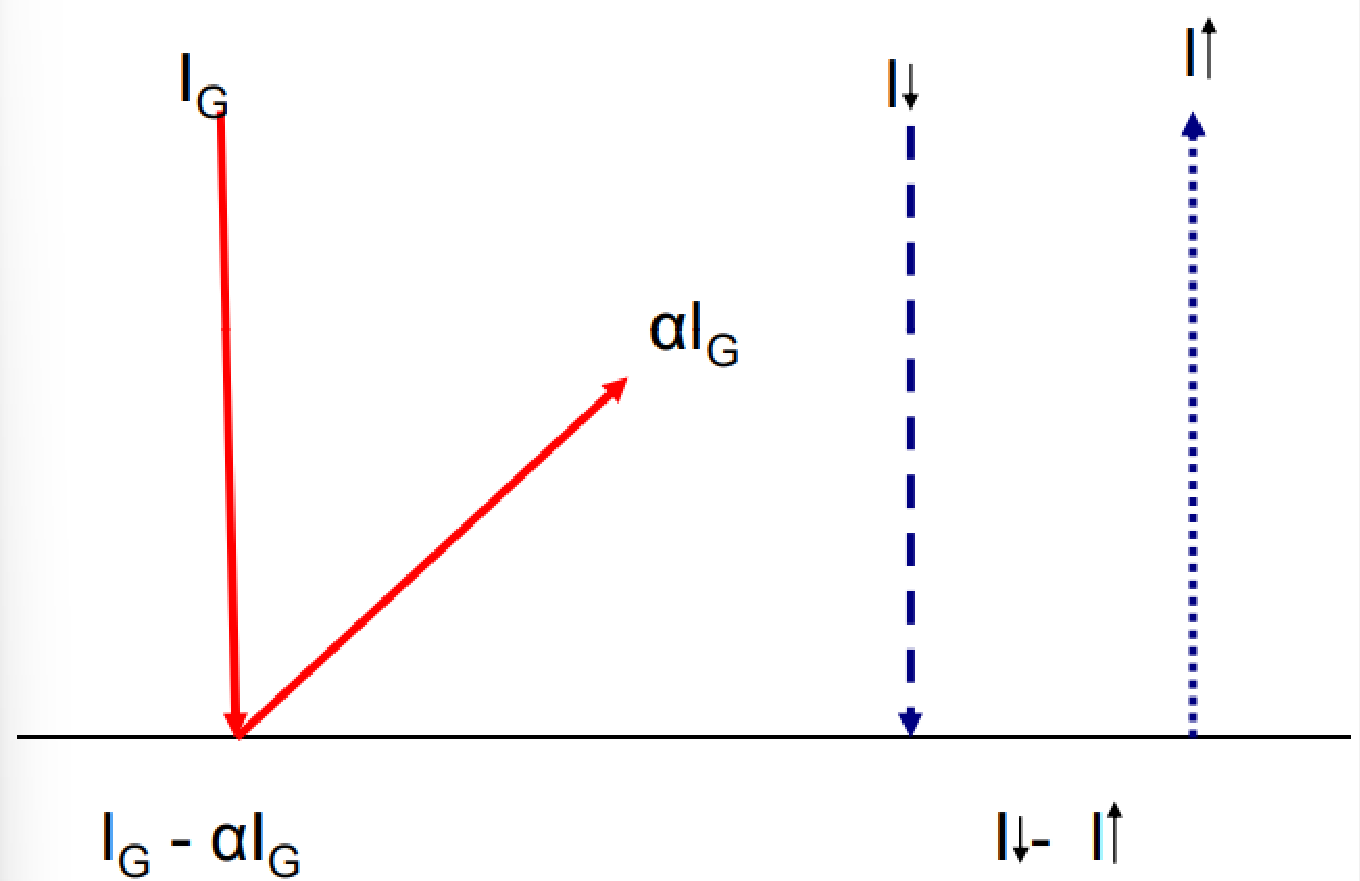
\includegraphics[width=0.5\textwidth]{ma21.pdf}
  \caption{Balance de Radiación}
  \label{ma21}
\end{figure}
\begin{equation}
    I_N = I_G-\alpha I_G +I_{\downarrow } - I_{\uparrow }
\end{equation}
\begin{notation}
    \begin{itemize}
        \item $I_N$ en $cal\cdot cm^{-2}\cdot dia^{-1}$
        \item $I_G$
        \item $I_{\downarrow }$
        \item $I_{\uparrow }$
    \end{itemize}
\end{notation}

Flujos generados por la radiaciónc neta $I_N$ ($R_N$)
\begin{notation}
    \begin{itemize}
        \item $G$: flujo de calor sensible hacia el suelo
        \item $H$: flujo de calor sensible hacia la atmósfera
        \item $L$: calor latente de evaporación de agua        
        \item $EL$: Relación de evaporación
    \end{itemize}
\end{notation}

\subsubsection{Estimación de la evaporación}

Sí se conoce la radiación radiación neta que posee una superficie superficie de agua libre (suelo húmedo) o un cultivo bien dotado de agua se puede conocer la evaporación $(E)$ de la primera o la evapotranspiración $(ET)$ del segundo con la siguiente relación:
\begin{notation}
    \begin{itemize}
        \item $E=I_N/L$
        \item $E$ en $cal\cdot cm^{-2}\cdot dia^{-1}$
        \item $I_N$ radiación neta en $cal\cdot cm^{-2}\cdot dia^{-1}$
        \item $L$: calor latente de evaporación de agua en $cal\cdot g^{-1}$      
    \end{itemize}
\end{notation}
La $L$ se calcula con la siguiente relación:
\begin{equation}
    L = 595.9 - 0.51T
\end{equation}
$T$ en $^{\circ}C$

\subsection{Radiación}
Se distinguen tres efectos que son:
\begin{itemize}
    \item Cantidad de radiación
    \item Calidad de la luz
    \item Fotoperiodo
\end{itemize}
En condiciones óptimas, que no existan ningún tipo de deficiencias, quien define la producción potencial de los cultivos.
\begin{figure}[h!]
\centering
  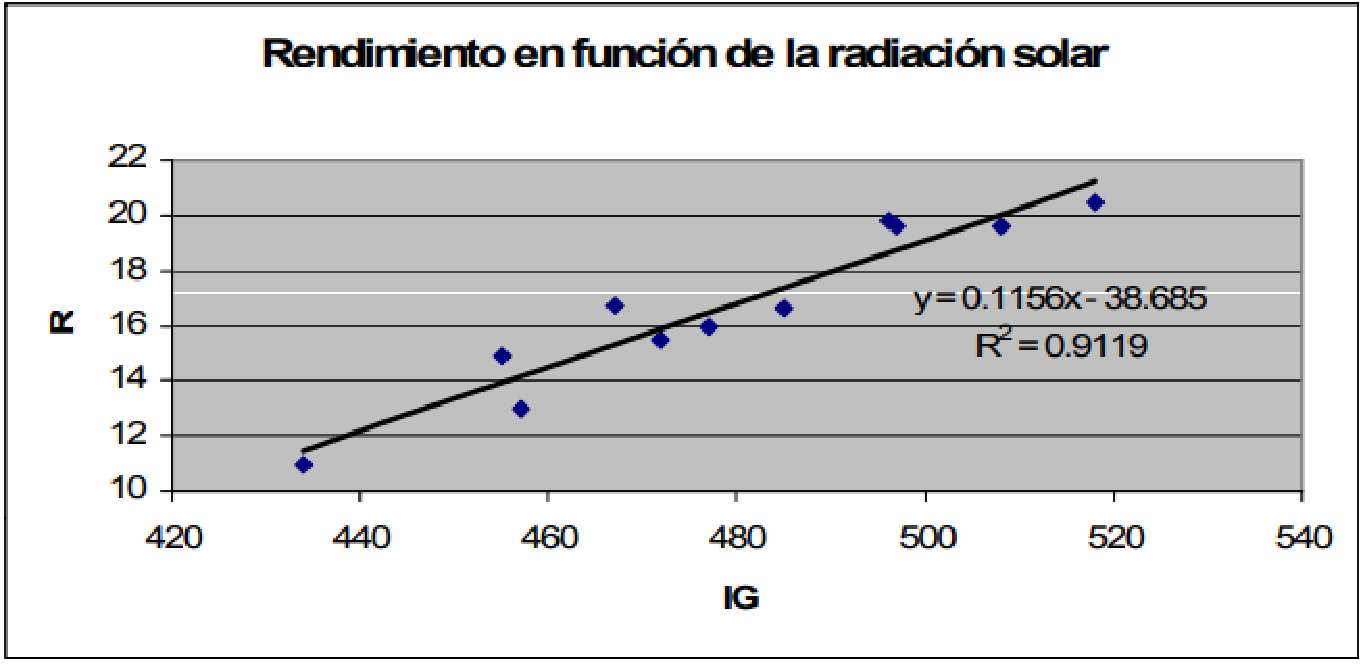
\includegraphics[width=0.5\textwidth]{ma22.pdf}
  \caption{Rendimiento en función de la radiación solar}
  \label{ma22}
\end{figure}

\subsubsection{Calidad de la luz}

Banda 1. $\lambda > 1 \mu m$ son aprovechadas en forma de calor.
Banda 2. $0.72<\lambda<1$
\begin{itemize}
    \item Crecimiento sobre las plantas.
    \item La región cercana a 1 es importante para el fotoperiodo, germinación germinación de la semilla, semilla, control control de la floración y coloración de frutos
    \item 
\end{itemize}
Banda 3. $0.61 < \lambda < 0 72$ . ,
\begin{itemize}
    \item esta región es absorbida fuertemente por la clorofila, 
    \item genera fuerte actividad fotosintética, 
    \item en algunos casos fuerte actividad foto periódica
\end{itemize}
Banda 4. $0.51 < \lambda < 0.61$ , muy bajo efecto fotosintético

Banda 5. $0.4 < \lambda < 0.5$, 
\begin{itemize}
    \item fuertemente fuertemente absorbida por los pigmentos amarillos y la clorofila 
    \item gran actividad fotosintética
\end{itemize}

Banda 6. $0.32 < \lambda < 0.4$, efectos de formación, plantas más bajas y gruesas

Banda 7. $0.28 < \lambda < 0.32$, ocasiona daños en la mayoría mayoría de las plantas

Banda 8. $\lambda < 0.28$, efectos letales rápidos en las plantas.

\subsubsection{Fotoperiodo}
la duración astronómica astronómica del día es importante en varios procesos uno de estos es la floración

Las prácticas agronómicas para el mejor aprovechamiento de la radiación solar:
\begin{enumerate}
    \item Fechas de siembra
    \item Densidad de población 2. Densidad de población
    \item Orientación de surcos. Norte - Sur más y es te-oes te menos
    \item aclareos y podas 
\end{enumerate}
\begin{figure}[h!]
\centering
  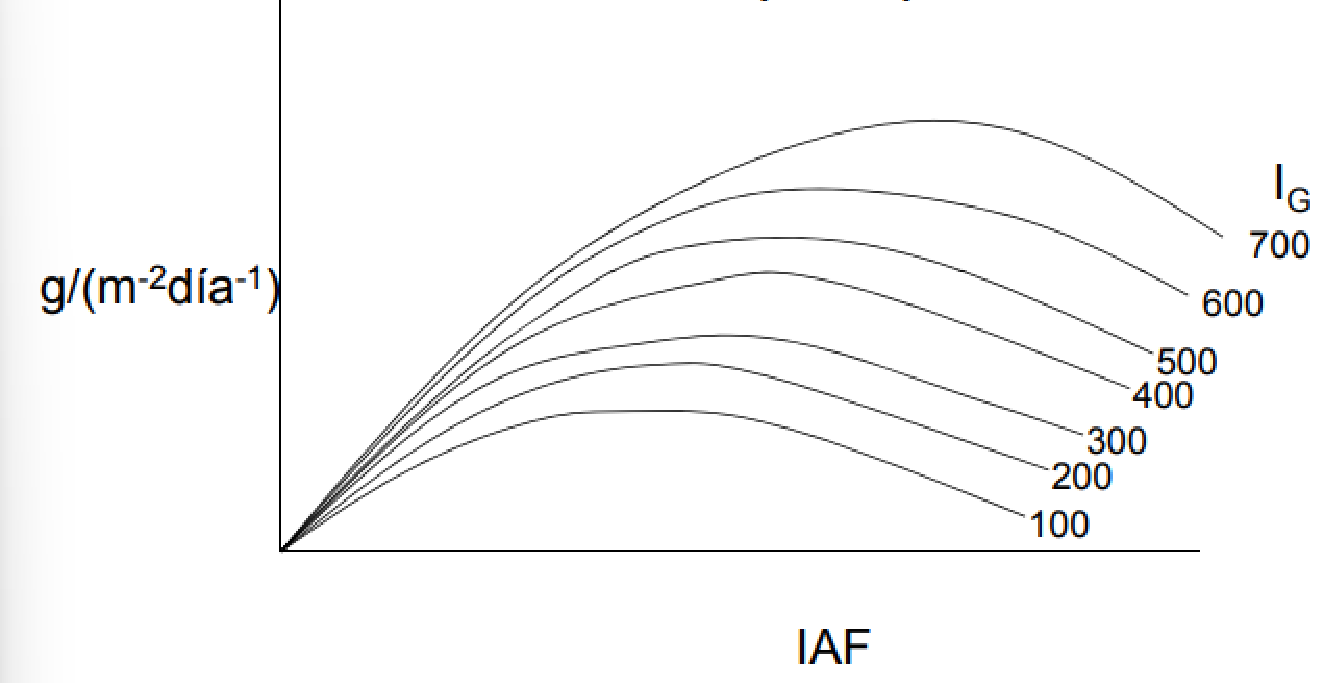
\includegraphics[width=0.5\textwidth]{ma23.pdf}
  \caption{Crecimiento en función de la radiación global y el índice de área foliar (IAF)}
  \label{ma23}
\end{figure}

\section{Temperatura}

\begin{definition}[Temperatura]
    Indica que tan caliente o frío está un cuerpo con respecto a ciertos puntos fijos: ebullición y fusión del agua
\end{definition}
\begin{definition}[Calor]
    Es energía en proceso de transferencia
\end{definition}
Es uno de los elementos principales que controlan el crecimiento y desarrollo de las plantas.

Determina la distribución espacial (geográfica) de los cultivos perennes y anuales, y de los últimos su distribución temporal.
\begin{figure}[h!]
\centering
  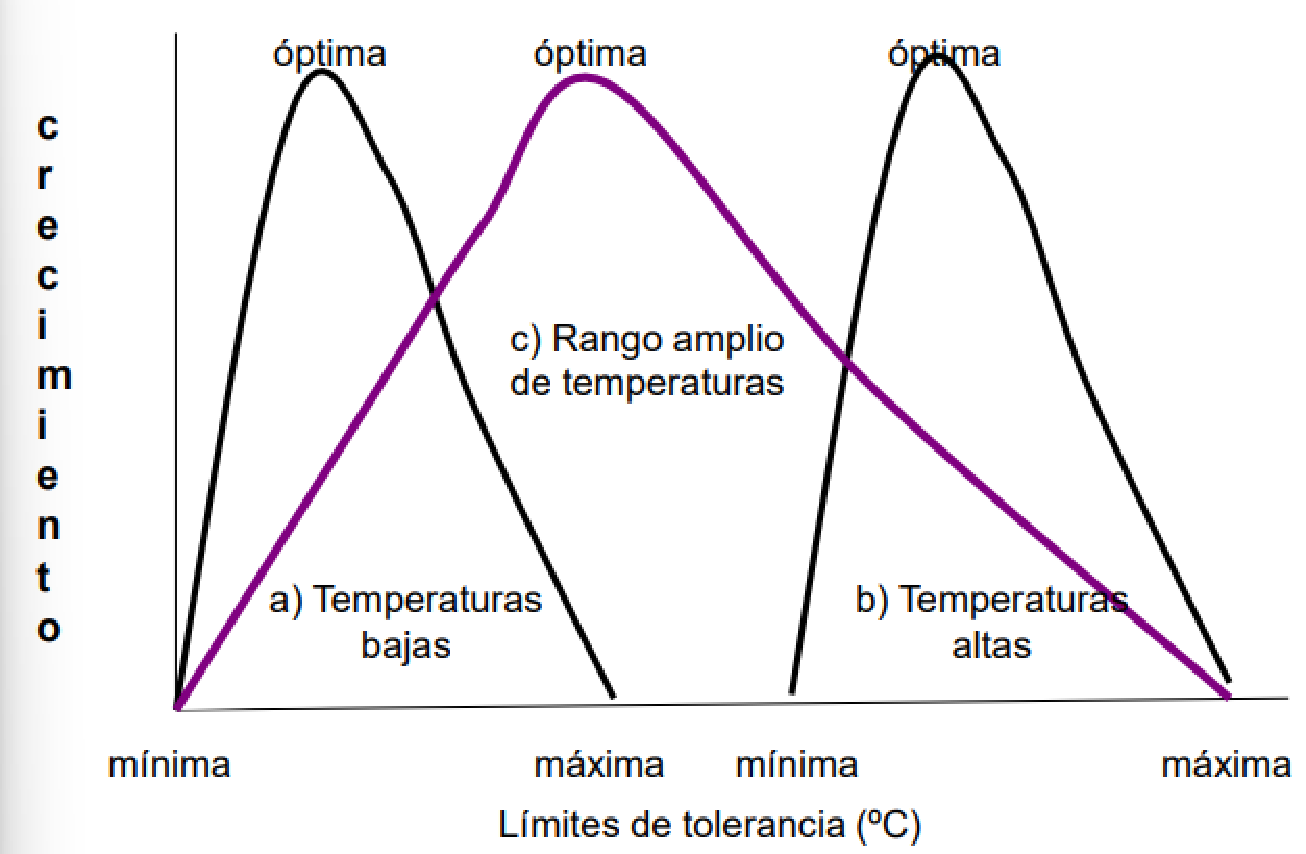
\includegraphics[width=0.5\textwidth]{ma24.pdf}
  \caption{Clasificación de las plantas según su respuesta a la temperatura}
  \label{ma24}
\end{figure}
\subsubsection{Temperaturas Cardianles}

En la figura (\ref{ma24}) se observa que cada grupo tiene tres valores de temperaturas las cuales se denominan “temperaturas cardinales” y son las que determinan las respuestas de las plantas (crecimiento y desarrollo) a las variaciones de la temperatura

Lo anterior se debe a que cualquier fase para manifestarse, requiere de temperaturas adecuadas comprendidas dentro de ciertos límites
\begin{figure}[h!]
\centering
  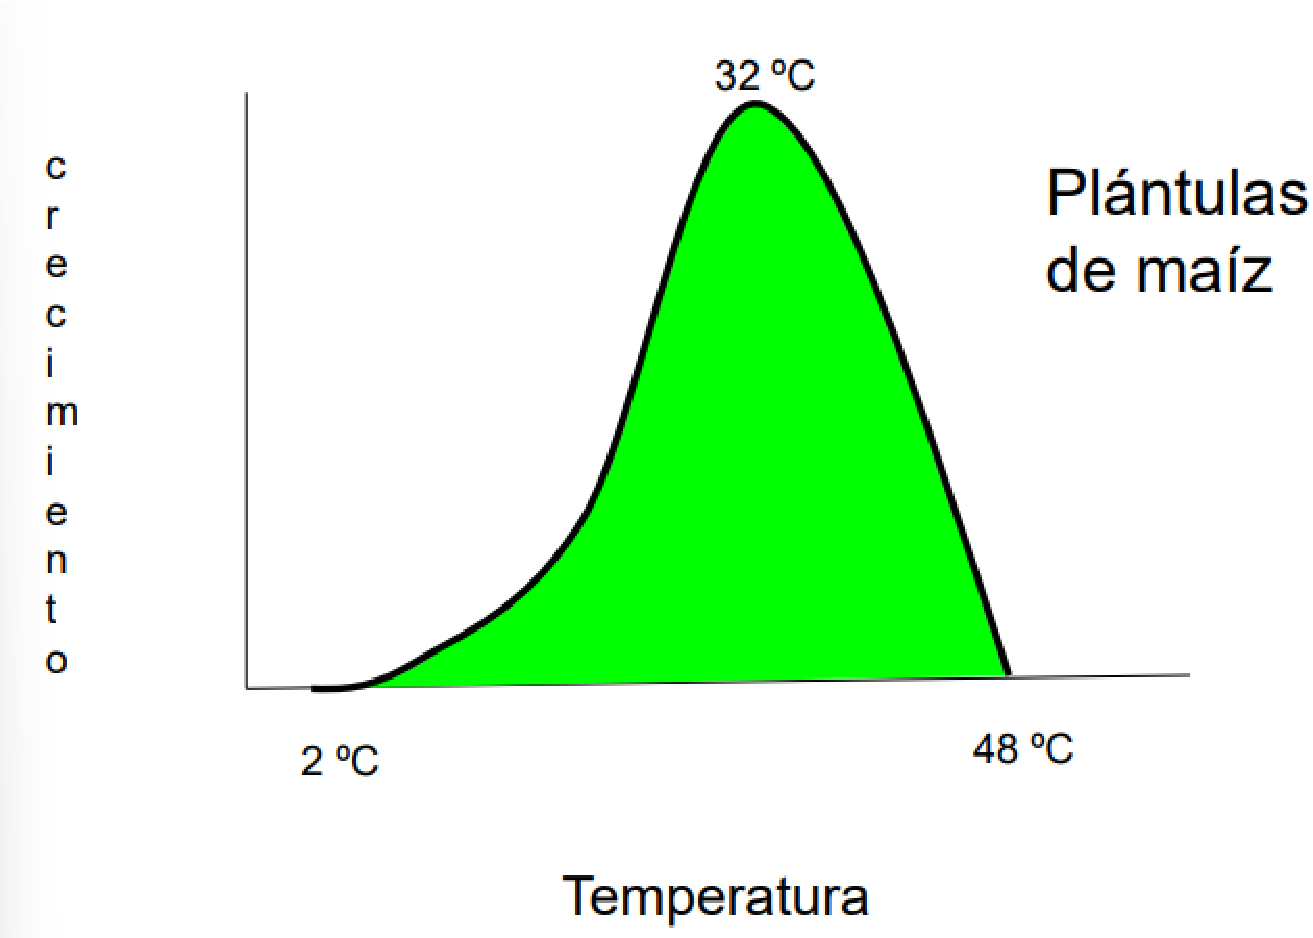
\includegraphics[width=0.5\textwidth]{ma25.pdf}
  \caption{Experiencia de Lehenbahuer}
  \label{ma25}
\end{figure}

Cuando la temperatura desciende de cierto valor mínimo se detiene el crecimiento, no obstante existen otras condiciones favorables como: humedad del suelo, nutrientes adecuados, etc. Además arriba de cierto valor máximo este crecimiento se detiene Entre estos dos valores hay un rango óptimo en el cual el crecimiento y desarrollo se efectúan a mayor velocidad debido a que representan las condiciones óptimas del cultivo
\begin{figure}[h!]
\centering
  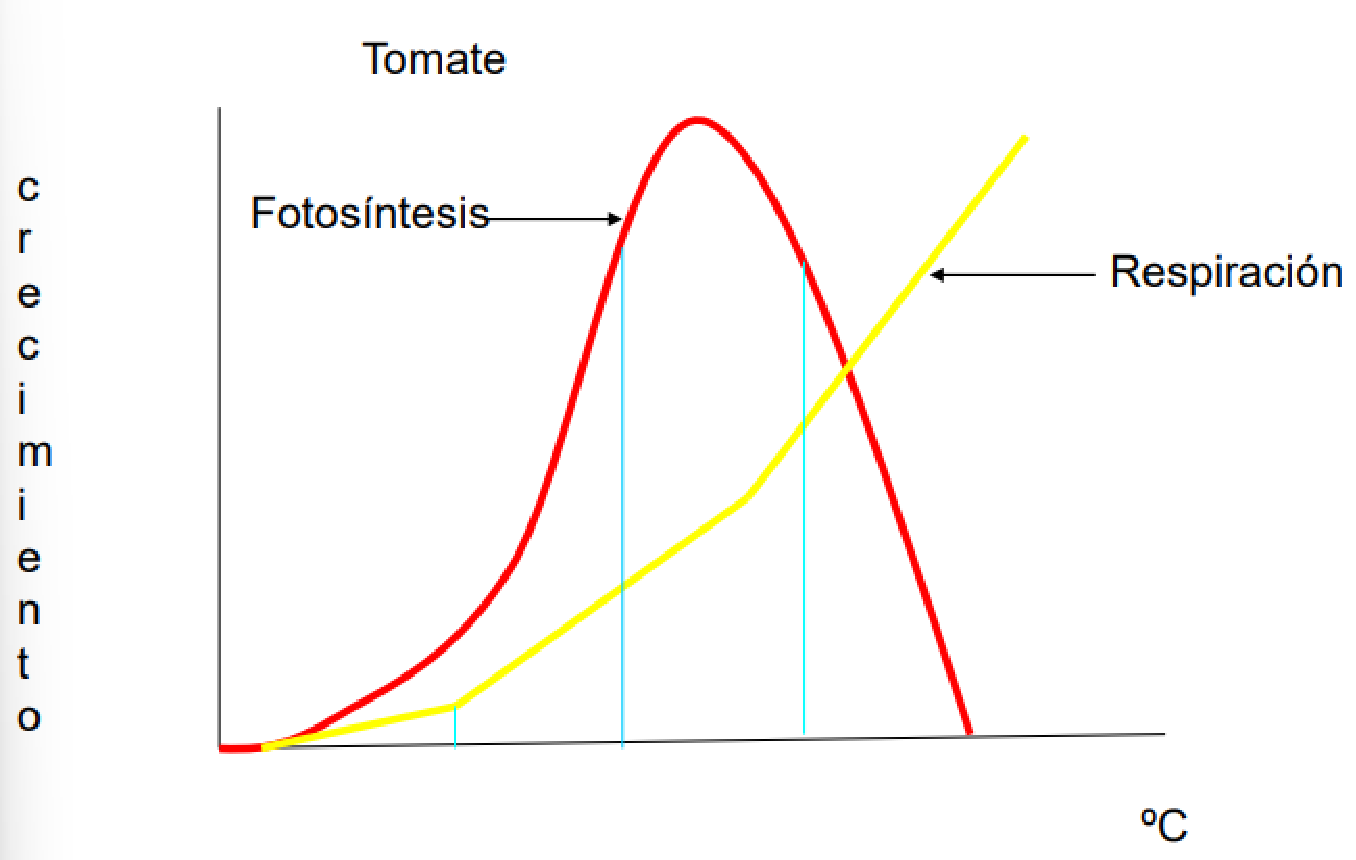
\includegraphics[width=0.5\textwidth]{ma26.pdf}
  \caption{Experiencia de Went}
  \label{ma26}
\end{figure}
En el valor mínimo y máximo el crecimiento se detiene porque la ganancia neta resulta igual a cero (fotosíntesis menos respiración). Lo anterior se debe a que existen dos procesos antagónicos, lo que genera uno el otro lo destruye, el primero es la fotosíntesis y el segundo la respiración.
\begin{figure}[h!]
\centering
  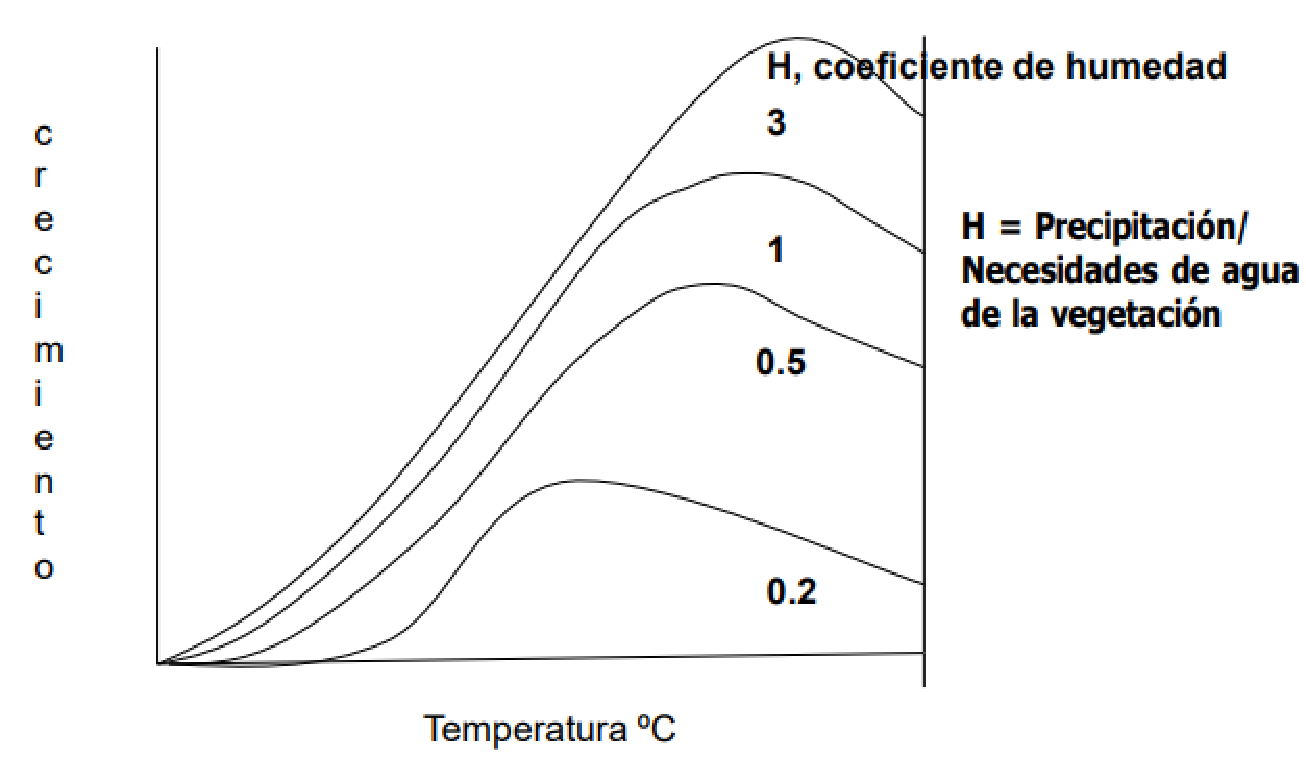
\includegraphics[width=0.5\textwidth]{ma27.pdf}
  \caption{Coeficiente de humedad (Papadakis)}
  \label{ma27}
\end{figure}
\subsubsection{Importancia de las temperaturas Cardinales}

A partir de lo anterior se deduce la importancia que tiene la temperatura en el proceso de crecimiento de los cultivos, por lo que, es importante conocer las temperaturas en las cuales un cultivo lleva a cabo sus procesos fisiológicos, ya que si se conocen éstas y se comparan con las temperaturas de una región se define su aptitud agroclimática con respecto a ese cultivo
\begin{figure}[h!]
\centering
  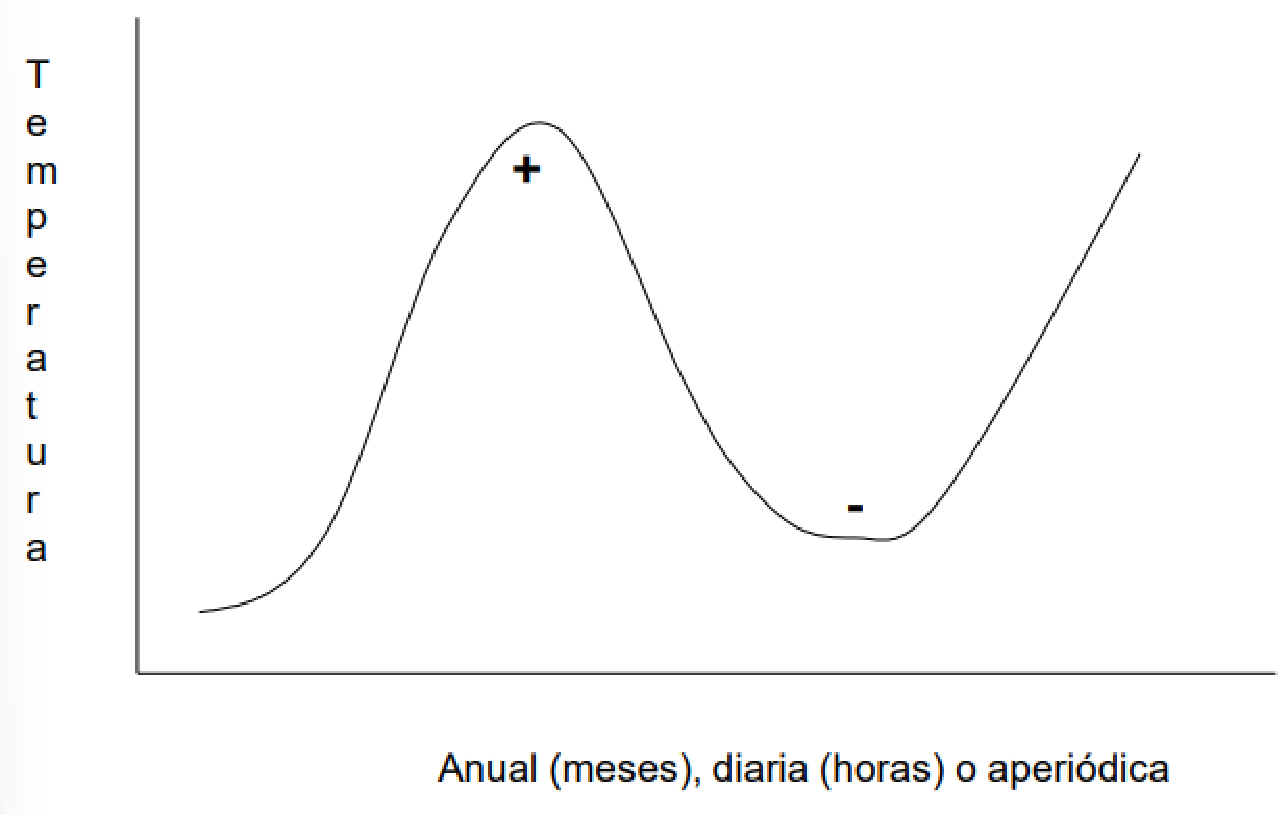
\includegraphics[width=0.5\textwidth]{ma28.pdf}
  \caption{Termoperiodo}
  \label{ma28}
\end{figure}
La variación diaria, anual o aperiódica de la temperatura del aire tiene un efecto marcado en el desarrollo de los cultivos

Dicha variación, en un ciclo completo de un año, un día o varios días, constituyen un termoperiodo anual, diario o aperiódico respectivamente. Se caracteriza por presentar dos sectores bien definidos: la termo fase positiva que corresponde al periodo más calido y la negativa al lapso más frío

\begin{definition}[Termoperiodismo]
    Las reacciones de las plantas al termoperiodo se denomina termoperiodismo y los tipos son:
    \begin{itemize}
        \item Anual
        \item Diario
        \item Aperiódico
    \end{itemize}
\end{definition}
\subsubsection{Clasificación de las plantas según su respuesta al termoperiodo anual}
\begin{enumerate}
    \item \textbf{Termocíclicas}: especies que presentan tejidos activos a la temperatura durante dos o más periodos anuales: perennes y bianuales
    \item \textbf{Paratermocíclicas}: especies anuales con tejidos activos a la temperatura en una parte de la termofase positiva y en la negativa: trigo, avena, etc.
    \item \textbf{Atermocíclicas}: Especies anuales con tejidos activos a la temperatura sólo en la termofase positiva: tomate, sorgo, maíz, etc.
    \item \textbf{Termoperiodo anual}: Distribución geográfica de los cultivos e introducción de cultivos
    \item \textbf{Termoperiodo diario}: es importante en las plantas paratermocíclicas (trigo) y atermocíclicas (tomate)
    \item \textbf{Termoperiodo aperiódico}: Interfiere en el termoperiodo anual y el diario
\end{enumerate}
\begin{figure}[h!]
\centering
  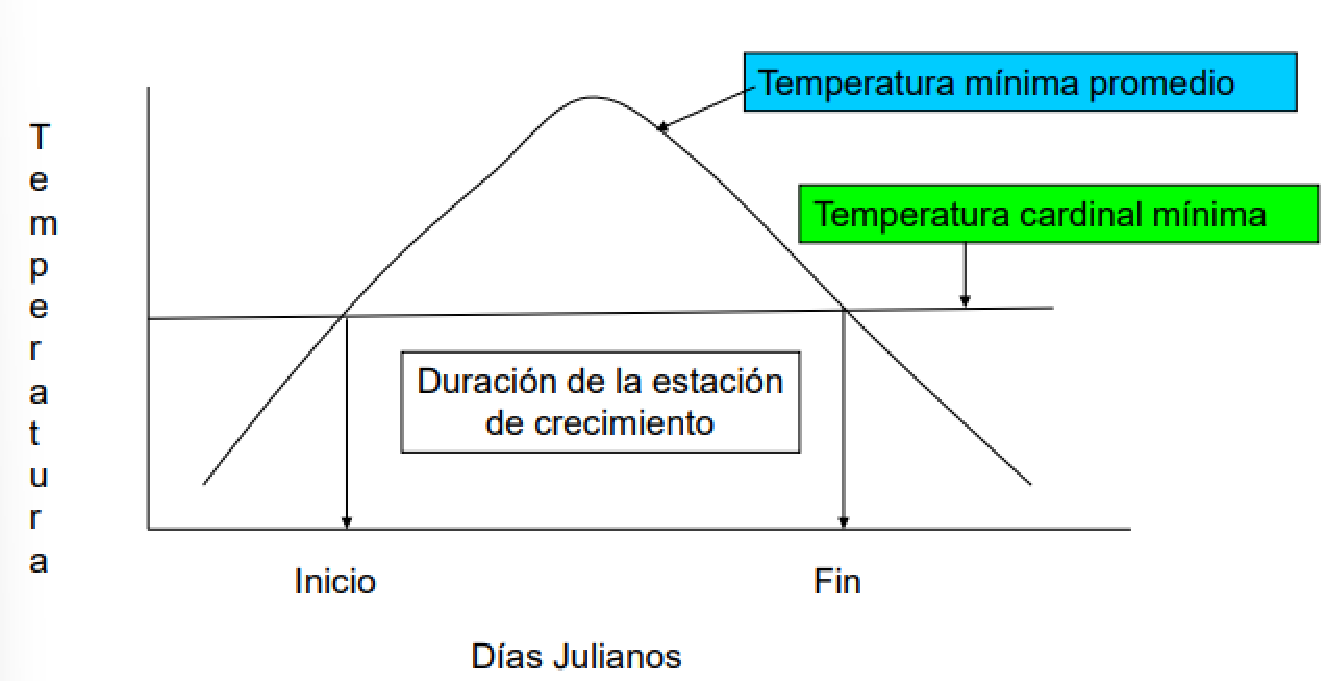
\includegraphics[width=0.5\textwidth]{ma29.pdf}
  \caption{Crecimiento}
  \label{ma29}
\end{figure}

\subsection{Grados días de desarrollo}

Cálculo de los $GDD$ y $T_b$ de un cultivo

\subsubsection{Regresión lineal}

Datos: duración en días (n) del ciclo del cultivo(emergencia-madurez fisiológica) o por etapa ysu respectiva temperatura media (T media), paravarios ciclos de cultivo

Método de cálculo: residual
\begin{align*}
    GDD=\sum\left(\bar{T}_i-T_b\right)&&\bar{T}=T_b+\frac{GDD}{n}\\
    G_D= K&&\bar{T}  Y_T\implies T_b =a_T\\
    GDD=\left(\bar{T}_1- T_b\right) +\left(\bar{T}_2- T_b\right)+\dots +\left(\bar{T}_n- T_b\right)&& \frac{1}{n}= X_t\implies GDD=b_t\\
    G_D=\left(\bar{T}- T_b\right)\cdot n&&Y_T= a_T+b_T\cdot X_T\\
    \frac{GDD}{n}=\bar{T}- T_b
\end{align*}

\subsubsection{Mínimo coeficiente de variación}

Datos: duración en días (n) del ciclo del
cultivo (emergencia-madurez fisiológica) o por
etapa y su respectiva temperatura promedio
(T), para varios ciclos de cultivo

Método de cálculo: residual
\begin{equation}
    G_D=n\left(\bar{T}- T_b\right)
\end{equation}
Se proponen varias temperaturas base $(T_b)$.

Para todos los pares de valores (T media, n) de cada ciclo de cultivo y para una temperatura base se calculan los GDD, y a éstos se le calcula la media, la desviación estándar y el coeficiente de variación

Lo anterior se repite para cada temperatura base propuesta

Los GDD y la $Tb$ que se están buscando son los que presenten el coeficiente de variación más pequeño

\subsubsection{Factores que modifican el valor de los $GDD$ y la $Tb$}
\begin{itemize}
    \item Tipo de suelo \begin{itemize}
        \item Temperatura
        \item Humedad
        \item Nivel de fertilidad
    \end{itemize}
    \item Cultivo\begin{itemize}
        \item Densidad de población
    \end{itemize}
\end{itemize}

Las aplicaciones de los GDD son: 
Programar fechas de siembra en orden a cosecha
\begin{itemize}
    \item Predecir la aparición de cada fase de desarrollo del cultivo
    \item Predecir los periodos críticos del cultivo
    \item Predicción y control de poblaciones de insectos
    \item Programación de las siguientes actividades: riego, deshierbes, fertilizaciones, polinizaciones
    \item Clasificación de especies y variedades con GDD
    \item Zonificación de cultivos en base a sus GDD
\end{itemize}

El pronóstico de la fecha de cada fase se realiza con la siguiente expresión

\begin{equation}
    FF_i=\frac{GAF_i -GAMAF_i}{GDMF_i}
\end{equation}

\begin{notation}
    \begin{itemize}
        \item $FF_i$: Fecha de la fase i
        \item $GAF_i$: Grados acumulados de la fase i
        \item $GAMAF_i$: Grados acumulados en el mes anterior donde se presenta la fase i
        \item $GDMF_i$: Grados diarios del mes donde se presenta la fase i
    \end{itemize}
\end{notation}
Los Factores que modifican los GDD de siembra a emergencia Es la profundidad a la que se realice la medición de la temperatura; La profundidad a la cual se deposita la semilla; Y la humedad del suelo

\begin{definition}[Grados días de desarrollo]
    Para indicar la duración de una etapa de un cultivo o de todo su ciclo se utiliza el número de días (tiempo civil) o los grados días de desarrollo (GDD, tiempo fisiológico).

    Es la cantidad acumulada de temperatura en cada una de las etapas de un cultivo o variedad, desde su emergencia hasta su madurez fisiológica, se expresa en $^{\circ}$-día

    Originalmente se consideró que el tiempo fisiológico (GDD) de un cultivo era el mismo en cualquier localidad, por lo que se le denomino constante térmica.
\end{definition}
\begin{example}
    Sí el valor de los GDD de un cultivo son $2500^{\circ}$- día, cual será su duración en días, de
emergencia a Madurez fisiológica, en dos
localidades que presentan las siguientes
temperaturas medias en su estación de
crecimiento: $25^{\circ}$ y $15^{\circ}$
\textit{ Sol. }
    (2500/25) = 100 días y (2500/15) = 166 días
\end{example}

Se determinó que los GDD tiene un valor a nivel regional, ya que a una misma temperatura media de dos localidades diferentes, un cultivo presenta velocidades de desarrollo diferentes: $((10+30+20)/3) = 20^{\circ}$ y $((5+40+15)/3) = 20^{\circ}$

Los grados días de desarrollo tienen dos
enfoques:
\begin{enumerate}
    \item Representa el recurso agroclimático de una región
    \item Es el requerimiento agroclimático de un cultivo
\end{enumerate}

Sí desde el momento que se produce la emergencia ($i = 1$), se suma la temperatura media de cada día hasta el momento de la madurez fisiológica ($i = n$), la suma total es siempre la misma cualquiera que haya sido la ubicación del cultivo y el año considerado.

En las sumas no se hacían intervenir las temperaturas medias menores a cero grados
\begin{equation}
    GDD= \sum_{i=1}^n \bar{T}_i\implies \bar{T}_i\geq 0^{\circ}C
\end{equation}

En el método directo se consideran como útil toda temperatura arriba de cero grados pero en realidad el crecimiento comienza con temperaturas sensiblemente más altas que la de fusión del hielo

Cada especie tiene su temperatura cardinal mínima donde se inicia el crecimiento, a este valor se le conoce también como cero vital, temperatura umbral mínima o temperatura base $(T_b)$
\begin{equation}
    GDD= \sum_{i=1}^n \left(\bar{T}_i-T_b\right) \mid \bar{T}_i <T_b\implies  \bar{T}_i-T_b =0
\end{equation}

Fisiológico (Brown, 1976) Propone la siguiente expresión en el cálculo de los GDD en el maíz:
\begin{equation}
    GDD= \sum_{i=1}^n\frac{Y_{i,\max }-Y_{i,\min}}{2}
\end{equation}

\subsubsection{Deficiencias de los métodos}
\begin{itemize}
    \item Una sola Tb en todo el ciclo del cultivo
    \item Respuesta lineal de la temperatura dando más peso a la $T_{\max}$
    \item Misma importancia a las temperaturas diurnas que nocturnas
    \item No distinguen la diferencia entre periodos calurosos o fríos
    \item No consideran las variaciones diarias de la temperatura
\end{itemize}
\subsubsection{Cálculo del recurso térmico de una región}

Generalmente se utiliza el método residual; Las $T_b$ que se consideran son: $0, 5, 10 y 15 ^{\circ}$
El recurso térmico se determina para:
\begin{itemize}
\item Todo el año
\item Estación de crecimiento por disponibilidad de temperatura
\item Periodo con bajo riesgo de helada
\item Estación de crecimiento por disponibilidad de humedad
\end{itemize}
\subsection{Eficiencia térmica}

\begin{notation}
\begin{itemize}
    \item $ETe =(IT/PTA)$
    \item $IT$, índice térmico
    \item $PTA$, puntaje teórico agroclimático en el periodo
    vegetativo del cultivo (n)
    \item $PTA = 10n$
    \item $IT = ITT_{max} +ITT_{min}$
    \item $ITT_{max}$, índice térmico por temperatura máxima
    \item $ITT_{min}$, índice térmico por temperatura mínima
    \item $ITT_{max} = \sum PAT_{max},\, i=1,\dots, n$
    \item n, duración del periodo vegetativo
    \item $ITT_{min} = \sum PAT_{min}, i=1,\dots, n$
    \item $PAT_{max}$, puntaje agroclimático por
    temperatura máxima del mes $i$
    \item $PATmin$, puntaje agroclimático por
    temperatura mínima del mes $i$
\end{itemize}
\end{notation}
Los datos de entrada son: 
Datos:
\begin{itemize}
    \item Del cultivo\begin{itemize}
        \item Temperatura cardinal mínima
        \item Temperatura cardinal máxima
        \item Temperatura óptima mínima
        \item Temperatura óptima máxima
        \item Duración del ciclo del cultivo
    \end{itemize}
    \item De la región\begin{itemize}
        \item Temperaturas promedios máximas mensuales
        \item Temperaturas promedios mínimas mensuales 
    \end{itemize}
\end{itemize}

Procedimiento:

Con la temperatura cardinal mínima ($Tc_{min}$) y la temperatura óptima mínima ($To_{min}$) se determina el puntaje agroclimático por temperatura mínima ($PAT_{min}$)

La amplitud del intervalo se define al restar la Tomin de la $Tc_{min}$ y dividirla entre cinco

La Tomin debe ser el punto medio del intervalo al que se le asigna un $PAT_{min}$ de 5

Tanto los intervalos superiores como inferiores con respecto al anterior se van degradando según la amplitud del intervalo obtenido (puede ser más o menos) hasta que la $Tc_{min}$ tiene el $PAT_{min}$ de cero

El puntaje agroclimático por temperatura máxima ($PAT_{max}$) se determina de una manera similar al $PAT_{min}$ 

\begin{example}
    Para el cultivo de sorgo, los parámetros son los siguientes:
    $Tc_{min} = 15^{\circ}$ $To_{min} = 24^{\circ}$ $Tc_{max} = 39$ $To_{max} = 30$ $n = 5$ meses
\end{example}
\textit{ Sol. }
\begin{table}[h!]
    \centering
    \begin{tabular}{@{}ll@{}}
    \toprule
    Intervalo & Puntaje \\ \midrule
    33.1-35   & 0       \\
    31.1-33   & 1       \\
    29.1-31   & 2       \\
    27.1-29   & 3       \\
    25.1-27   & 4       \\
    23.1-25   & 5       \\
    21.1-23   & 4       \\
    19.1-21   & 3       \\
    17.1-19   & 2       \\
    15.1-17   & 1       \\
    $\geq$15  & 0       \\ \bottomrule
    \end{tabular}
    \caption{Tabulación de las $PAT_{min}$}
    \label{tabma18}
\end{table}
\begin{table}[h!]
    \centering
    \begin{tabular}{@{}cc@{}}
    \toprule
    Intervalo & Puntaje \\ \midrule
    $\geq$39  & 0       \\
    37-38.99  & 1       \\
    35-36.99  & 2       \\
    33-34.99  & 3       \\
    31-32.99  & 4       \\
    29-30.99  & 5       \\
    27-28.99  & 4       \\
    25-27.99  & 3       \\
    23-25.99  & 2       \\
    21-23.99  & 1       \\
    19-21.99  & 0       \\ \bottomrule
    \end{tabular}
    \caption{Tabulación de las $PAT_{max}$}
    \label{tabma19}
\end{table}
Uniendo las tablas \ref{tabma18} y \ref{tabma19}, elaboramos una tabla con los datos de la región:
\begin{table}[h!]
    \centering
    \begin{tabular}{@{}ccccccccccccc@{}}
    \toprule
                & 1    & 2    & 3    & 4    & 5    & 6    & 7    & 8    & 9    & 10   & 11   & 12   \\ \midrule
    $T_{max}$   & 24.1 & 26.8 & 29.7 & 34.1 & 35.2 & 35.6 & 33.9 & 34.2 & 31.9 & 29.0 & 26.5 & 24.2 \\
    $T_{min}$   & 12.2 & 14.2 & 17.0 & 21.3 & 22.9 & 23.3 & 22.9 & 23.3 & 22.4 & 19.4 & 16.7 & 13.3 \\
    $PAT_{max}$ & 2    & 3    & 5    & 3    & 2    & 2    & 3    & 3    & 4    & 5    & 3    & 2    \\
    $PAT_{min}$ & 0    & 0    & 1    & 4    & 4    & 5    & 4    & 5    & 4    & 3    & 1    & 0    \\
    $IT$        & 2    & 3    & 6    & 7    & 6    & 7    & 7    & 8    & 8    & 8    & 4    & 2    \\ \bottomrule
    \end{tabular}
    \caption{Ejemplo, datos de le región}
    \label{tabma20}
\end{table}
Sumando los 5 meses con las $IT$ más altos (de junio a octubre) es 38/10(5) y esto es 0.76, al multiplicar por 100: 76\%
Esto quiere decir que la planta aprovecha el 76\& y al mismo tiempo lo que la región aporta al cultivo.

\begin{definition}[Fotoperiodo]
    Es uno de los componentes de la radiación solar y es la duración astronómica del día, desde que sale el sol hasta que se pone
\end{definition}
\begin{definition}[Fotoperiodismo]
    Es la respuesta de las plantas (floración) a la duración astronómica del día, no importa que éste haya estado nublado
\end{definition}
Se puede adelantar o atrasar la floración en condiciones naturales o en ambientes protegidos

Cuando un cultivo dispone de condiciones favorables para crecer como: temperatura, humedad edáfica, nutrientes, pero la duración del día no es adecuada para la floración, la planta crece indefinidamente produciendo casos de gigantismo

\subsubsection{Clasificación de las plantas en base a su respuesta al fotoperiodo}
\textbf{Plantas de día largo}, $N > 14h$

\textbf{Plantas de día corto}, $N < 12h$

\textbf{Plantas de días intermedios}, $12<N< 14h$

\textbf{Plantas indiferentes a la duración del día}, donde $N$ es el fotoperiodo

\begin{definition}[Unidades fototérmicas o índice heliotérmico de Geslin (1944)]
    Es la suma de las temperaturas o grados días de desarrollo multiplicada por el fotoperiodo medio del ciclo del cultivo o por etapa fenológica y se divide entre cien. Este índice (IG) es valido únicamente en la época normal de siembra del cultivo
    \begin{equation}
        IG =\frac{\bar{N}\sum\left(\bar{T} -T_b\right)}{100}
    \end{equation}
\end{definition}
Requerimiento de temperaturas bajas para la formación de flores o Vernalización:

La vernalización es la adaptación de los cereales invernales a largos periodos de temperaturas bajas. La vernalización habilita a las plantas para entrar a la etapa reproductiva, con el inicio del desarrollo de los órganos reproductivos. Los cereales invernales requieren de una cierta cantidad de frío o vernalización para la iniciación y aceleración de la floración
\begin{figure}[h!]
\centering
  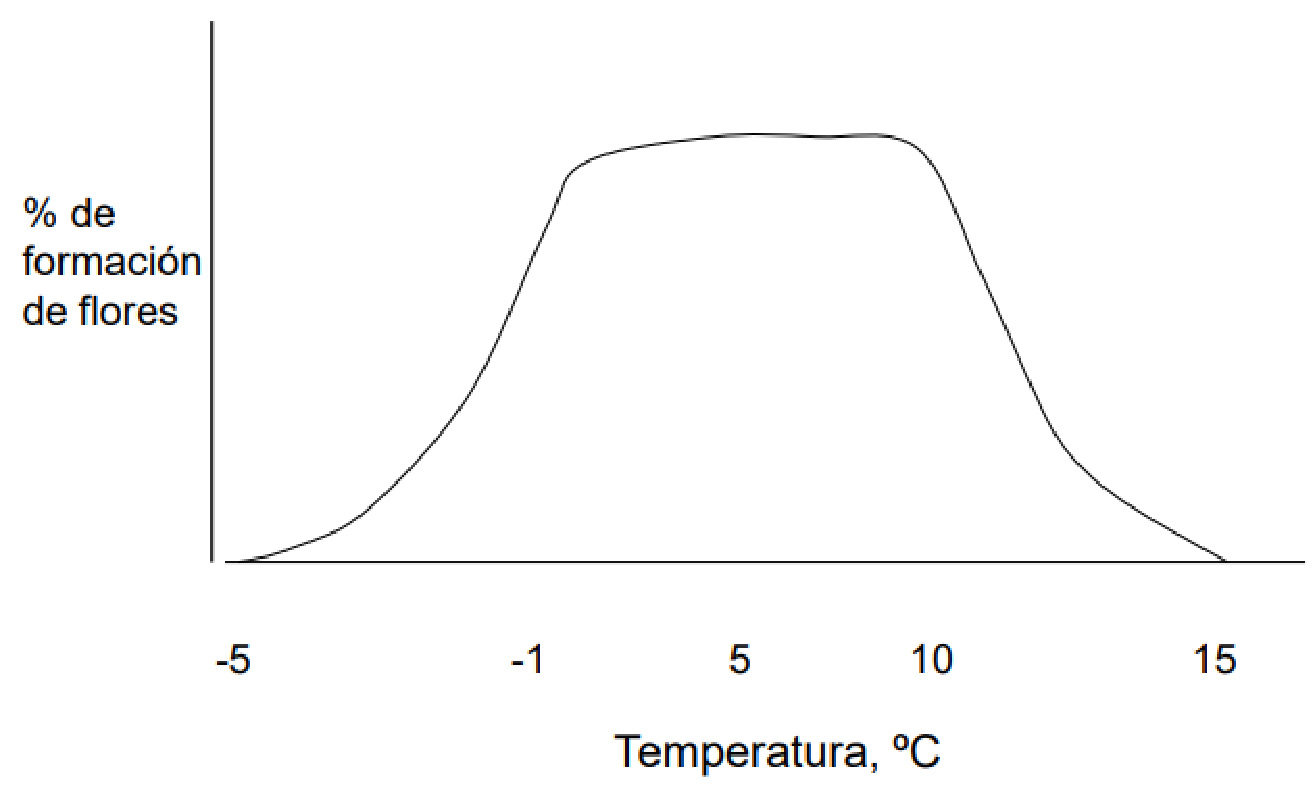
\includegraphics[width=0.5\textwidth]{ma30.pdf}
  \caption{Efecto de la temperatura durante la vernalización a la respuesta de la floración}
  \label{ma30}
\end{figure}
Esto tiene aplicaciones para el tratamiento a semillas; Nivel mínimo de agua; Periodo de activación con temperaturas altas antes del inicio del tratamiento; Presencia de oxigeno; Duración apropiada de temperaturas bajas, se presentan en el cuadro \ref{tabma21}
\begin{table}[h!]\centering
    \begin{tabular}{@{}cccc@{}}
    \toprule
    Variedades   & \begin{tabular}[c]{@{}c@{}}Temperatura\\ $(^{\circ}C)$\end{tabular} & \begin{tabular}[c]{@{}c@{}}Humedad\\ (\%)\end{tabular} & Días \\ \midrule
    Otoñales     & 0-2                                                                 & 55                                                     & 40   \\
    Semiotoñales & 3-5                                                                 & 50                                                     & 25   \\
    Primaverales & 5-10                                                                & 48                                                     & 10   \\ \bottomrule
    \end{tabular}
    \caption{Requerimiento de temperaturas bajas en diferentes variedades}
    \label{tabma21}
\end{table}
\subsection{Estimación de la temperatura}
\begin{definition}[Gradiente térmico]
    Es la disminución casi constante de la temperatura con la altura , se calcula para valores horarios, diarios, pentadales, decadales, mensuales, estaciónales o anuales
\end{definition}
\subsubsection{Estimación de la temperatura con el gradiente térmico (gt)}
Estimación de la temperatura de un lugar alto conociendo su altura, la temperatura de un lugar bajo y el gradiente térmico de la localidad

Estimación de la temperatura de un lugar bajo conociendo su altura, la temperatura de un lugar alto y el gradiente térmico de la localidad
\begin{figure}[h!]
\centering
  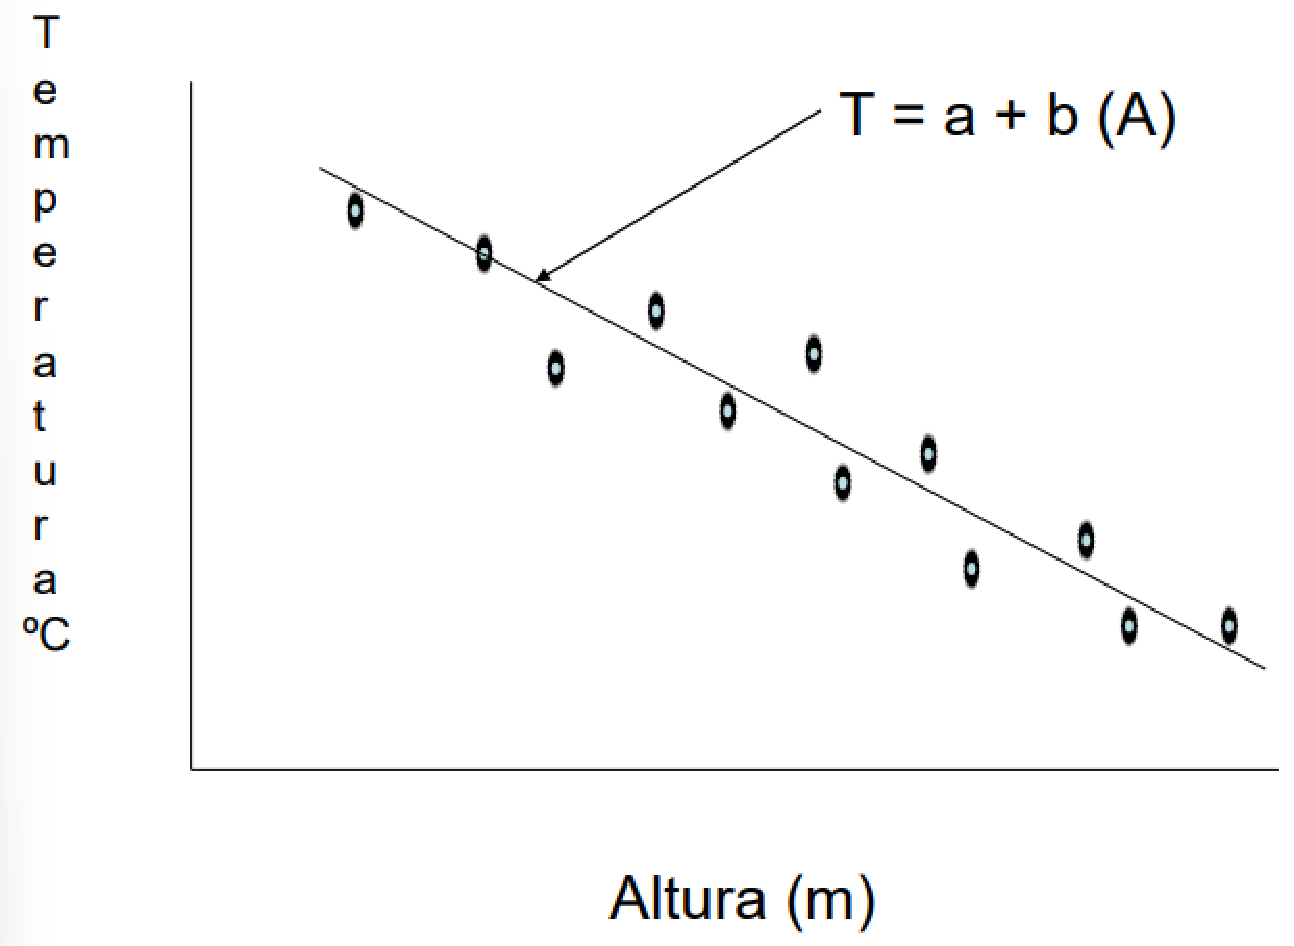
\includegraphics[width=0.5\textwidth]{ma31.pdf}
  \caption{Ecuación altotérmica}
  \label{ma31}
\end{figure}
\begin{example}
    \begin{table}[h!]
        \centering
        \begin{tabular}{@{}ccc@{}}
        \toprule
        Estación        & Temperatura $(^{\circ}C)$ & Altura (m) \\ \midrule
        Atengo          & 20.3                      & 1300       \\
        Atequiza        & 20.0                      & 1521       \\
        Autlan          & 23.3                      & 688        \\
        Mascota         & 21.0                      & 1235       \\
        Purificación    & 25.0                      & 458        \\
        Puerto Vallarta & 26.1                      & 5          \\
        Tamazula        & 21.5                      & 1127       \\
        Agostadero      & 19.0                      & 1875       \\
        Atemajac        & 15.0                      & 2065       \\
        Bolaños         & 24.4                      & 850        \\ \bottomrule
        \end{tabular}
        \caption{Ejemplo}
        \label{tabma22}
    \end{table}
\end{example}
Sirve para la estimación de la temperatura de un lugar conociendo su altura, Trazo de isotermas, Zonificación de cultivos
\begin{figure}[h!]
\centering
  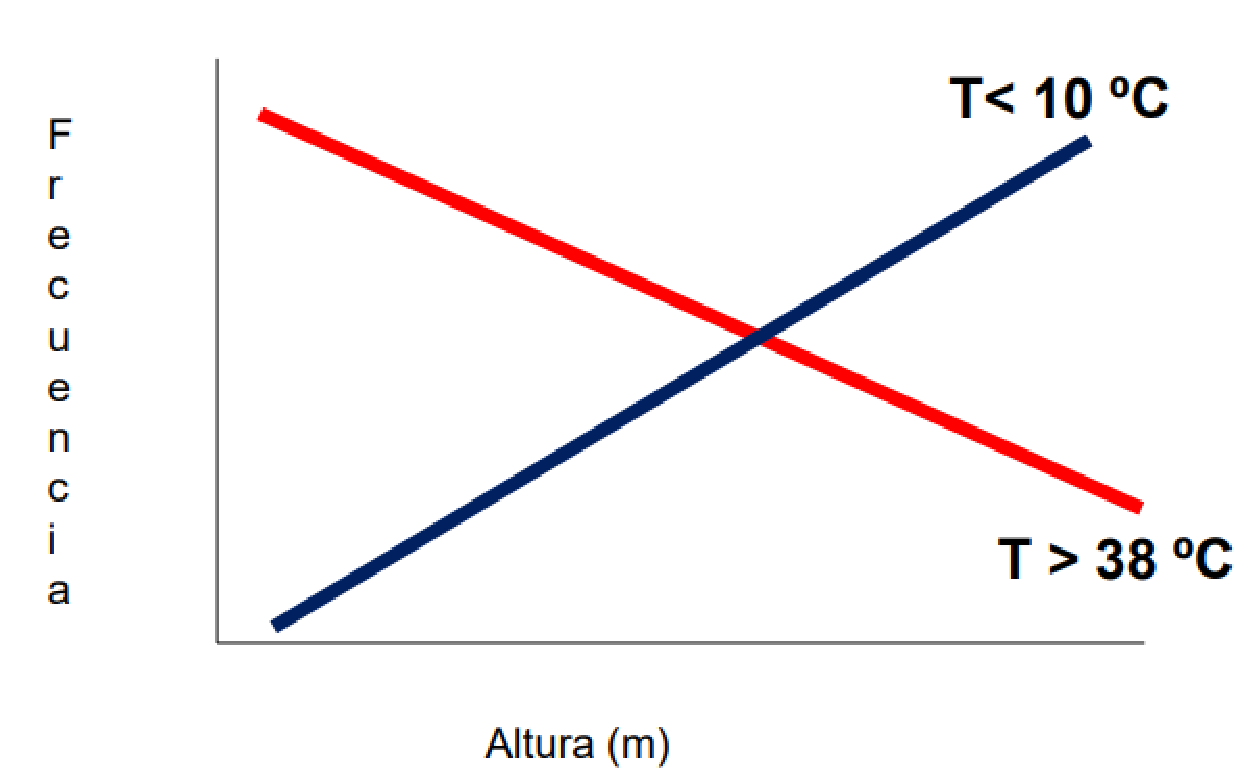
\includegraphics[width=0.5\textwidth]{ma32.pdf}
  \caption{Relaciones en temperatura máximas o mínimas}
  \label{ma32}
\end{figure}
\begin{figure}[h!]
\centering
  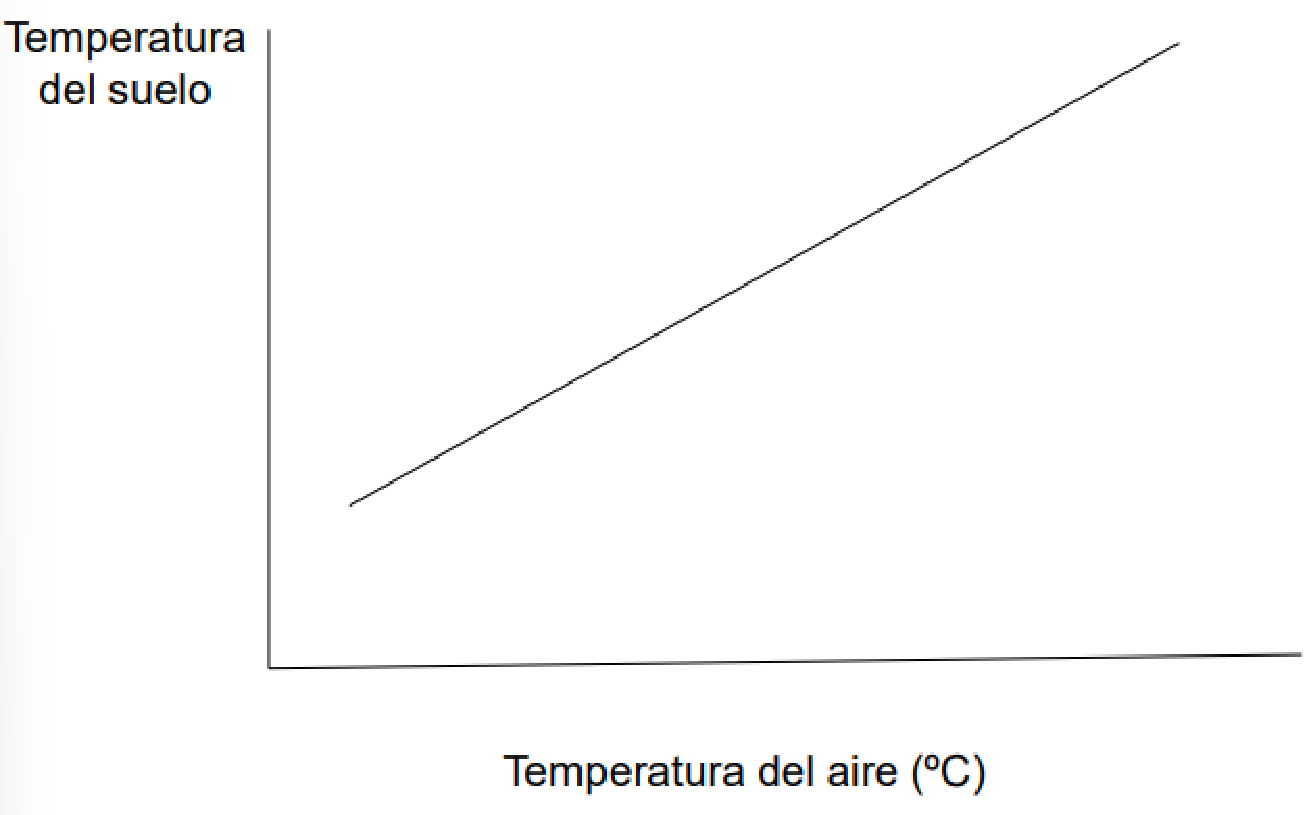
\includegraphics[width=0.5\textwidth]{ma33.pdf}
  \caption{Estimación de la temperatura del suelo}
  \label{ma33}
\end{figure}
\begin{example}
    \begin{table}[h!]\centering
        \begin{tabular}{@{}ccccc@{}}
        \toprule
            & \multicolumn{3}{c}{Profundidad (cm)} &       \\ \midrule
        Mes & 15         & 30         & 50         & Aire  \\
        1   & 13.5       & 13.2       & 18.1       & 14.88 \\
        2   & 15.4       & 14.3       & 19.2       & 16.38 \\
        3   & 18.5       & 17.2       & 21.2       & 16.61 \\
        4   & 19.7       & 18.5       & 22.6       & 19.77 \\
        5   & 19.1       & 18.7       & 22.6       & 20.17 \\
        6   & 19.0       & 18.4       & 22.3       & 19.35 \\
        7   & 17.1       & 17.2       & 21.3       & 17.28 \\
        8   & 18.0       & 17.2       & 21.7       & 17.65 \\
        9   & 18.7       & 17.2       & 21.3       & 17.67 \\
        10  & 18.0       & 16.6       & 21.2       & 17.11 \\
        11  & 17.3       & 15.6       & 20.0       & 16.29 \\
        12  & 15.6       & 14.2       & 18.7       & 15.03 \\ \bottomrule
        \end{tabular}
        \caption{Ejemplo}
        \label{tabma23}
        \end{table}
\end{example}

\subsection{Heladas}
Práctica de la defensa pasiva o lucha indirecta
\begin{itemize}
    \item Antes de efectuarse la plantación
    \item Elección del emplazamiento
    \item Elección de especies y variedades de floración tardía    
\end{itemize}
Práctica de la defensa pasiva o lucha indirecta
\begin{itemize}
    \item B. después de efectuarse la plantación
    \item Aplicación de productos químicos
    \item Regulación del abonado \begin{itemize}
        \item Nitrogenados: no usarse antes de la floración
        \item Aplicación de micronutrientes
    \end{itemize}
    \item Tratamientos fitosanitarios
    \item Técnicas de cultivo adecuadas
\end{itemize}
¿Qué se entiende por defensa activa?

Es evitar con el suministro necesario de calor que la temperatura de los órganos vegetales descienda por debajo de la temperatura crítica que los dañaría. En resumen evitar que los cultivos alcancen su temperatura crítica. Para conseguir lo anterior Debe suministrarse el calor necesario y en el momento oportuno

Para suministrar el calor necesario se tienen diferentes métodos:
\begin{itemize}
    \item Sistemas de defensa por calor húmedo
    \item Riego rodado
    \item Calor específico del agua
\end{itemize}
\subsubsection{Sistemas de defensa por calor seco}
\begin{itemize}
    \item Combustiones libres
    \item Combustiones forzadas
    \item Ventiladores
    \item Ventiladores con estufas
    \item Espumas
    \item Helicópteros
\end{itemize}

\subsubsection{Análisis probabilístico de las fechas de ocurrencia de la última y primera helada del año y del período con bajo riesgo de heladas (estación de crecimiento de los cultivos)}
\begin{itemize}
    \item Serie de observaciones en orden cronológico
    \item Se ordenan de la fecha menor a la mayor
    \item A cada fecha se le asignan un número de orden Ki en orden creciente correspondiéndole a la menor el No. 1 y así sucesivamente.
    \item Cálculo de la probabilidad empírica u observada.
\end{itemize}
En caso de Heladas primaverales:
\begin{notation}
    \begin{itemize}
        \item $P_p = I_p * C_p$
        \item $P_P=$ Probabilidad empírica de una fecha de helada primaveral; (Tardías)
        \item $I_P=$ Índice de cálculo
        \item $C_P=$ Constante
    \end{itemize}
\end{notation}
El procedimiento, es el siguiente:
\begin{align}
    &I_p = \frac{M_p + 1 - K_p}{M_p + 1}\\
    &C_p= \frac{M_p}{N_p}
\end{align}
Siempre que $M_p=N_p$ y $C_p=1$
\begin{notation}
    \begin{itemize}
        \item $Mp$ = Número de años con heladas
        \item $NP$ = Número de años de la serie en estudio.
        \item $KP$ = Número de orden de la fecha de ocurrencia, ordenado éstas en orden creciente 
    \end{itemize}
    \end{notation}
    Procedimiento para las Heladas Otoñales:
    \begin{align}
        &P_o=I_o\cdot C_o\\
        &I_o=\frac{K_o}{M_o+1}\\
        C_o = \frac{M_o}{N_o}\implies M_o = N_o\land C_o = 1
    \end{align}
    \begin{notation}
        \begin{itemize}
            \item $P_o =$ probabilidad empírica de una fecha de helada otoñal (Tempranas)
            \item $I_o =$ Índice de cálculo
            \item $C_o =$ Constante
            \item $M_o =$ Número de años con heladas
            \item $N_o =$ Número de años de la serie en estudio.
            \item $K_o =$ Número de orden de la fecha de ocurrencia, ordenado éstas en orden creciente
        \end{itemize}
        \end{notation}
    Cálculo de la probabilidad teórica
    \begin{enumerate}
        \item Se codifican las fechas de las heladas asignándoles a cada una el valor que le corresponde en el calendario fenológico (día juliano) (tabla 2) y este valor se denota como Xi.
        \item Se calcula para cada Xi (para los dos tipos de helada) su valor estandarizado (zi) con la siguiente relación.
        \begin{equation}
            Z_i = \frac{x_i - \bar{x}}{S}
        \end{equation}
        \item Con el valor estandarizado $(Z_i)$ se entra a la tabla de $Z$ y se obtienen la probabilidad que le corresponde, lo cual se denota como $F (Z_i)$.
        \item La probabilidad para las heladas primaverales es $F(P_i) = (1-F(Z_i))C_p$ esto se realiza para cada fecha.
        \item La probabilidad para las heladas otoñales es $F(Oi) = F (Zi) Co$. 
        \item Se obtienen las diferencias absolutas de $P_P- F(P_i)$ y $P_o-F(O_i)$
        \item Determinación de la fecha de la última helada tardía como de la primera temprana con un 20\% de probabilidad de ocurrencia.
    \end{enumerate}

    \begin{figure}[h!]
        \centering
          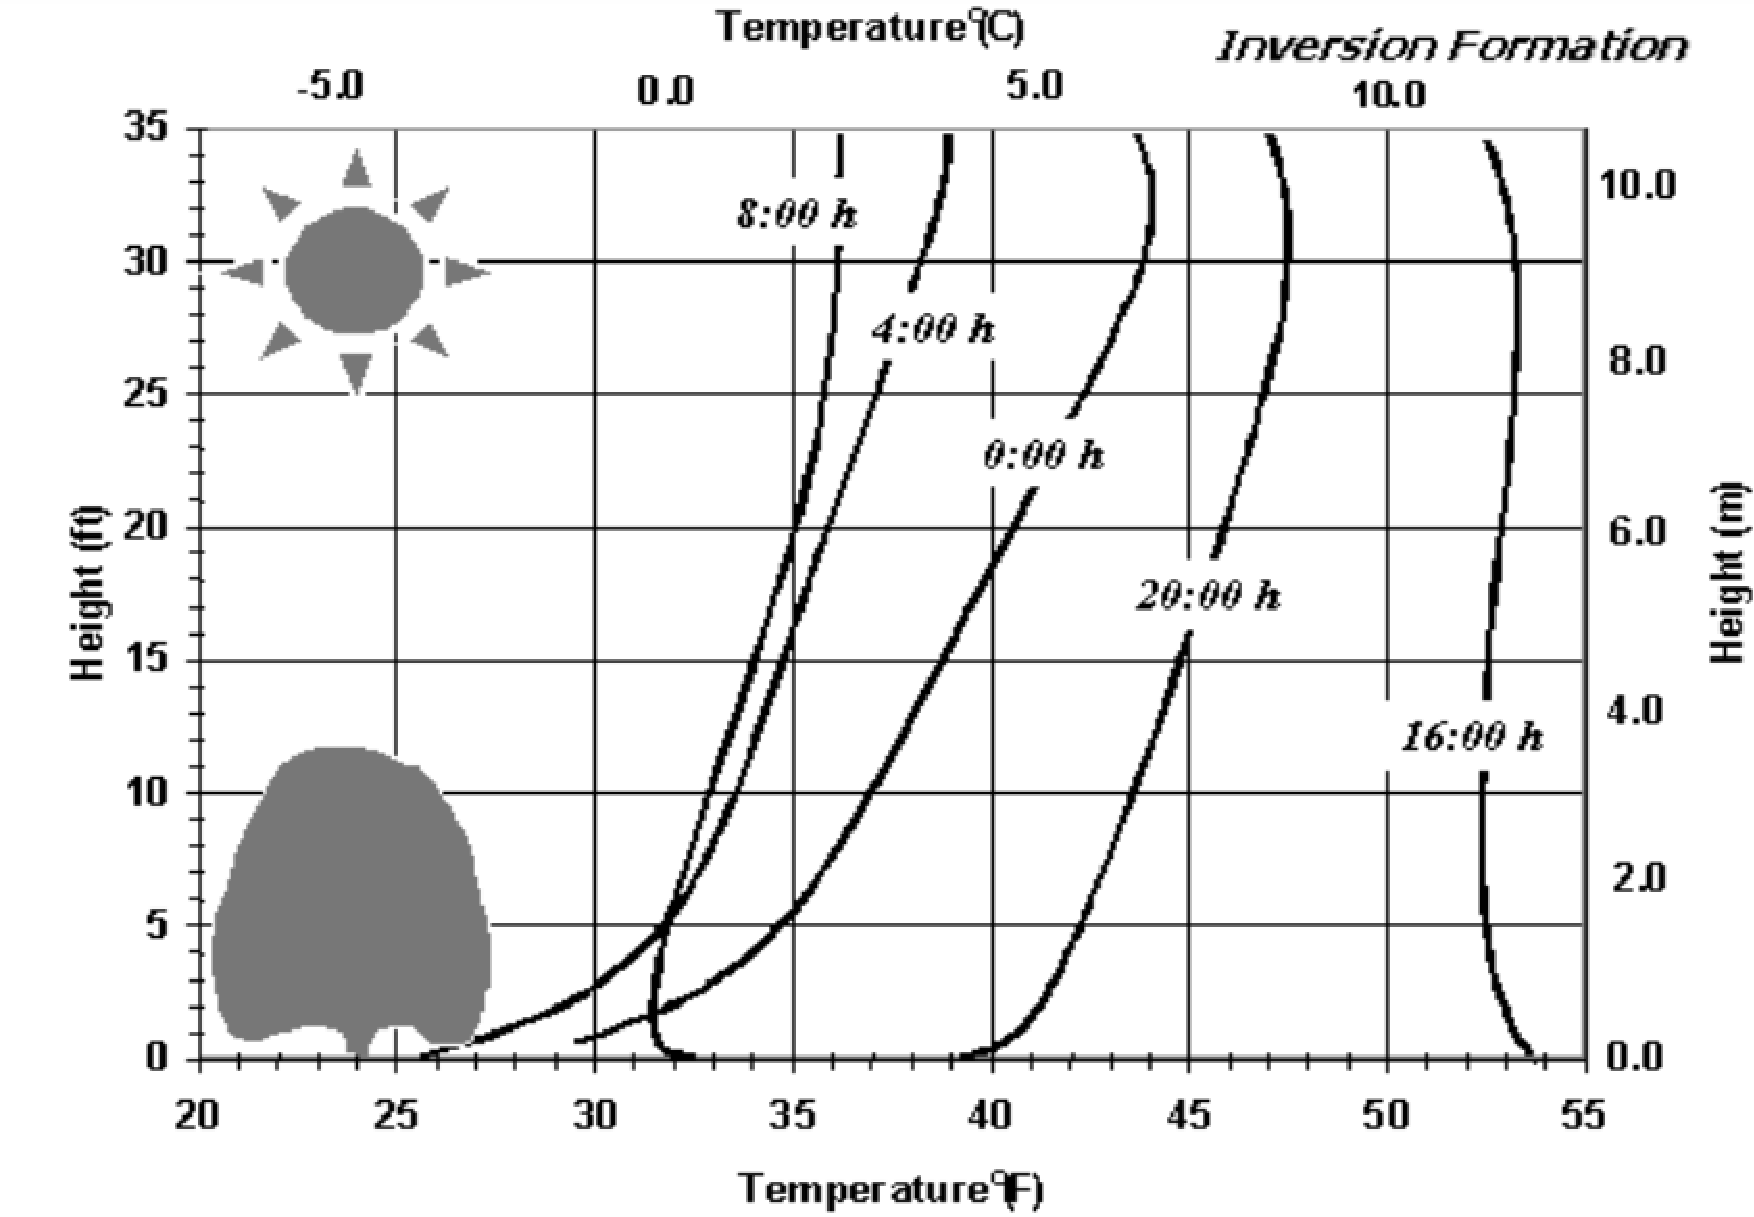
\includegraphics[width=0.5\textwidth]{ma34.pdf}
          \caption{Comportamiento de la temperatura en la noche}
          \label{ma34}
        \end{figure}
        
        
        \begin{definition}[Meteorológica]
            es la ocurrencia de temperaturas $\leq$ a 0$^{\circ}C$, medidas a una altura de 1.5 m en la caseta meteorológica
        \end{definition}
        \begin{definition}[Agrícola]
            Cuando se presentan temperaturas tan bajas que producen daños en los tejidos vegetales o la muerte de las plantas
        \end{definition}
        \begin{definition}[Socioeconomica]
            Es un descenso de temperatura que afecta el rendimiento de los cultivos ocasionando considerables pérdidas económicas y problemas sociales a los agricultores de una región
        \end{definition}
        
        \subsubsection{Efectos de las heladas}
        
        Pueden ser daños a \textbf{nivel celular} de las cuales derivan:
        
        \textbf{Fenómeno de congelación}: las heladas ocasionan una congelación del agua de los espacios intercelulares y acto seguido ocurre una salida de ésta del interior de las células hacia dichos espacios provocando una severa deshidratación; \textbf{Daños mecánicos}: las células mueren a consecuencia de una helada, debido a que forman cristales de hielo en su interior, lo que ocasiona daños mecánicos y una severa deshidratación; Probablemente \textbf{precipitación de las proteínas}
        
        o a nivel \textbf{Órgano}:
        
        En la flor ocasionan la muerte de sus óvulos evitando la fecundación y la formación del fruto; y En los frutos les puede helar las semillas o marchitar o producírseles hendiduras en la pulpa, inclusive los frutos que han sufrido el efecto de las heladas disminuyen su capacidad de conservación
        
        Así, llegamos a la clasificación de las heladas:
        \begin{itemize}
            \item Por la época que se presentan \begin{itemize}
                \item Primaverales (fecha en que se presentan)
                \item Otoñales (fecha en que se presentan)
                \item Invernales (intensidad)
                \item Estivales (intensidad)
            \end{itemize}
            \item Por el fenómeno que las origina \begin{itemize}
                \item Advección
                \item Radiación
                \item Evaporación
        \end{itemize}
        \item Como se manifiestan \begin{itemize}
            \item \textbf{Blancas}: si el aire está húmedo en el momento de una helada, se forma el rocío, si la temperatura de punto de rocío es menor a 0$^{\circ}C$, si la temperatura ya es igual a 0$^{\circ}C$, este rocío se congela formándose entonces cristales de hielo dando un color blanquecino en la superficie
            \item \textbf{Negras}: si el aire está seco y el punto de rocío es una temperatura inferior de 0$^{\circ}C$, no se forman cristales ni se observa ningún signo externo de helada
        \end{itemize}
        \end{itemize}
        \begin{figure}[h!]
        \centering
          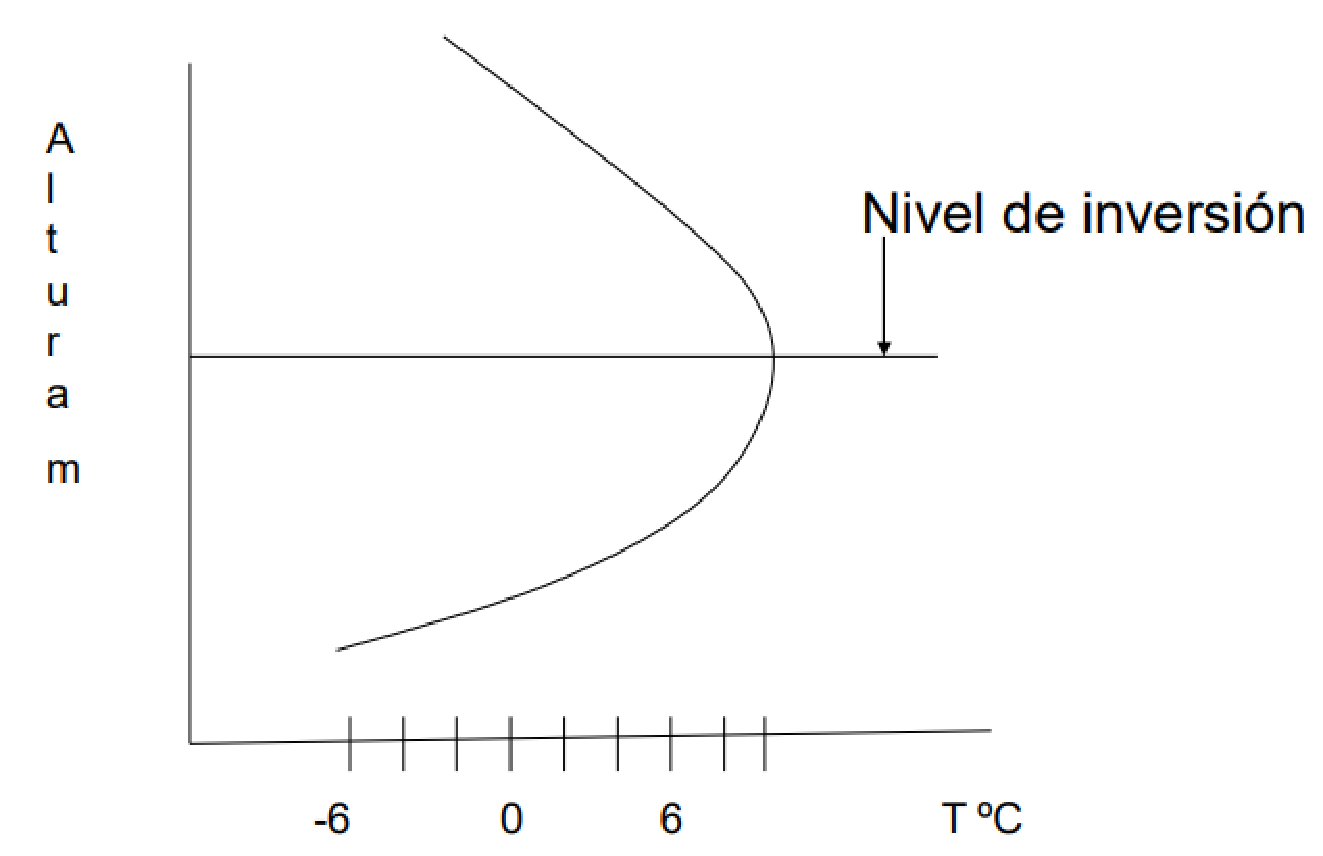
\includegraphics[width=0.5\textwidth]{ma35.pdf}
          \caption{Comportamiento típico del perfil térmico de una helada por radiación}
          \label{ma35}
        \end{figure}
        Los elementos climáticos relacionados con la helada por radiación son los siguientes:
        \begin{itemize}
            \item \textbf{Viento}: su presencia origina turbulencias que se traduce en calentamiento de las partes bajas, ya que el aire caliente situado en lo alto, desciende y se mezcla con el de las partes bajas, elevándose la temperatura, de esta forma el viento puede reducir el riesgo de una helada.
            \item \textbf{La calma} (ausencia de viento) favorece la inversión térmica, con lo que el riesgo de helada es alto
            \item \textbf{Nubosidad}: si no se presentan nubes se tiene la condición favorable para que se presente la helada
            \item \textbf{Humedad atmosférica}: si la humedad atmosférica es baja es condición favorable para que se presente una helada
        \end{itemize}
        De aquí se pueden mencionar las características del terreno relacionadas con la helada por radiación:
        \begin{itemize}
            \item La topografía
            \item Condiciones del terreno \begin{itemize}
                \item \textbf{Favorables}: sí existe vegetación en el suelo y si está recién labrado
                \item \textbf{No favorables}: suelo libre de hierbas, compacto y húmedo
            \end{itemize}
        \end{itemize}
        
        \subsection{Horas frío}
        \subsubsection{Ciclo anual de los árboles caducifolios}
        El periodo vegetativo en los árboles caducifolios año con
        año presenta una etapa de reposo, con la cual evitan las
        bajas temperaturas de la época invernal.
        
        Esta etapa de reposo se produce en los árboles caducifolios debido a que el fotoperiodo se va reduciendo y la temperatura empieza a descender.
        
        Desde el punto de vista fisiológico el árbol genera sustancias inhibidoras del crecimiento con lo cual entra en letargo.
        
        En su estado de letargo el árbol acumula frío que actúa destruyendo las sustancias inhibidoras y favorece el incremento de las promotoras, al satisfacer su requerimiento de frío rompe su estado de letargo y brota con normalidad en primavera
        
        \begin{definition}[Horas frío]
            Es la acumulación de temperaturas menores o iguales a siete grados centígrados por los frutales caducifolios en la época invernal, para salir de la etapa de reposo
        \end{definition}
        Entre los factores que modifican la acumulación de horas frío, puede mencionarse los siguientes:
        \begin{itemize}
            \item Alta oscilación térmica diaria
            \item Presencia de épocas definidas de calor durante el invierno
            \item Alta radiación solar
            \item Reducida humedad atmosférica y edáfica
        \end{itemize}
        Así como los métodos artificiales para contrarrestar las deficiencias de horas frío, por el cultivo:  Cultivo; Encalado de los árboles; Aspersión de agua; Empleo de patrones de bajas necesidades de horas frío; Podas adecuadas y oportunas; Riegos ligeros durante el invierno
        
        Es importante tener claro que al introducir una especie en una región se debe conocer tanto el requerimiento de la primera como el recurso de la segunda. ¿Qué pasa si el lugar tiene mayor cantidad de horas frío que la variedad? y/o ¿Qué pasa si se tiene la condición contraria, el lugar tiene menor cantidad de horas frío que la variedad?
        \begin{itemize}
            \item Directos \begin{itemize}
                \item Huerto fenológico
                \item Termógrafo
            \end{itemize}
            \item Indirectos \begin{itemize}
                \item Da Mota
                \begin{equation}
                    HF = \sum 485.1 - 28.52\cdot T
                \end{equation}
                Donde la sumatoria va desde el mes $i = 11$ (nov), 12 (dic), 1(ene) y 2(Feb); $HF=$ es horas frío y $T$ temperatura media mensual de cada mes
                \item Weinberger
                \begin{equation}
                    HF = 2121.85 -125.23\cdot T
                \end{equation}
                Donde $T$ es el promedio de las temperaturas medias de los meses de diciembre y enero
                \item Sharp
                \begin{equation}
                    HF = \sum 638.95 - 33.01\cdot T
                \end{equation}
                Donde la sumatoria va desde el mes $i = 12$, 1 y 2; $T$, temperatura media mensual de cada mes
            \end{itemize}
        \end{itemize}
        Para realizar un análisis probabilístico de las horas frío puede ser Con el método de la distribución normal ó con la relación de las horas frío con la altura
        \section{Evapotranspiración}
        \subsection{Terminología}
        El agua cumple en la vida de las plantas un papel muy importante,
        ya que el agua que toman con las raíces la utilizan de la siguiente
        manera:
        \begin{itemize}
            \item Una pequeña cantidad del agua pasa a formar parte de la
            composición de la materia seca
            \item Otra parte algo mayor, mantiene la hidratación de las células
            dándole rigidez a los tejidos y en consecuencia a toda la planta
            \item La mayor parte del agua que consumen las plantas es el medio de
            transporte de los elementos nutritivos necesarios en el desarrollo y
            crecimiento de las plantas y se pierde a la atmósfera por
            transpiración estomática y cuticular
            \item Propicia el intercambio gaseoso de los cultivos con la atmósfera de su entorno
            \item Es una componente fundamental del balance hídrico en determinar la disponibilidad hídrica de un sistema
            \item Hay una relación entre el consumo de agua de los cultivos y el
            rendimiento de éstos
        \end{itemize}
        
        
        \begin{definition}[Evaporación potencial $(E)$]
            Proceso físico mediante el cual una cantidad de agua en forma de vapor de agua se pierde desde una superficie de agua libre a la atmósfera a través de su cambio de estado
        \end{definition}
        
        \begin{definition}[Transpiración]
            Proceso físico-biológico mediante el cual se pierde agua en forma de vapor de agua hacia la atmósfera por medio de los estomas de las plantas
        \end{definition}
        
        \begin{definition}[Evapotranspiración $(ET)$]
            Es un proceso combinado que comprende la evaporación de todos los tipos de superficies (vegetal-suelolamina de agua) y la que transpiran las plantas
        \end{definition}
        \begin{definition}[Evapotranspiración potencial (ETP)]
            Es la máxima cantidad de agua capaz de ser perdida en forma de vapor de agua, en un clima, por una capa de vegetación verde en pleno desarrollo, de cobertura total y de corta altura, cuando no se limita la cantidad de agua suministrada al suelo
        \end{definition}
        \begin{definition}[Evapotranspiración de Referencia $(ETo)$]
            Es la máxima cantidad de agua que en forma de vapor, pierde un pasto (alfalfa) de cobertura total, en pleno desarrollo, de porte bajo y sin limitaciones de humedad edáfica
        \end{definition}
        \begin{definition}[Evapotranspiración máxima de cultivo (ETM)]
            Es la cantidad de agua que evapotranspira un cultivo dado en cualquier etapa de su ciclo y que no tiene restricción de agua en el suelo
        \end{definition}
        \begin{definition}[Evapotranspiración Real de cultivo ($ETR$)]
            Es la cantidad de agua perdida por evapotranspiración por el complejo suelo-planta-atmósfera, en las condiciones meteorológicas, edafológicas y fenológicas existentes.
        \end{definition}
        \begin{figure}[h!]
            \centering
            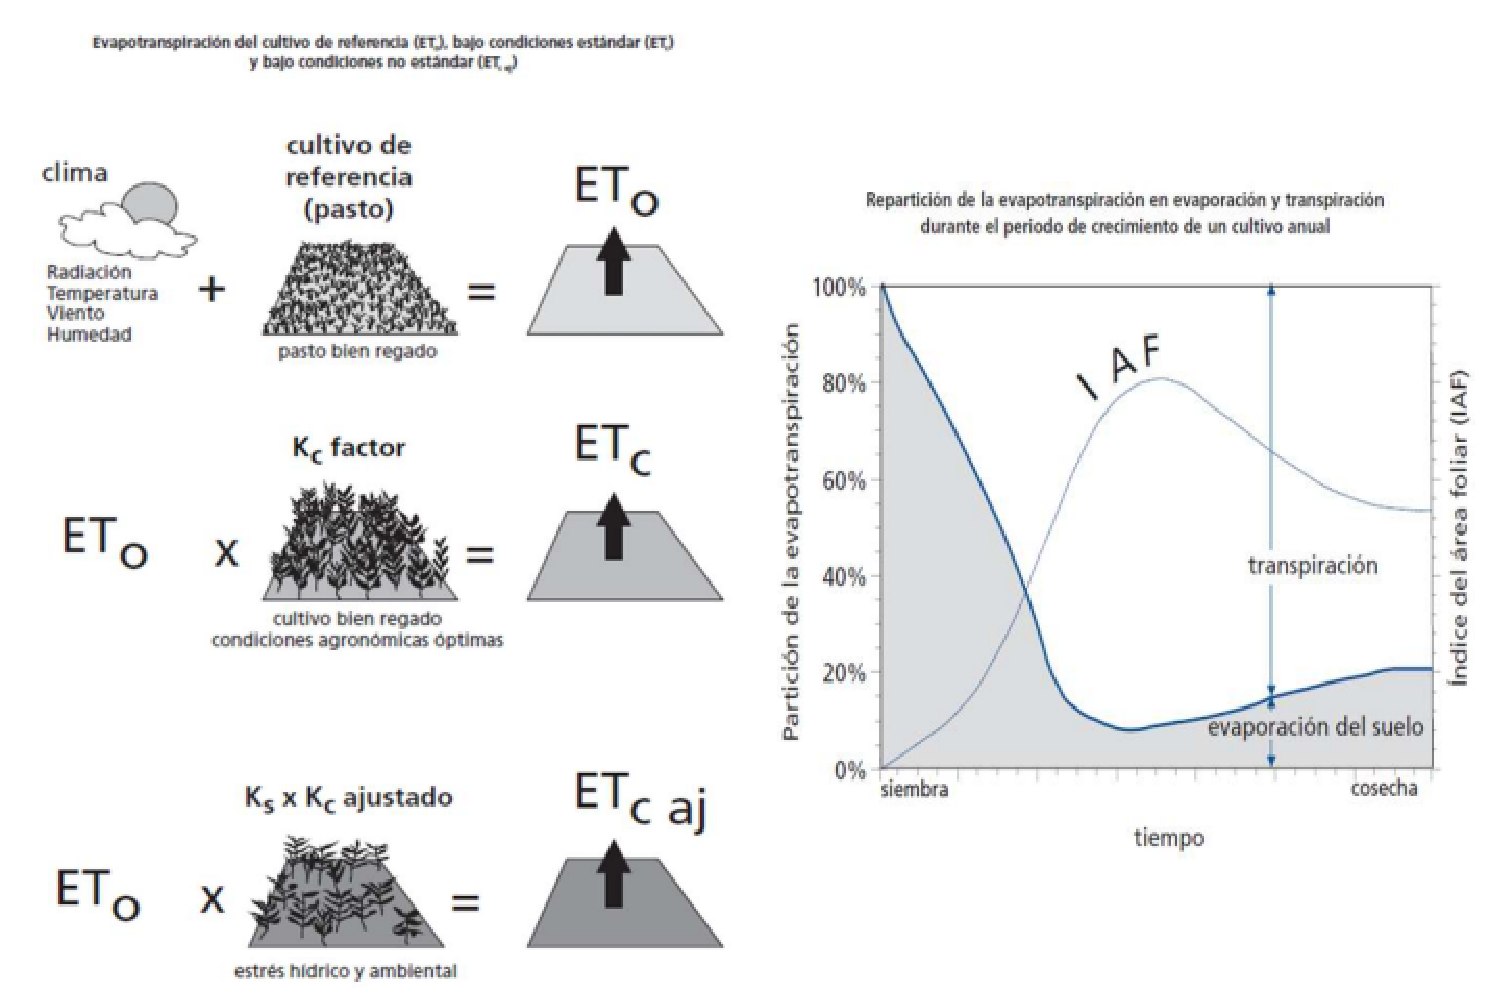
\includegraphics[width=0.5\textwidth]{ma36.pdf}
            \caption{Evapotranspiración del cultivo de referencia bajo condiciones estándar y bajo condiciones no estándar}
            \label{ma36}
        \end{figure}
        \subsubsection{Análisis de los elementos que intervienen en los procesos de evaporación y evapotranspiración}
        \begin{figure}[h!]
        \centering
          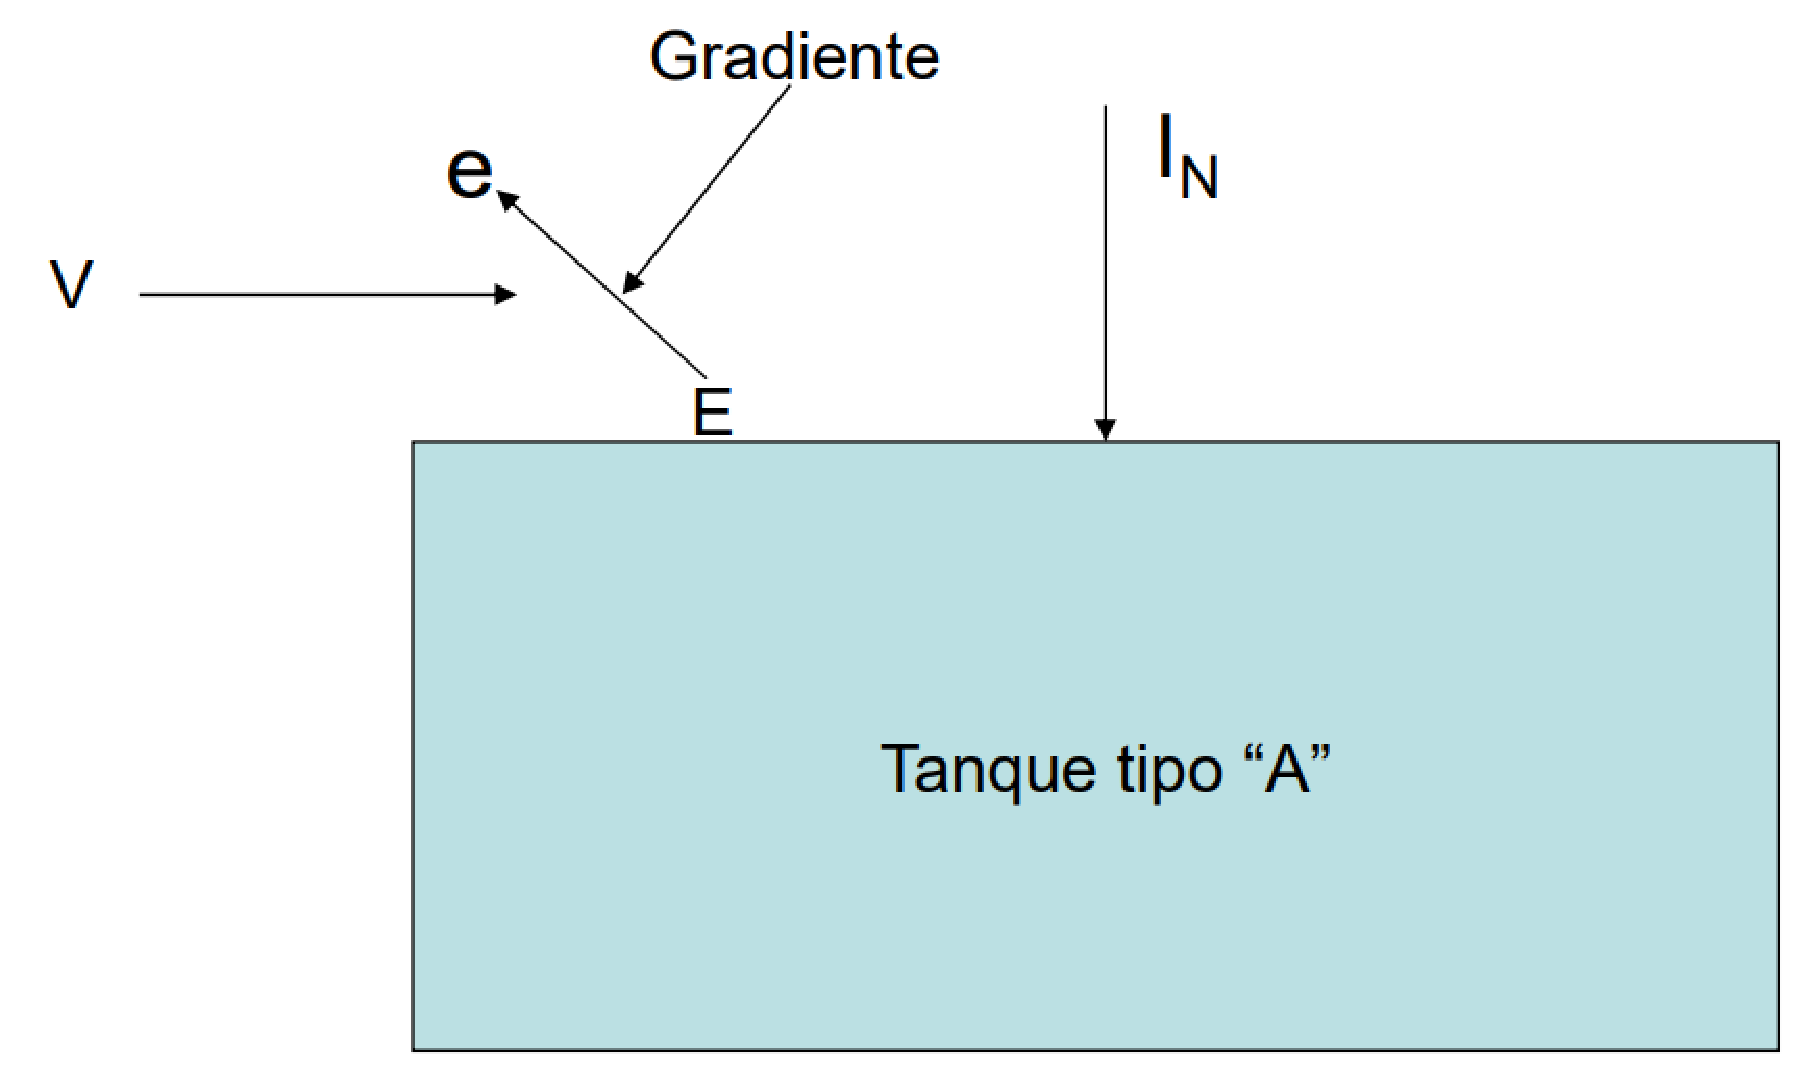
\includegraphics[width=0.5\textwidth]{ma37.pdf}
          \caption{En el proceso de evaporación es necesario destacar, los aspectos físicos que proporcionan energía en el cambio de fase del agua  }
          \label{ma37}
        \end{figure}
        Demanda (petición): Depende exclusivamente de las exigencias impuestas a cada instante por el clima
        
        Oferta: Corresponde a la cantidad de agua que el sistema suelo-planta es capaz de ceder a la atmósfera.
        
        Como se observa en la figura \ref{ma38} si el agua no es un elemento limitante en el proceso de evapotranspiración, se considera que este se comporta de forma similar a la evaporación
        \begin{figure}[h!]
        \centering
          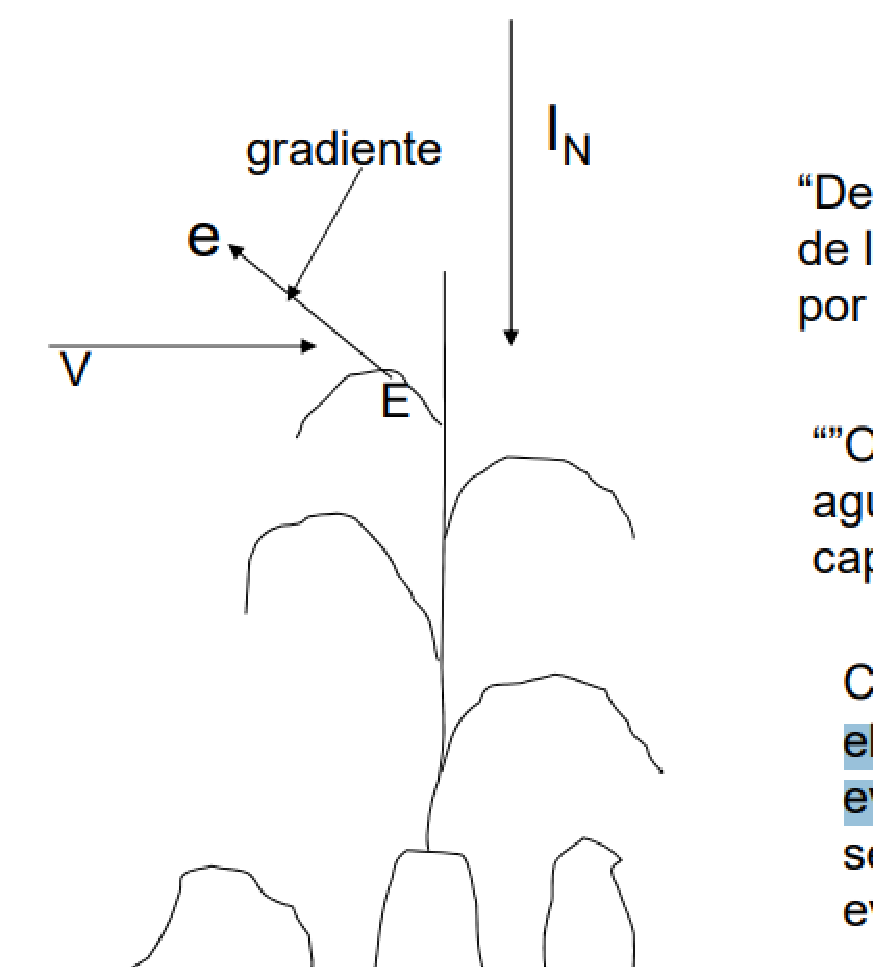
\includegraphics[width=0.5\textwidth]{ma38.pdf}
          \caption{No hay limitante de agua en el suelo}
          \label{ma38}
        \end{figure}
        
        La cantidad de agua que se pierde por evaporación depende del estado en que se encuentre en la superficie evaporante:
        \begin{itemize}
            \item Energía disponible
            \item Estado de retención del agua
            \item Índice de área foliar    
        \end{itemize}
        Como se observa en la figura \ref{ma39}, si el agua es un elemento limitante en el proceso de evapotranspiración, se considera que la planta lo regula
        \begin{figure}[h!]
        \centering
          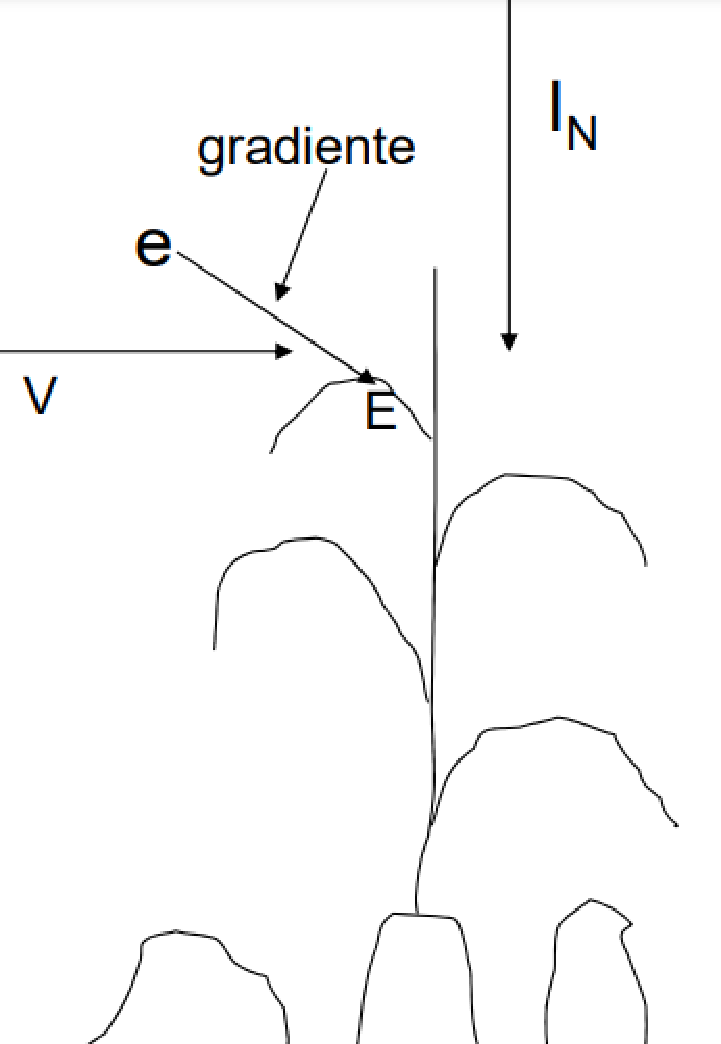
\includegraphics[width=0.5\textwidth]{ma39.pdf}
          \caption{Contenido real de agua en el suelo}
          \label{ma39}
        \end{figure}
        \begin{figure}[h!]
            \centering
              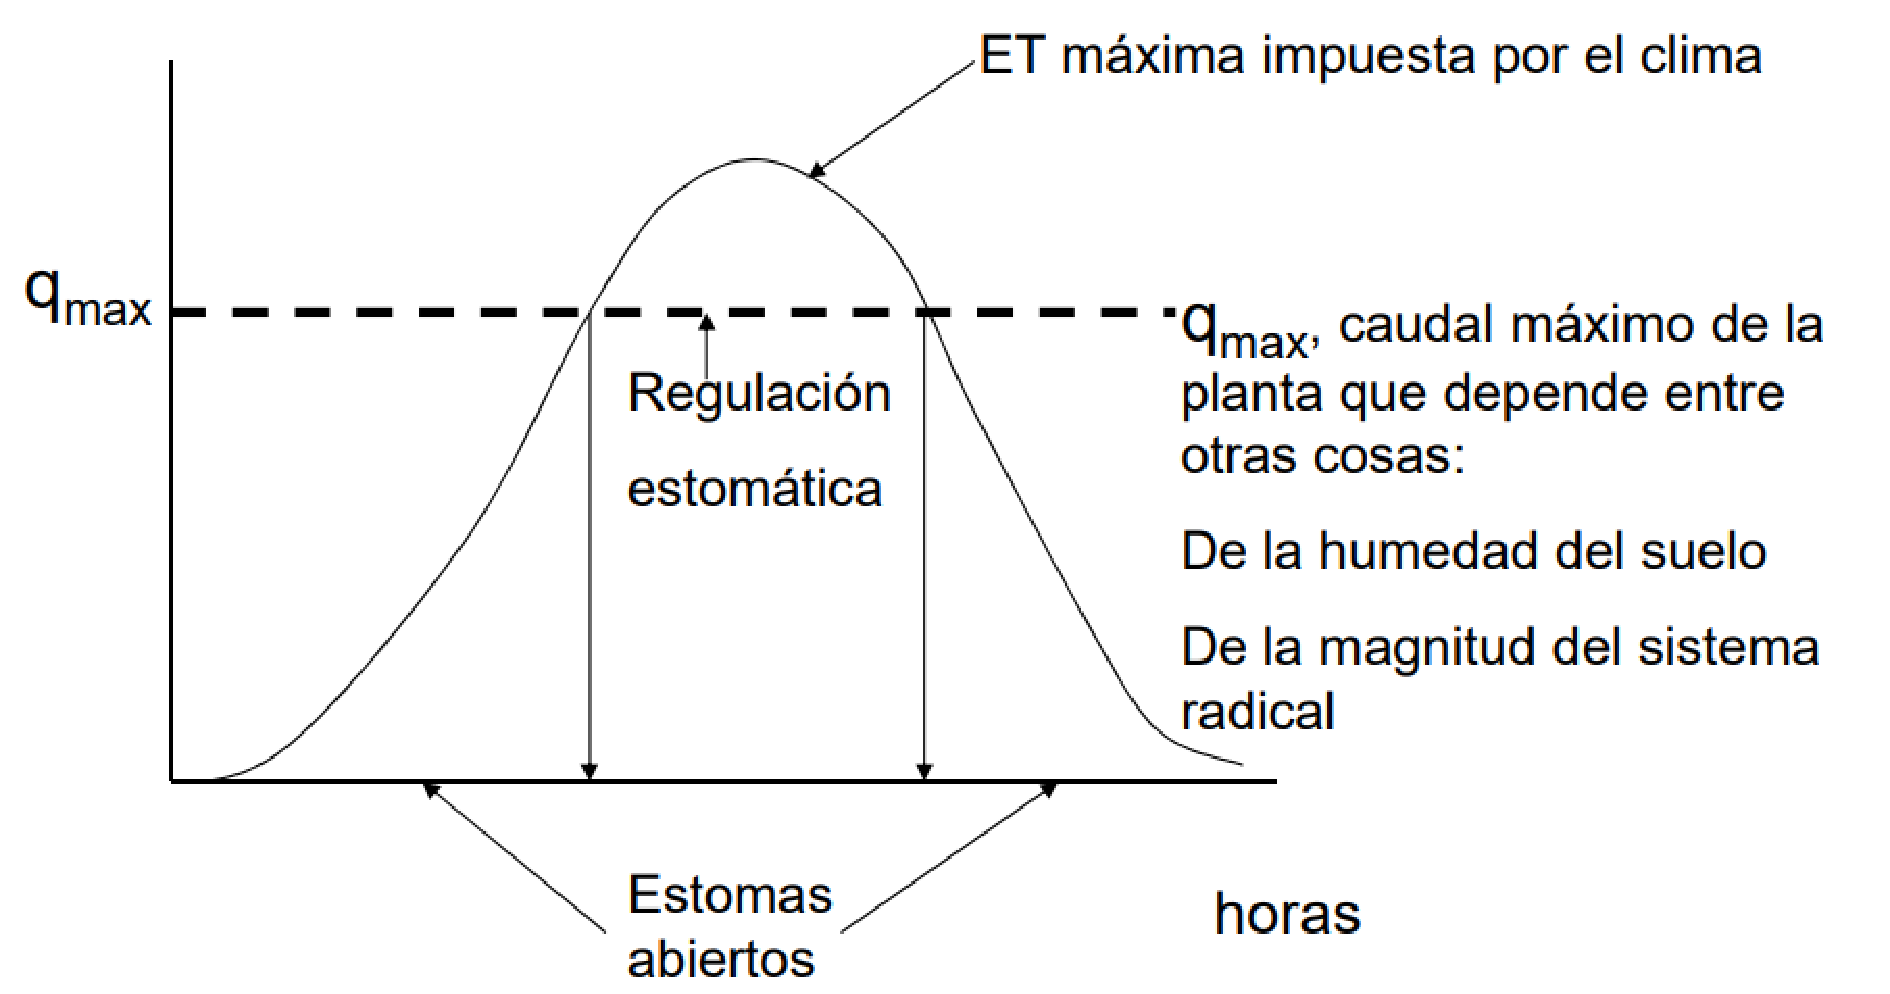
\includegraphics[width=0.5\textwidth]{ma40.pdf}
              \caption{Análisis de los elementos que intervienen en los procesos de evaporación y evapotranspiración}
              \label{ma40}
        \end{figure}
        
        \subsection{Métodos}
        
        \begin{itemize}
            \item Directos \begin{itemize}
                \item Gravimétrico
                \item Lisimétrico
                \item Evapotranspirométrico
            \end{itemize} 
            \item Indirectos \begin{itemize}
                \item Tanque tipo ``A''
                \item García y López
                \item Papadakis
                \item Linacre
                \item Jense y Haise
                \item Hargreaves
                \item Romanenko
                \item Turc
                \item Penman
                \item Método Penman-Monteith 
                \item Método Hargreaves
            \end{itemize}
            \item Atmómetros
        \end{itemize}
        
        Entrando en materia con el \textbf{método del tanque tipo ``A''}:
        \begin{equation}
            ET_o =K_p\cdot E_v
        \end{equation}
        \begin{notation}
            \begin{itemize}
                \item $ET_o$, en mm $Día^{-1}$
                \item $k_p$, coeficiente de tanque, 0.8
                \item $Ev$, evaporación de tanque tipo ``A'', en mm $Día^{-1}$
            \end{itemize}
        \end{notation}
        
        Con el método de García y López:
        \begin{equation}
            ET_o = \left[1.21 \times 10^{\frac{7.45T}{234.7 +T}} \cdot \left(1-0.01 \cdot HR \right) \right] + 0.21 \cdot T -2.3
        \end{equation}
        \begin{notation}
            \begin{itemize}
                \item $ET_o$, en mm $Día^{-1}$
                \item $T$, temperatura media , en Celsius 
                \item $HR$, humedad relativa, en porcentaje
            \end{itemize}
        \end{notation}
        Del método de Papadakis:
        \begin{equation}
            ET_o = 5.626 \cdot \left(E_{\max } -e\right)
        \end{equation}
        \begin{notation}
            \begin{itemize}
                \item $ET_o$, en mm $mes^{-1}$
                \item $E_{max}$, presión de vapor a saturación a la temperatura media máxima, en mb
                \item $e$, presión de vapor actual, en mb
            \end{itemize}
        \end{notation}
        
        Del método de Linacre:
        \begin{equation}
            ET_o = \frac{\frac{500 \cdot T_m}{100 -A} + 15 \cdot \left(T- TPR\right)}{80 -T}
        \end{equation}
        \begin{notation}
            \begin{itemize}
                \item $ET_o$, en mm $día^{-1}$
                \item $T_m=T+0.006h$
                \item $TPR$,  temperatura del punto de rocío ($^{\circ}C$)
                \item $A$, latitud del lugar
                \item $T$, temperatura media, ($^{\circ}C$)
                \item $(T-TPR)=0.0023\cdot h+0.37\cdot T+0.53\cdot R+0.35\cdot R_{año}-10.9$
                \item $R$, oscilación, ($^{\circ}C$)
                \item $R_{año}$, diferencia entre las temperaturas medias del mes más calido y el mes más frío
            \end{itemize}
        \end{notation}
        
        Para el método de Jense y Haise:
        \begin{equation}
            ET_o = \left(0.078 0.0252 \cdot  T\right) \cdot I_G
        \end{equation}
        \begin{notation}
            \begin{itemize}
                \item $ET_o$, en mm $día^{-1}$
                \item $T$, temperatura media, ($^{\circ}C$)
                \item $I_G$, radiación solar global, en mm $día^{-1}$
                \end{itemize}
        \end{notation}
        
        Con el método de Hargreaves:
        \begin{equation}
            ET_o = 0.34 \cdot I_A \cdot \left(0.4+0.024T \right)\left(1.35 \cdot \sqrt{1 -HR} \right)\left(1 +\frac{0.04 \cdot EL}{1000}\right)
        \end{equation}
        \begin{notation}
            \begin{itemize}
                \item $ET_o$, en mm $día^{-1}$
                \item $I_A$, en mm $día^{-1}$
                \item $T$, temperatura media, ($^{\circ}C$)
                \item $HR$,  humedad relativa, en decima
                \item $EL$, altura, en m
                \end{itemize}
        \end{notation}
        
        El método de Romanenko consiste en:
        
        \begin{equation}
            ET_o =0.0018 \cdot (25 +T)^2 \cdot (100-HR)
        \end{equation}
        \begin{notation}
            \begin{itemize}
                \item $ET_o$, en mm $mes^{-1}$
                \item $T$, temperatura media, ($^{\circ}C$)
                \item $HR$, humedad relativa media mensual (\%)
            \end{itemize}
        \end{notation}
        
        Del método de Turc:
        \begin{equation}
            ET_o = K \cdot \frac{T}{T +15} \cdot \left(I_G +50\right) \cdot \left(1 + \frac{50 - HR}{70}\right)
        \end{equation}
        \begin{notation}
            \begin{itemize}
                \item $ET_o$, en mm $mes^{-1}$
                \item $T$, temperatura media, ($^{\circ}C$)
                \item $I_G$, radiación global media mensual, $cal\cdot cm^{-2}\cdot Día^{-1}$
                \item $HR$, humedad relativa media mensual, en \%
                \item $K$, constante, en los meses de 30 y 31 días vale 0.4\begin{itemize}
                    \item $K$, en febrero vale 0.37
                    \item $K$, en periodos de 10 días vale 0.13
                \end{itemize}
            \end{itemize}
        \end{notation}
        
        
        Con el método de Penman:
        \begin{equation}
            ET_o =\frac{\frac{P_0}{p} \cdot \frac{\Delta}{\gamma}\left[\left(1 -\alpha\right)I_A\left(a + b\frac{n}{N}\right) -\sigma \cdot T_K^4\left(a - b \sqrt{e_d}\right) \left(a + b\frac{n}{N}\right) \right] + (E - e_d) \cdot  0.26\left(a + b \cdot U_2\right) }{\frac{P_0}{P}\cdot \frac{\Delta}{\gamma} + 1}
        \end{equation}
        \begin{notation}
            \begin{itemize}
                \item $ET_o$, en mm $mes^{-1}$
                \item $P_0$, presión atmosférica al nivel del mar, en mb
                \item $P$, presión atmosférica en función de la altitud, en mb
                \item $\Delta$, pendiente de “E” en función de la $T$, en $mb ^{\circ}C^{-1}$
                \item $\alpha$, albedo
                \item $\gamma$, constante sicrométrica
                \item $IA$ o $RA$, valor de Angot, en mm $Día^{-1}$
                \item $n$, horas brillo sol, en horas
                \item $N$, fotoperiodo, en horas
                \item $\sigma T^4_k$ expresión de Stefan-Boltzmann, en mm 
                \item $E$ o $e_a$, presión de vapor de agua a saturación, en mb
                \item $e$ o $e_d$, presión de vapor de agua actual, en mb
                \item $T$, temperatura media, en $^{\circ}C$
                \item $T_K$, temperatura en Kelvin
                \item $U_2$, velocidad del viento a 2 metros de altura, en $ms^{-1}$\end{itemize}
        \end{notation}
        Cuadro $I=IA (RA)$ implica el mes y latitud
        
        Cuadro $II=N$ implica mes y latitud
        
        Cuadro $III=\left(a+b\frac{n}{N}\right)\left(a-\alpha\right)$ implica $nN^{-1}$, así Evaporación $(1-0.05)= 0.95$ y $ET_o=(1-0.25)=0.75$
        \begin{enumerate}
            \item Regiones templadas
            \item Regiones tropicales secas
            \item Regiones tropicales húmedas
        \end{enumerate}
        
        \begin{align}
            &\text{Cuadro } IV =\sigma T^4\implies T(^{\circ}C)\\
            &\text{Cuadro } V = a - b\sqrt{e_d}\implies e_d = e(mb)\\
            &\text{Cuadro } VI = a + b\frac{n}{N}\implies nN^{-1}\\
            &\text{Cuadro } VII = e_a = E\implies T(^{\circ}C)\\
            &\text{Cuadro } VIII = 0.26\left(a + b \cdot U_2\right)\implies T_{\max} - T_{\min},U_2\\
            &\text{Cuadro } X =\frac{\Delta}{\gamma}\cdot \frac{P_0}{P}\implies \text{Altura en }m\land T(^{\circ}C)
        \end{align}
        Sí sustituimos cada uno de los cuadros en la ecuación de Penman, queda de la siguiente manera:
        \begin{equation}
            ET_o =\frac{X \cdot \left(I \cdot III - IV \cdot VI \right) + VIII\left(VII - e_d\right)}{X + 1}
        \end{equation}
Se recomienda usar las siguientes tablas para éste método:
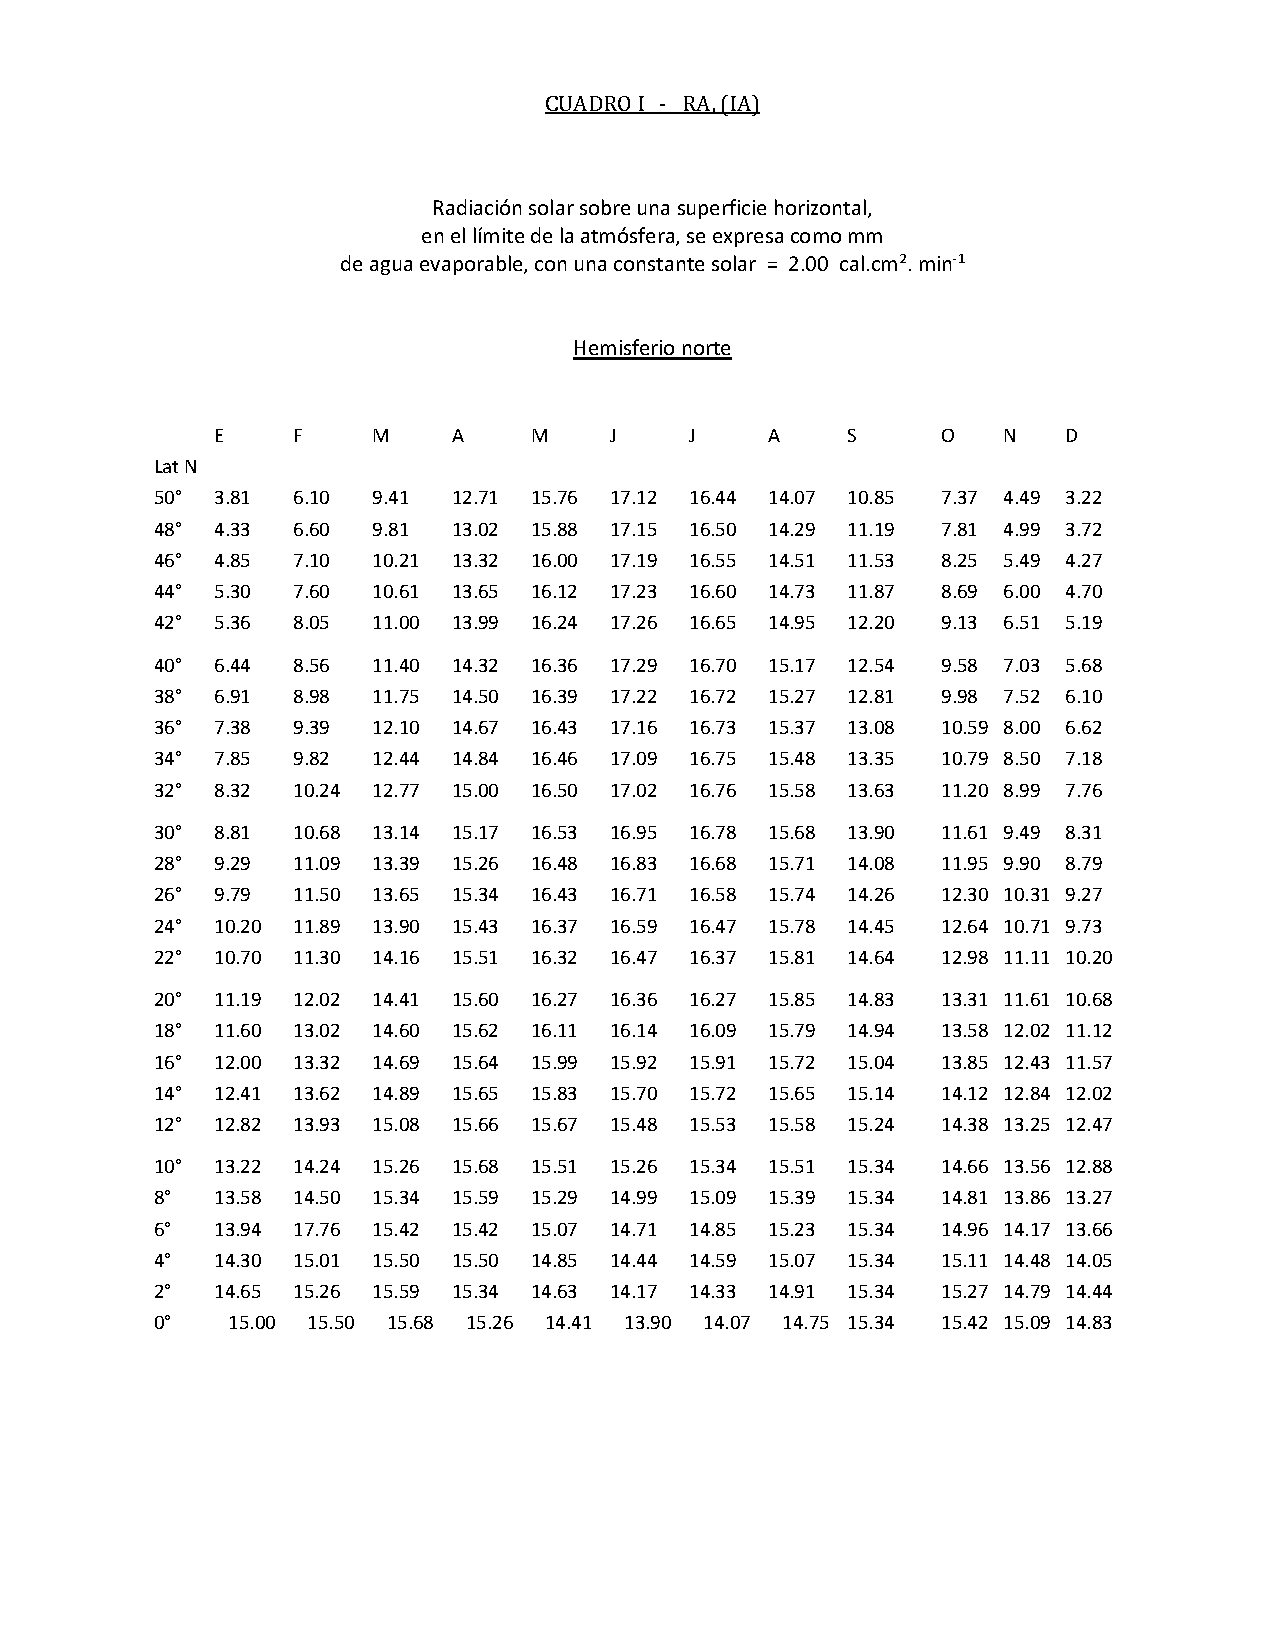
\includepdf[pages=1-15,width=1\textwidth]{ma41.pdf}
Datos para utilizar los diferentes métodos
\begin{itemize}
    \item Mes: enero
    \item Evaporación ($Ev$) = 3.95 mm $día^{-1}$
    \item Altitud = 2240 m
    \item Latitud = $19.5^{\circ}$
    \item Templado
    \item HR = 60\%
    \item Temperatura media =$ 14.4^{\circ}C$
    \item e = 10.1 mb
    \item n= 8.4 horas
    \item Temperatura media del mes más frío = $11.4^{\circ}$
    \item Temperatura media del mes más caliente = $17.3^{\circ}$
    \item Velocidad del viento a 2 m de altura = 2.4 $ms^{-1}$
    \item Temperatura máxima media = $21.4^{\circ}$
    \item Temperatura mínima media = $7.4^{\circ}$
\end{itemize}

En el método de Penman - Monteith:
\begin{equation}
    ET_0 = \frac{0.408\left(R_n - G\right) +\gamma\cdot \frac{900}{T+273}\cdot u_2\left(e_s -e_a\right)}{\Delta +\gamma\left(1 + 0.34u_2\right)}
\end{equation}
\begin{notation}
    \begin{itemize}
        \item $ET_o$, Evapotranspiración de referencia en mm $día^{-1}$
        \item $R_n=$ Radiación neta en MJ $m^2día^{-1}$
        \item $G=$ Densidad de flujo de calor del suelo en $MJ\cdot m^{-2}\cdot día^{-1}$
        \item $T=$ Temperatura media del aire a 2 m de altura en $^{\circ}C$
        \item $u_2=$ Velocidad del viento media a 2m de altura en $ms^{-1}$
        \item $e_s=$ Presión de vapor a saturación a la temperatura del aire en $kPa$
        \item $e_a=$ Presión de vapor actual en $kPa$
        \item $e_s-e_a=$ Déficit de presión de vapor en $kPa$
        \item $\Delta=$ Pendiente de la curva de presión de vapor a saturación en $kPa^{\circ}C^{-1}$
        \item Constante psicométrica en $kPa^{\circ}C^{-1}$
        \end{itemize}
\end{notation}

Finalmente el método de Hargreaves es:
\begin{equation}
    ET_o = 0.0023\left(T_{media} + 17.8\right)\cdot\left(T_{\max} - T_{\min}\right)^{0.5}(I_a)
\end{equation}
\begin{notation}
    \begin{itemize}
        \item $I_a$, Radiación solar extraterrestre, mm $día^{-1}$
        \item $T_{max}=$ Temperatura máxima diaria, $^{\circ}C$
        \item $T_{min}=$ Temperatura mínima diaria, $^{\circ}C$	
        \item $T_{media}=$ Temperatura media diaria, $^{\circ}C$
        \end{itemize}
\end{notation}
\section{Precipitación}

Su importancia radica en la Agricultura de temporal; Agricultura de riego; Recarga de acuíferos; Efectos en el terreno, del cual derivan:
\begin{itemize}
    \item Mecánica: compactación del terreno, disgregación de las partículas del suelo
    \item Acción fertilizante: de un litro de agua se aportan 2 mg de nitrógeno amoniacal y 0.7 de nitrógeno nítrico
    \item Acción química: solubilización de los minerales del suelo
\end{itemize}

\subsection{Homogeneidad de las muestras de datos climáticos}

Las series climatológicas, tales como la precipitación o temperatura son en la realidad muestras procedentes de una sola población y por ello se consideran homogéneas por definición; así como la Media, moda y mediana. Enlistando los pasos sería:

\begin{enumerate}
    \item Se requiere contar con una serie de datos de cantidad de precipitación (X) en orden cronológico
    \item Se ordenan los datos de la serie de mayor a menor y se obtiene su mediana
    \item La mediana se compara con cada uno de los valores de la serie en orden cronológico, asignando un signo mas si el valor es mayor quela mediana o negativo en caso contrario
    \item Se determina el número de cambios (NC) de positivo a negativo o el caso contrario, al NC se aumenta en la unidad y se denota como S
    \item El valor de S se compara con el intervalo (límite inferior, LI, y límite superior, LS) obtenido del cuadro 1, al cual se entra con el argumento N que es el número de años de la serie estudiada,presentándose los siguientes casos:
    \item El valor de S está comprendido dentro del intervalo: $LI\leq S\leq LS$, indica que la muestra es homogénea
    \item El valor de S es > que el LS, esto indica que la serie presenta una oscilación climática
    \item El valor de S es < que LI, esto indica que la serie tiene una tendencia climática
\end{enumerate}

\subsection{Análisis probabilístico de los datos de precipitación}

\subsubsection{De los Quintiles}
Se requiere una muestra de datos de precipitación de preferencia constituida por un número de años múltiplo de cinco, el procedimiento es:
\begin{enumerate}
    \item Serie de datos de cantidad de precipitación en orden cronológico
    \item La serie se ordena de mayor a menor
    \item La serie se divide en cinco grupos, cada grupo constará de un número de observaciones que depende de la longitud de la serie
    \item Entre cada dos grupos se determina el valor de separación por interpolación directa
    \item Cada uno de estos valores de separación, desde el más bajo al más alto se interpreta como la cantidad que será excedida respectivamente durante: 4, 3, 2 y 1 año de cada 5 años y representa por lo tanto las probabilidades del: 80, 60, 40 y 20\% respectivamente
\end{enumerate}
\subsubsection{Distribución Acumulativa de
Frecuencias}
Esta distribución proporciona la probabilidad empírica u observada, el procedimiento es:
\begin{enumerate}
    \item Serie de datos de cantidad de precipitación ($X_i$) en orden cronológico
    \item Se ordenan de mayor a menor las $X_i$
    \item A cada $X_i$ de la mayor a la menor se le asigna un número de orden $K_i$, correspondiéndole a la mayor el número 1 y así sucesivamente en forma creciente
    \item Se determina la probabilidad acumulada u observada $(F_i)$ de cada $X_i$ con la siguiente expresión: $F_i = \frac{K_i}{N+1}$, donde $N$ es el número de años de la serie
    \item Se realiza un diagrama de dispersión entre las $Fi$ contra sus $X_i$, de éste se determinan los valores o cantidades de lluvia $X_i$ para cada uno de los niveles de probabilidad de excedencia prefijados o el
    caso contrario.
\end{enumerate}

\subsection{Métodos Gráficos}

\subsubsection{Con Papel Normal}
Los primeros cuatro pasos son los mismos que los de la distribución de frecuencias acumulativas
\begin{enumerate}
    \item Se realiza una figura en papel probabilísticoNormal, entre las $F_i$ y sus $X_i$
    \item Sí se obtiene que todos los puntos de la figura realizada, presentan una tendencia lineal,entonces los datos de precipitación provienen de una distribución Normal
    \item Se traza una línea teórica a mano que mejor se ajuste a los puntos, con la cual se determinan las cantidades de precipitación $X_i$ que les corresponden a los niveles de probabilidad de excedencia prefijados o el caso contrario
\end{enumerate}
\subsubsection{Con papel LogNormal}
Se realizan los mismos pasos que en el método con papel probabilístico Normal, pero en este caso se utiliza papel probabilístico LogNorma


\subsection{Métodos Teóricos}
\subsubsection{Distribución de probabilidades Normal}
\begin{equation}
    \text{Función de Densidad }f(x)= \frac{1}{\sigma\sqrt{2\pi}}e^{-\frac{(x-\mu)^2}{2\sigma^2}}
\end{equation}
Donde $-\alpha\leq x\leq \alpha$
Estimadores de los parámetros:
\begin{align}
    &\text{Media }\mu=\bar{x}=\frac{1}{N}\sum_{i=1}^{N}x_i\\
    &\text{Varianza }\sigma^2=\frac{1}{N-1}\sum_{i=1}(x_i-\bar{x})^2\\
    &\text{Desviación estándar }\sigma= S_x=\sqrt{S_x^2}
\end{align}

Serie de datos de cantidad de precipitación ($X_i$) en orden cronológico

Se ordenan las $X_i$ de mayor a menor

Se calcula la media y la desviación estándar de las $X_i$

Se determina el valor estandarizado $(Z_i)$ de cada $X_i$

Se calcula la probabilidad de excedencia $P(Z\geq z)$y se realiza una figura entre las $X_i$ con su probabilidad de excedencia, de ésta se puede definir la cantidad de precipitación ($X_i$) que le corresponde a un nivel de probabilidad prefijado o la condición contraria.

\subsubsection{Distribución de probabilidades LogNorma}
En este caso se transforman las variables originales ($X_i$) obteniendo sus logaritmos naturales que se denota como Yi ($Y_i=\ln{\left(X_i\right)}$), y se sigue el mismo procedimiento que la distribución Normal, la probabilidad de excedencia que se calcula se le asigna al valor original $X_i$
\subsubsection{Distribución de probabilidades Raíz Cúbica}
En este caso se transforman las variables originales $(Xi)$ obteniendo sus raíces cúbicas que se denota como $W_i\mid (Wi=X_i^{1/3})$, y se sigue el mismo procedimiento que la distribución Normal, la probabilidad de excedencia que se calcula se le asigna al valor original $X_i$

\subsubsection{Aplicación del análisis probabilístico de la precipitación}
Determinación del inicio de la época de siembra con cantidad de precipitación
\begin{figure}[h!]
    \centering
      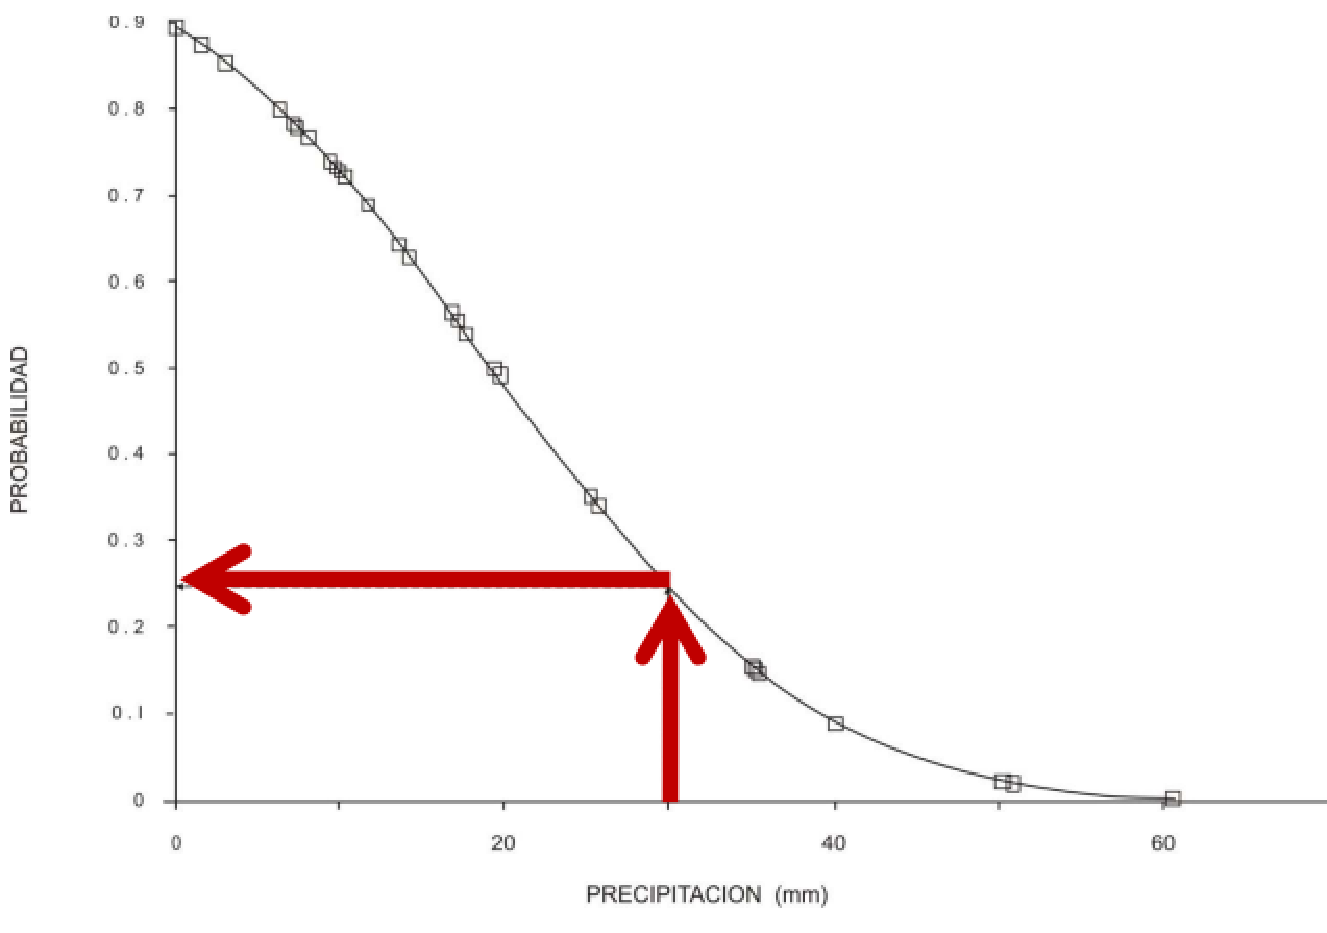
\includegraphics[width=0.5\textwidth]{ma42.pdf}
      \caption{Análisis probabilístico de precipitación de una decena}
      \label{ma42}
    \end{figure} 
    \subsubsection{Análisis probabilístico de datos de lluvia con eventos de no lluvia}
\begin{enumerate}
    \item Serie de datos de lluvia en orden cronológico 
    \item Se contabilizan los eventos con lluvia $X_i$ y el total de datos se denota como $(M)$ y se dividen entre el total de datos de la serie (N) 
    \item Se determina la constante C = M/N 
    \item El análisis probabilístico se realiza únicamente con la serie que tiene datos de lluvia o para valores prefijados de lluvia. 
    \item A la serie de datos de lluvia se le determina su media y su desviación estándar 
    \item Se determinan los valores de $Z$ para los valores de la serie de precipitación o para valores prefijados 
    \item Se determina la probabilidad de X > x, y a esta probabilidad se le multiplica por la constante y el resultado es la probabilidad que se está buscando.
\end{enumerate}

    \section{Balance hídrico}
    Como aplicaciones se pueden enlistar las siguientes:
    \begin{enumerate}
        \item Planeación de los recursos hidráulicos
        \item Clasificaciones climáticas y agroclimáticas
        \item Manejo de suelos
        \item Pronóstico de inundaciones y sequías
        \item Fluctuaciones de nivel del mar
        \item Pronósticos de incendios forestales
        \item Zonificación de cultivos en áreas de temporal
        \item Determinación de los periodos de deficiencias o excesos\\
     Pronóstico del momento de riego
        \item Estimación del consumo de agua de los cultivos
        \item Elaboración de calendarios agrícolas
        \item Predicción del rendimiento
    \end{enumerate}
    \begin{figure}[h!]
    \centering
      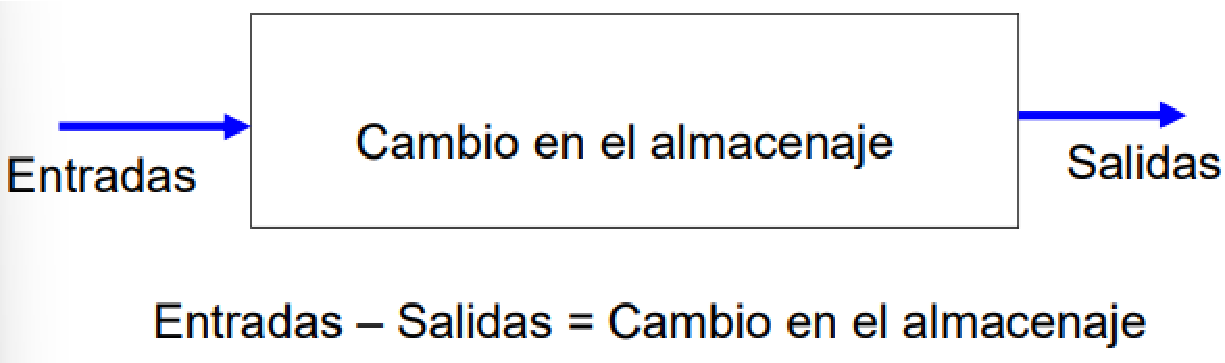
\includegraphics[width=0.5\textwidth]{ma43.pdf}
      \caption{Ley de conservación de la materia}
      \label{ma43}
    \end{figure}
    \begin{definition}[Balance hídrico]
        Thornthwaite y Mather (1966) consideran que la humedad del suelo es un equilibrio entre la precipitación que penetra al mismo y la que sale en forma de evaporación de agua del suelo y la transpiración de la vegetación
    
    Grassi (1968) Al confrontar los valores de evapotranspiración de referencia en un determinado periodo, con la precipitación que ocurrió durante éste se conocen las deficiencias o los excesos de agua. Además dado que el suelo tiene la capacidad de almacenar agua, ésta debe tomarse en cuenta.
    
    Norero (1976) Conceptualiza este método como la formulación matemática de la ley de conservación de la materia, en este caso el agua en el suelo y según lo cual, la cantidad de agua almacenada en un volumen determinado debe igualar a la diferencia entre los ingresos y egreso de agua
    
    Baldión (1988) lo define como la utilización de los datos reales de precipitación y de información climatológica para el cálculo de las necesidades de agua de los cultivos
    \end{definition}
    Los componentes del Balance hídrico y la ecuación general:
    \begin{equation}
        S_i = S_{i - 1}+P_i+I_i+C_i+FSSE_i-ET_i-R_i-DP_i-FSSS_i
    \end{equation}
    
    \begin{notation}
    \begin{itemize}
        \item $P$, precipitación
        \item $I$, riego
        \item $C$, ascenso capilar
        \item $FSSE$, flujo subsuperficial
        \item $ET$, evapotranspiraciónR, escurrimiento
        \item $DP$, percolación
        \item $FSSS$, flujo subsuperficial
        \item $S$, almacenamiento del suelo
    \end{itemize}
    \end{notation}
    
    La ecuación del balance hídrico climático es:
    \begin{equation}
        HA_i=HA_{i- 1}+P_i-ETO_i
        \begin{cases} 
            &\text{Sí }HA_{i-1}+P_i-ETO_i<0\implies\text{ Deficiencia}\\  
            &\text{Sí }HA_{i-1}+P_i-ETO_i >CA\implies\text{ Exceso}\\
            &\text{Sí }HA_{i- 1}+P_i-ETO_i\leq CA\implies HA
        \end{cases} 
    \end{equation}
    
    \subsection{Balance hídrico climático tipo Thornthwaite}
    \begin{notation}
        \begin{itemize}
            \item $CA$, capacidad de almacenamiento
    
            \item $Ev$, evaporación del tanque tipo ``A'' 
            \item $ETO$, evapotranspiración de referencia, $ET0 = 0.8\cdot Ev $
            \item $P$, Precipitación
            \item $P- ET0$, deficiencia o exceso climático
        \end{itemize}
        \end{notation}
    
    \begin{align}
        &\text{Humedad almacenada }HA \implies HA_i=HA_{i-1}+P_i-ETO_i\\
        &\text{Variación de almacenaje }VA \implies VAi =HA_i -HA_i- 1\\
        &\text{Evapotranspiración real }ETR_i \implies\text{ Sí }P_i > ETO_i \implies ETR_i = ETO_i\\
        &Sí P_i < ETO_i \implies ETR_i = P_i +\left\lvert VA_i \right\rvert \\
        &\text{Deficiencias }Def \implies Def_i = ETO_i - ETR_i \\
        &\text{Excesos }EXC \implies HA_{i- 1}+ P_i-ETO_i > CA\\
        &\text{Escurrimiento }ESC \implies ESC_i = \frac{EXC_{i-1}}{4} + \frac{EXC_i}{2}
    \end{align}
    \begin{figure}[h!]
    \centering
      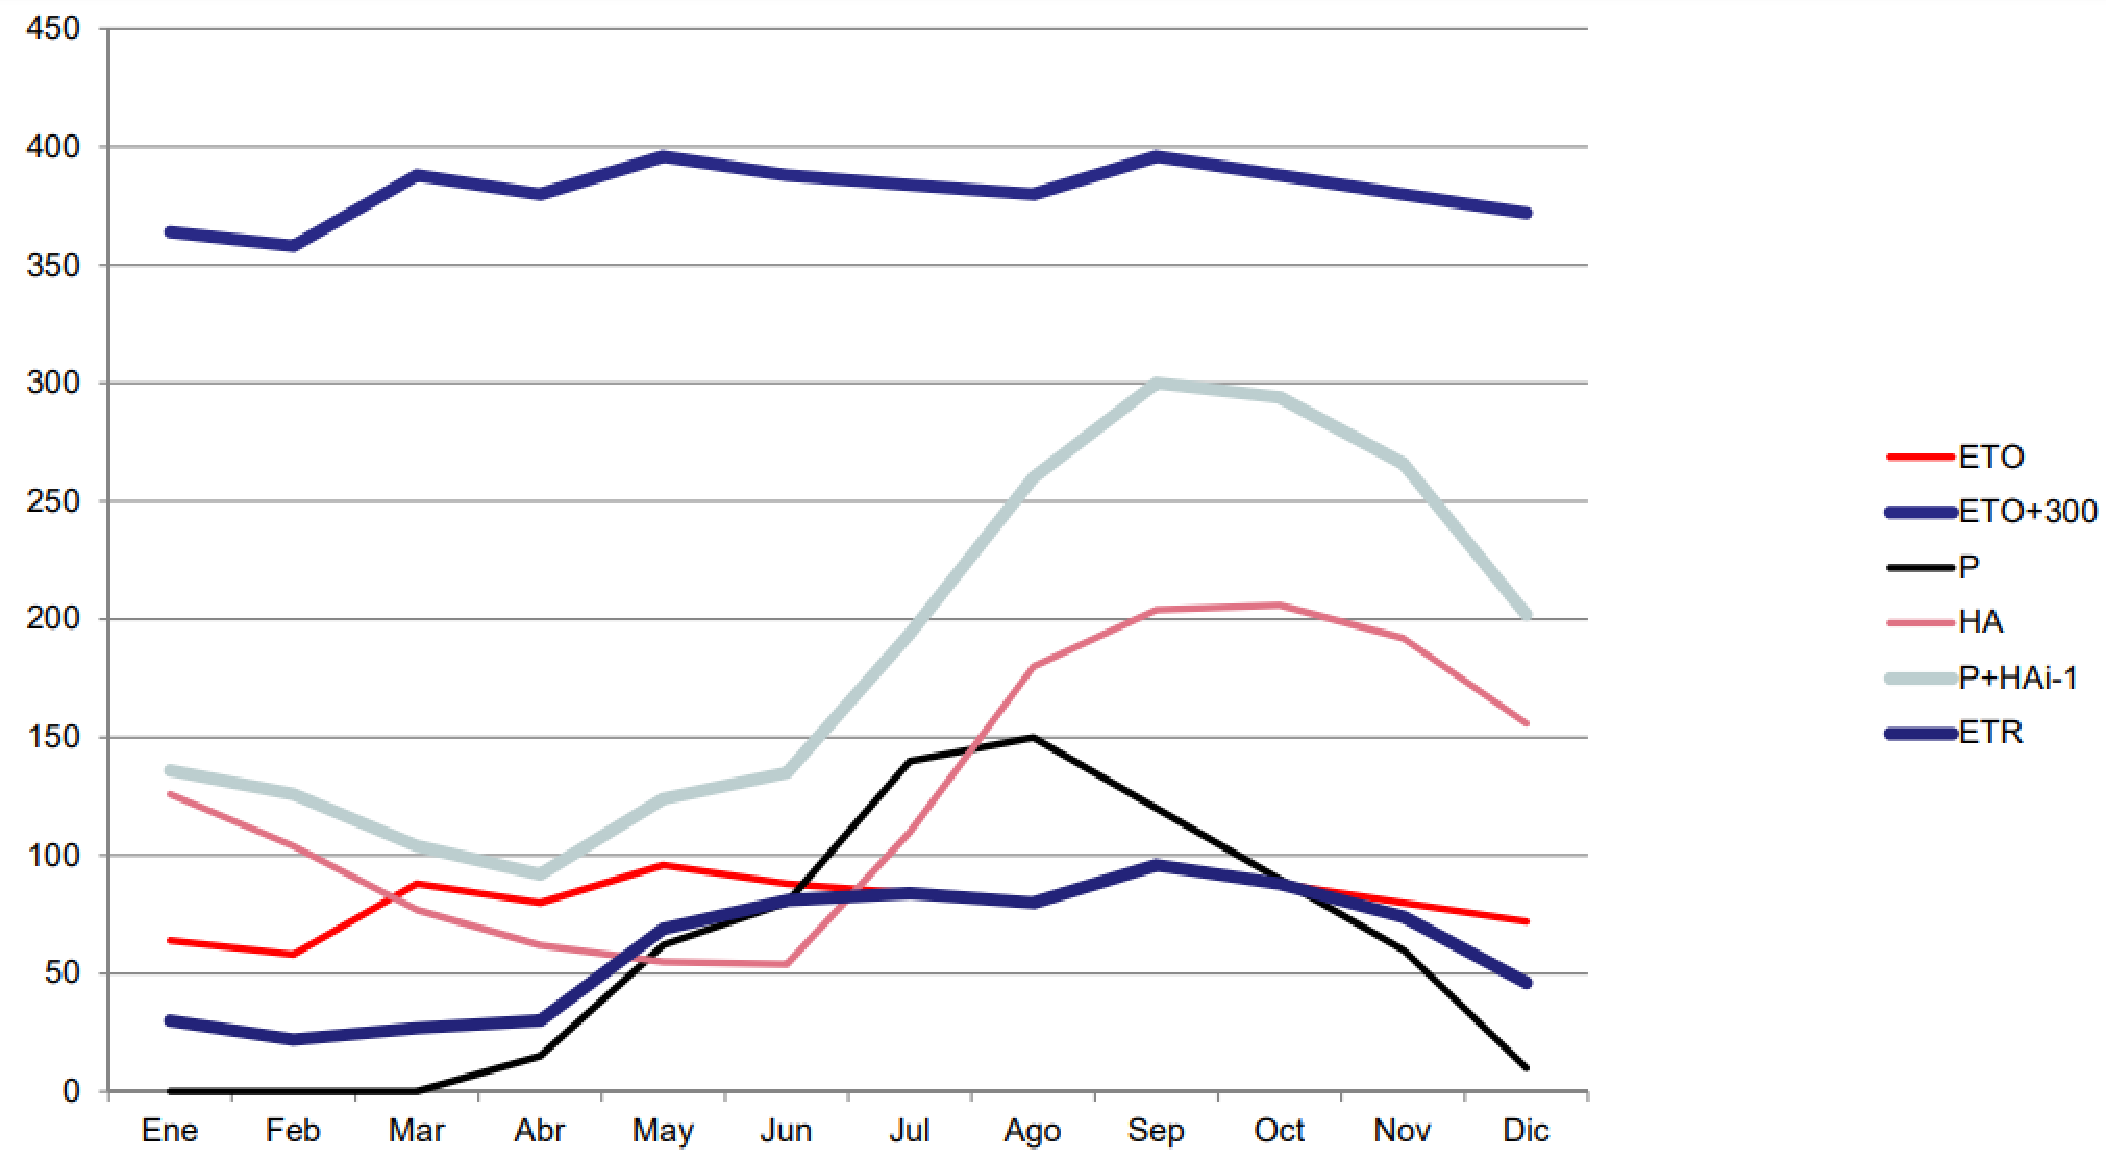
\includegraphics[width=0.5\textwidth]{ma44.pdf}
      \caption{Climodiagrama}
      \label{ma44}
    \end{figure}


































